% !TEX TS-program = pdflatex
% !TEX encoding = UTF-8 Unicode

% This is a simple template for a LaTeX document using the "article" class.
% See "book", "report", "letter" for other types of document.

\documentclass[11pt]{article} % use larger type; default would be 10pt

\usepackage[utf8]{inputenc} % set input encoding (not needed with XeLaTeX)

%%% Examples of Article customizations
% These packages are optional, depending whether you want the features they provide.
% See the LaTeX Companion or other references for full information.

%%% PAGE DIMENSIONS
\usepackage{geometry} % to change the page dimensions
\geometry{a4paper} % or letterpaper (US) or a5paper or....
% \geometry{margin=2in} % for example, change the margins to 2 inches all round
% \geometry{landscape} % set up the page for landscape
%   read geometry.pdf for detailed page layout information

\usepackage{graphicx} % support the \includegraphics command and options

% \usepackage[parfill]{parskip} % Activate to begin paragraphs with an empty line rather than an indent

%%% PACKAGES
\usepackage{booktabs} % for much better looking tables
\usepackage{array} % for better arrays (eg matrices) in maths
\usepackage{paralist} % very flexible & customisable lists (eg. enumerate/itemize, etc.)
\usepackage{verbatim} % adds environment for commenting out blocks of text & for better verbatim
\usepackage{subfig} % make it possible to include more than one captioned figure/table in a single float
% These packages are all incorporated in the memoir class to one degree or another...

\usepackage{latexsym}
\usepackage{graphicx}
\usepackage{mathptmx}

\usepackage{eurosym}
\usepackage{subfig}
\usepackage{color}

%
%****************************************************************************
% AUTHOR: You may want to use some of these packages. (Optional)
\usepackage{amsmath}
\usepackage{amsfonts}
\usepackage{amssymb}
\usepackage{amsbsy}
\usepackage{amsthm}


%%% HEADERS & FOOTERS
\usepackage{fancyhdr} % This should be set AFTER setting up the page geometry
\pagestyle{fancy} % options: empty , plain , fancy
\renewcommand{\headrulewidth}{0pt} % customise the layout...
\lhead{}\chead{}\rhead{}
\lfoot{}\cfoot{\thepage}\rfoot{}

%%% SECTION TITLE APPEARANCE
\usepackage{sectsty}
\allsectionsfont{\sffamily\mdseries\upshape} % (See the fntguide.pdf for font help)
% (This matches ConTeXt defaults)

%%% ToC (table of contents) APPEARANCE
\usepackage[nottoc,notlof,notlot,other]{tocbibind} % Put the bibliography in the ToC
\usepackage[titles,subfigure]{tocloft} % Alter the style of the Table of Contents
\renewcommand{\cftsecfont}{\rmfamily\mdseries\upshape}
\renewcommand{\cftsecpagefont}{\rmfamily\mdseries\upshape} % No bold!

%%% END Article customizations

%%% The "real" document content comes below...

\title{ABMS OPTIMIZATION FOR EMERGENCY DEPARTMENT}
\author{Eduardo Cabrera\\
Emilio Luque\\ [12pt]
CAOS, Edifici Q1\\
Universitat Aut\`onoma de Barcelona (UAB)\\
E-08193, Bellaterra, SPAIN
\and
Manel Taboada \\\\[12pt]
Tom\`as Cerd\`a Computer Science School\\
Universitat Aut\`onoma de Barcelona (UAB)\\
E-08174 Sant Cugat, SPAIN
\and
Francisco Epelde \\
        Ma Luisa Iglesias \\[12pt]
        Hospital of Sabadell\\
Corporaci\'o Sanit\`aria Parc Taul\'i \\
Parc Taul\'i, 1 \\
E-08208 Sabadell, SPAIr}
%\date{} % Activate to display a given date or no date (if empty),
         % otherwise the current date is printed 

\begin{document}
\maketitle

\section*{Abstract}
An agent-based modeling and simulation to design a decision 
support system for healthcare emergency department (ED) to aid in setting up 
management guidelines to improve it is presented. This research is being performed 
by the Research Group in Individual Oriented Modeling at the Universitat
Aut\`onoma de Barcelona with close collaboration of the hospital staff team of Sabadell. The 
objective of the proposed  procedure is to optimize the performance of such 
complex and dynamic healthcare EDs, which are overcrowded. Exhaustive search optimization is used to 
find the optimal ED staff configuration, which includes doctors, triage nurses, and admission personnel, the amount, and sort of them, i.e., a multi-dimensional and multi-objective problem. Three different indexes were set. The model is implemented using NetLogo. The results obtained by using alternatives Monte Carlo and Pipeline schemes are promising. The impact of these schemes to reduce the computational resources used  is described.

Nowadays, many of the healthcare systems are large, complex environments and quite dynamic, specifically Emergency Departments, EDs. They are opened and working 24 hours per day throughout the year with limited resources. EDs are usually the main entrance to the hospital, and a key component of the whole healthcare system. The original mission of EDs is to primarily handle only emergency situations. However, ED visits include a wide range of illnesses and injuries, from truly emergencies to non-urgent cases. As a consequence, EDs are overcrowded. Thus, is mandatory to use extensively computer simulations of EDs to evaluate output responses. The choice of optimal simulation parameters can lead to improved functioning, but choosing a good configuration remains a challenging problem. This improvement can be achieved by modelling and simulating EDs using Agent-Based Modelling and simulation. Optimisation via simulation is an emerging field which integrates optimisation techniques into simulation analysis. 

In this research a two-phase optimisation methodology for optimisation via simulation for healthcare Emergency Departments is proposed. The first phase is a coarse grained approach consisted in a global exploration step over the entire search space. This phase identifies promising regions for optimisation based on a neighbourhood structure of the problem, using either a pipeline scheme approach of an Emergency Department or the Monte Carlo heuristic plus the K-means method, or both. This first phase returns a collection of promising regions. The second phase is a fine grained approach that consists in seeking the best solution, either the optimum or a sub-optimum by performing a “reduced exhaustive search” in such promising regions. 


%------------------------------------------------------------------------- 
\section{Introduction}
\label{sec:intro}

Health is one of the most appraised gifts for human beings; therefore, it is crucial to preserve it. Healthcare units were designed to 
take charge of it. Healthcare systems have evolved during the previous decades, specifically emergency departments (ED). ED is a 
primary healthcare department, usually the main entrance to the hospital, and a key component of the whole healthcare system. EDs 
are semi-autonomous units that are open and staffed 24 hours per day, 365 days per year, including holidays. The original mission of 
EDs is to primarily handle only emergent situations. However, ED visits include a wide range of illnesses and injuries, i.e., truly 
emergencies, urgent, semi-urgent, and non-urgent cases. EDs have increased their resources to attend all of those cases, becoming large, complex and dynamic units. In spite of such an increase, patients continue to suffer, since they do not have access to ad hoc
healthcare, in some cases due to the inefficiencies of the EDs functioning. As a result of this,  EDs are overcrowded and the length of 
stay (LoS) of patients has increased, whereas quality of service has decreased. Indeed, overcrowding of EDs is a worldwide issue, 
and a national crisis in the US \cite{national2007}. Although ED overcrowding is not a new topic, since it was documented in the 
literature 20 years ago \cite{Lynn1991287}, there is not a solution to this long and growing issue yet. Despite that EDs are under this 
overcrowding phenomena, they have suffered budget reductions. Therefore, new techniques and paradigms should be found  in 
order to deal with such overcrowded condition. ED managers require different and fresh solutions, because society demands not only 
care, quality and service, but also the best care, quality and service. A direct solution to this issue is increasing the size of EDs. 
However, this straightforward solution is limited by the facility, number of staff (doctors, nurses, technicians) and services 
(computing, communication, radiology, laboratory), and it is not the best approach.  Also, healthcare managers have to maximize the 
use of healthcare resources, whereas being constrained by limited budget, in order to minimize patient LoS, while increase 
satisfaction of the patients, i.e., to optimize the performance of the ED. The resource planning of an ED is complex activity, since it is 
not linear, and it varies depending on time, day of week and season. The ability to simulate special situations such as seasonal 
increases in ED demand can be useful for the efficient use of resources. There are no standard models to describe a complex system. 
Simulation becomes an important tool for modeling systems including many elements as well as interdependencies among the 
elements, and/or considerable variability. Discrete event simulation (DES), system dynamics (SD) and agent-based modeling and 
simulation (ABMS) are the three main approaches used to simulate healthcare systems. There are a large and  growing body of 
literature describing the use of DES and SD models in ED studies, but the use of ABMS for this purpose is few; although healthcare 
systems are based on human actions and interactions that are quite difficult to model with DES, and can be more properly modeled 
with ABMS. 

This article presents the results of a research project that is being carried out by the Research Group in Individual Oriented 
Modeling (IoM) in the Universitat Aut\`onoma de Barcelona (UAB), with the participation of the ED managers of the Hospital of 
Sabadell  (one of the most important Hospitals in Spain that gives care service to an influence area of 500,000 people, and attends 
160,000 patients/year in the ED). The general objective of the project is to develop an ED simulator that, used as a decision support 
system (DSS), aids the managers of EDs in setting up strategies, and management guidelines to enhance the efficiency of such EDs. 
The specific objective is to implement in the proposed DSS model an algorithm to optimize the number of staff members of EDs, 
including admission staff, triage nurses, and doctors, under certain economical and operational constrains. 

This work optimises the sanitary staff configuration of an actual ED. The sanitary staff configuration comprises: doctors, triage and emergency nurses, admission personnel, and x-ray technicians, the amount, and sort of them. Staff configuration is a combinatorial and multidimensional problem, that can take a lot of time to be solved. In order to do optimisation, objective functions to minimise or maximise have to be set. Three different indexes were set: minimise patient length of stay (LoS); maximise number of attended patients per day (Throughput); and minimise a compound index, the product of the cost of a given sanitary staff configuration times patient length of stay (CLoS). HPC is used to run the experiments, and encouraging results were obtained. However, even with the simplified ED used in this work the search space is very large, thus, when the problem size increases, it is going to need more resources of processing in order to obtain results in a reasonable time.

A good monitoring system will alert you to issues before they become problems and allow you to focus 
on your core business and not reacting to IT issues. 

The Emergency Department model defined herewith is a pure Agent-Based Model (ABM), and so is formed entirely of the rules 
governing the behavior of the individual agents that populate the system. The system behavior emerges as a result of local level 
actions and interactions. This model describes the complex dynamics found in an ED, representing each individual and system as 
an individual agent. 

The rest of this article is organized as follows; Section ~\ref{sec:review} describes the literature review. The ED model is succinctly 
described in Section ~\ref{sec:ed-mdl}, the mathematical-computational model of the ED are presented in Section ~\ref{sec:math-comp}, the optimization problem of interest, the experiment, and the results of three simulation optimization techniques are given in 
Section ~\ref{sec:optimal}, the proposed methodology to find the optimum is described in Section ~\ref{sec:mc_pipe}. Finally,  the 
conclusions and future work  are presented in Section ~\ref{sec:conclu}.

%------------------------------------------------------------------------- 
\section{Related Work}
\label{sec:review}

In 1979 computer simulation was applied to hospital systems to improve the scheduling of staff members \cite{Hancock:1979p28}, 
and in \cite{Saunders:1989p134} the aim was to quantify the impact that the amount of staff members and beds had on patient 
throughput time. Moreover, a survey  of discrete-event simulation in healthcare clinics was presented in 1999 
\cite{Jacobson:1999p109}.

Although, discrete-event simulation is widely used in simulating healthcare systems, agent technology is most suited to be used in 
healthcare applications, because it characterizes better the operation of complex systems such as EDs. 
There is a relevant article which uses ABM to simulate the work flow in ED \cite{Lu:2009p19}. It focus on triage and radiology processes, but not real data is used, the acuity of patients are not considered, and healthcare providers do not always serve patients in a first-come-first-serve basis.
Simulation optimization is used to improve the operation of ED in \cite{Ruohonen:2006p453}, using a commercial simulation package, and \cite{Ahmed:2009p936} combines simulation with optimization, which involves a complex stochastic objective function under deterministic and stochastic sets of restrictions. Also, in \cite{Weng:2011p1231} system simulation is used to improve the flow of the ED using an index to measure the degree of congestion of ED.
Previous works on modeling healthcare systems have focused on patient scheduling under variable pathways and stochastic process 
durations, the selection of an optimal mix for patient admission in order to optimize resource usage and patient throughput 
\cite{Hutzschenreuter:2008p42}. Work has been performed evaluating patient LoS under the effects of different ED physician 
staffing schedules, and the only one found until now that utilizes real data is \cite{Jones:2008p338} or patient diversion strategies 
\cite{Laskowski:2008p25}.
An evolutionary multi-objective optimization approach is using for dynamic allocation of resources in hospital practice 
\cite{Hutzschenreuter:2009p320}, while in \cite{Persson:2005p260} it was found that  combining agent-based approaches and 
classical optimization techniques complement each other. 

This proposal addresses many of the issues surrounding the modeling and simulation of a healthcare emergency department using 
agent-based paradigm, where the efficiency of agents in this area has not been totally explored yet. The basic rules governing the 
actions of the individual agents are defined in an attempt to understand micro level behavior. The macro level behavior, that of the 
system as a whole, emerges as a result of the actions of these basic building blocks, from which an understanding of the reasons for 
system level behavior can be derived \cite{Stainsby:2009p536}. \\

%------------------------------------------------------------------------- 
\section{Problem Modeling}
\label{sec:pm}

%------------------------------------------------------------------------- 
\subsection{Agent-Based Model of Emergency Department}
\label{ssec:ed-mdl}

In this Section, a brief description of the proposed Agent-Based Model (ABM) is presented. The Emergency Department model defined by this work is a pure ABM, thus it is formed entirely of the rules governing the behavior of the individual agents which populate the system, no higher level behavior is modeled. The system behavior emerges as a result of local level actions and interactions. This model describes the complex dynamics found in an ED, representing each individual and system as an individual agent. 
Two distinct kinds of agents have been identified, active and passive. Active agents represent the individuals involved in the ED, in this case all human actors, such as patients and ED staff (admission staff, nurses, doctors, etc). Passive agents represent services and other reactive systems, such as the information technology (IT) infrastructure or services used for performing tests. Moore State machines are used to represent the actions of each agent. This takes into consideration all the variables that are required to represent the many different states that such individual (a patient, a member of hospital staff, or any other role) may be in throughout the course of their time in a hospital emergency department. The change in these variables, invoked by an input from an external source, is modeled as a transition between states. In some specific cases the state machine involves probabilistic transitions, where a given combination of current state and input has more than one possible next state. Which transition is made is chosen at random at the time of the transition, weights on each transition provide a means for specifying transitions that are more or less likely for a given individual. Probabilities may be different for each agent. In this way heterogeneity is provided to agents as people, since agent behavior can be probabilistically defined external to their state. The communication between individuals is modeled as the inputs that agents receive and the outputs they produce, both implicitly and explicitly. The communication model represents three basic types of communication. The first type is 1-to-1 communication, such as between two individuals, for instance admission staff and patient, where a message has a single source and a single destination, as well as between patients, or staff personnel. The second type is 1-to-n communication, where a message has a single source and a specific set of recipients, for example when a doctor communicates with both patient and his companion, or when doctor communicates with other doctors and nurses. The last type is 1-to-location communication, where a message has a single source, but it is received by every agent within a certain area or location. This occurs when a triage nurse sends a message to the patients in the waiting room, through the loudspeaker system. In order to control the agent interaction, the physical environment in which these agents interact also has to be modeled, such as admissions, triage box, the waiting room, and consultation suits. A detailed description of the emergency department model using the agent-based paradigm can be found in the following article \cite{Manel:2011p1870}


%------------------------------------------------------------------------- 
\subsection{Mathematical-Computational Model of Emergency Department}
\label{ssec:math-comp}

\subsubsection{Multi-Objective Optimization}
\label{sssec:mop}

From the mathematical point of view, the optimization problem stated in Section ~\ref{sec:intro} is to optimize the number of staff members of an ED under specific economical and operational constraints. This problem can be formulated as a multi-objective optimization problem which is formally defined as follows: 
Find the vector $ \vec{x}^* = [ x^*_1 , x^*_2 ,..., x^*_n ]^T $ which optimizes the vector function:

\vspace{-0.05cm}
\begin{equation*}  \label{eq:Opt}
\vspace{-0.05cm}
\begin{aligned}
& {\text{max / min}}
& & \vec{f}(\vec{x}) = [ f_1(\vec{x}), f_2(\vec{x}), ..., f_k(\vec{x})]^T \\
& \text{subject to}
& & g_i(\vec{x}) \leq 0 \quad  i = 1,2,...,m \\
& &  & h_i(\vec{x}) = 0 \quad i = 1,2,...,p
\end{aligned}
\tag{1}
\end{equation*}

\noindent where $f_i$ is the $i-th$ objective function.  $x^*_i$ is a discrete vector, global sampling of $\vec{x}^*_i$ is possible to get, but not all of $f_i(x^*_i)$ can be evaluated exactly, and must be estimated via a simulation procedure. Since  several objective functions exist, instead of looking for a single solution, an acceptable or trade-off solutions it is trying to find them. It is say that a vector of decision variables $ \vec{x}^* \in PO$ is {\it Pareto optimal} if $ \nexists $ another $ \vec{x} \in PO $ such that $ f_i(\vec{x}) \leq f_i(\vec{x}^*) \quad  \forall i=1,...,k ) $ and $ f_j(\vec{x}) < f_j(\vec{x}^*)$ for at least one $j$. $PO$ represents the feasible region of the problem,  i.e., where the constraints are satisfied. The goal of the optimization procedure is to identify the staff members of the EDs that optimize their performance, which needs to be estimated via a simulation due to the complexity of EDs. Optimization via simulation is a difficult task \cite{Fu:2002p192}. As simulations are usually computationally expensive, even estimating $f_i(x^*_i) $ at a single point in Equation \eqref{eq:Opt} may require substantial effort, which implies that only some scenarios would be explored. Three different alternatives used in this work are briefly described following. 

\subsubsection{Exhaustive Search}
\label{sssec:exh}

Exhaustive search (ES) is used for discrete and combinatorial problems in which no efficient solution technique is known. In order to determine the solution it might be necessary to test each possibility and verify if it satisfies the statement of the problem. If there exists a solution, then ES technique will always find such solution. Nevertheless, the computational cost is high and proportional to the number of possible solutions which could be quite large, i.e., a combinatorial explosion. 

\subsubsection{Monte Carlo}
\label{sssec:mc}

Monte Carlo (MC) is a statistical sampling method used to approximate solutions to quantitative problems. It is widely used when it is infeasible to compute an exact solution using a deterministic algorithm, there are many degrees of freedom, or incertitude in the input data. MC method does not suffer from the curse of dimensionality. In order to reduce the standard error, different techniques  could be used, among them are increasing the sample size and variance reduction.

\subsubsection{Pipeline}
\label{ssec:pipe}

This technique is usually known as assembly line. It consists of several ordered stages. The output of one stage is the input of the next one. Once the second stage is working, the first stage is attending the next input, and so on. Therefore, when the hole pipeline is full, one output per time is obtained. All stages could be configured to have more than one unit, i.e., parallel stages. So, not only the throughput but also the pipeline of the system is enhanced. However, when the process between each stage cannot be synchronized the use of buffers ought to be necessary. The pipeline time can be expressed by Equation  \eqref{eq:Pipe}, where $ S_i $ represents each stage of the pipeline.

\vspace{-0.05cm}
\begin{equation*}  \label{eq:Pipe}
\vspace{-0.05cm}
\begin{aligned}
& {\text{Pipeline time }} \:  = \cfrac{1}{ \sum \cfrac{1}{S_1} } + \cfrac{1}{ \sum \cfrac{1}{S_2} } + ... + \cfrac{1}{ \sum \cfrac{1}{S_k} }  \\
\end{aligned}
\tag{2}
\end{equation*}

%------------------------------------------------------------------------- 
\section{Optimization}
\label{sec:optimal}

\subsection{The Problem}
\label{sec:desc}

The optimization problem  considered in this paper and expressed by Equation \eqref{eq:Opt} aims to find the best ED staff configuration: doctors (D), triage nurses (N), and admissions (A), which optimize the ED's functioning. The simplified  patient flow in the ED is defined as follows:  Patients arrive to the ED on their own, and waits to be attended in the admission area. Then, patients stay in the first Waiting Room (WR), WR1, until a triage nurse calls them. After the triage process, patients pass to a second WR2, and stay there until a free doctor calls them to begin the diagnosis and treatment phase, depending on the patient's symptoms and physical condition, as well as prescribed tests. At the end, patients are discharged from the ED. Even though realistic treatment is based on the acuity of patients they have the same path throughout the ED at this moment in this research project.

%The present scenario adopted for the experiments is to simulate patients moving through a simplified ED that includes four primary %areas: admissions, 3 triage boxes, 2 waiting rooms, and the 4 diagnosis and treatment boxes. In order to validate the simulator, %basic patient attributes were set as well as a simple patient flow defined previously.

For simplicity, only four different types of active agents are considered: patients, admission staff, nurses, and doctors. Staff  considered characteristics are shown in Figure \ref{fig:combs} and Table \ref{tab:T1}. Taking into account: a) that each of the personnel staff has two levels of expertise:  low and high, labeled as Junior (J) and Senior (S), respectively. Figure \ref{fig:combs} and Table \ref{tab:T1}  show, as well, the combinatorial problem for admission personnel, nurses and doctors; b) that the Junior staff will require more time to finish their own duty than Seniors; c) Senior staff have higher salaries. The time, and salary of each four staff, and the number of them, from 1 up to 3 or 4, are shown in Table \ref{tab:T1}.  Figures \ref{subfloat:adm_comb}, \ref{subfloat:nur_comb}, and \ref{subfloat:doc_comb}, and Table \ref{tab:T1}  synthesize the combinatorial or multi-dimensional problem of interest (where each variable or in this case ED staff member represents one dimension, three dimension up to now, plus the patients arrival, i.e., the input to the ED, shown in Figure \ref{fig:input}).  As mentioned above the objective is to identify the combination numbers of staff members of ED that optimize its performance. The expected value of the latter needs to be estimated via simulation due to the complexity of EDs (as discussed previously).

\begin{figure}[htb!]
\centering
\begin{tabular}{ccc}
	\subfloat[][9 Admission (A) personnel staff configurations. AD\textit{i} represents Admission Den \textit{i}.] {\label{subfloat:adm_comb}
%\resizebox{1.69in}{!} {
\begin{tabular}{ccc}
\hline
\bf{AD$_1$} & \bf {AD$_2$}  & \bf {AD$_3$}  \\ \hline
AS  & -  & -    \\ \hline
AJ  & -  & -    \\ \hline
AS  & AS  & -    \\ \hline
AJ  & AJ  & -    \\ \hline
AS  & AJ  & -    \\ \hline
AS  & AS  & AS    \\ \hline
AJ  & AJ  & AJ    \\ \hline
AS  & AJ  & AJ    \\ \hline
AS  & AS  & AJ    \\ \hline
\end{tabular}
%}
        }
&
	\subfloat[][9 Nurse (N) configurations. TR\textit{i} represents Triage Room \textit{i}.]
{\label{subfloat:nur_comb}
%\resizebox{1.6in}{!} {
\begin{tabular}{ccc}
\hline
\bf {TR$_1$} & \bf {TR$_2$}  & \bf {TR$_3$}   \\ \hline
NS  & -  & -    \\ \hline
NJ  & -  & -    \\ \hline
NS  & NS  & -   \\ \hline
NJ  & NJ  & -   \\ \hline
NS  & NJ  & -   \\ \hline
NS  & NS  & NS  \\ \hline
NJ  & NJ  & NJ  \\ \hline
NS  & NJ  & NJ  \\ \hline
NS  & NS  & NJ  \\ \hline
\end{tabular}
        }
&
        \subfloat[][14 Doctor (D) configurations.  DR\textit{i} represents Diagnosis Room \textit{i}.]
{\label{subfloat:doc_comb}
\resizebox{1.30in}{!} {
\begin{tabular}{cccc}
\hline
\bf {DR$_1$} & \bf {DR$_2$}  & \bf {DR$_3$}  & \bf {DR$_4$}  \\ \hline
DS  & -  & -  & -  \\ \hline
DJ  & -  & -  & -  \\ \hline
DS  & DS  & -  & -  \\ \hline
DJ  & DJ  & -  & -  \\ \hline
DS  & DJ  & -  & -  \\ \hline
DS  & DS  & DS  & -  \\ \hline
DJ  & DJ  & DJ  & -  \\ \hline
DS  & DJ  & DJ  & -  \\ \hline
DS  & DS  & DJ  & -  \\ \hline
DS  & DS  & DS  & DS  \\ \hline
DJ  & DJ  & DJ  & DJ  \\ \hline
DS  & DJ  & DJ  & DJ  \\ \hline
DS  & DS  & DJ  & DJ  \\ \hline
DS  & DS  & DS  & DJ  \\ \hline
\end{tabular}
}
        }
\end{tabular}
\caption{Combinations of sanitarian staff: Admission (A) personnel, Nurses (N) and Doctors (D). Two levels of expertise: Junior (J), and Senior (S).}
\label{fig:combs}
\end{figure}

\begin{table}[htb!]
\centering
\caption{Staff members with their associated salary and time according to their kind, and the maximum number of them.}
\resizebox{3.2in}{!} {
\begin{tabular}{cccccc}
\hline
\textbf{} & \multicolumn{ 2}{c}{\bf {Salary (\euro)}} & \multicolumn{ 2}{c}{\bf {Time (ticks)}} & \bf {Number}  \\ \hline
 & \bf {Senior (S)}  & \bf {Junior (J)}  & \bf {Senior (S)}  & \bf {Junior (J)}  &  \\ \hline
Doctor (D)  & 1,000 & 500 & 260 & 350 & 1 -- 4  \\ \hline
Nurse (N)  & 500 & 350 & 90 & 130 & 1 -- 3  \\ \hline
Admin (A) & 200 & 150 & 20 & 35 & 1 -- 3  \\ \hline
\end{tabular}
}
\label{tab:T1}
\end{table}

\subsection {Generation of Samples of ED's Staff Configuration}
\label{sec:simu}

The ED simulator for this work is implemented in the agent-based simulation environment NetLogo \cite{netlogo}. The simulator is used as a \emph{black box}, even though the more realistic the simulator is, the better are the results and the optimizations. 
The present scenario adopted for the experiments is to simulate patients moving through a simplified ED that includes four primary areas: admissions,three triage boxes, two waiting rooms, and the four diagnosis and treatment boxes. For simplicity, only four different types of active agents are considered: patients, admission staff, nurses, and doctors. ED staff considered characteristics are shown in  the Figure \ref{fig:combs}, and the basic patient attributes set as well as the simple patient flow in the ED are described previously. 

In this experiment an average input of 400 patients has been assumed, which is the real average number of  incoming patients that the heads of ED of the Hospital of Sabadell (HS) have reported. Patients arrive at the ED after a certain time step, and with different probabilities from 20 and 80\% (P, these probability values were used to resemble the randomness of the incoming patients to the EDs and set different scenarios). Even with this very reduced setting of an ED, the search space is large. For example, the search space has 4,536 (which results of assuming a combination of two level of expertise, Junior or Senior, of up to four doctors, three nurses, three admissions [shown in Figures \ref{subfloat:doc_comb}, \ref{subfloat:nur_comb}, \ref{subfloat:adm_comb}], and four different probabilities of patients arrival, i.e., $14 \times 9 \times 9 \times 4$) combinations to find out which is the best or optimum that minimize a desire index, under some restrictions. 
The period simulated was 24 hrs., one day, which represent 24,000 ticks for all the experiments, as well as the same random seed, and 400 patients. This  real average number of incoming patients daily hourly is shown in Figure \ref{fig:input} as well as its pattern.

\begin{figure}[htb!]
{\centering {\includegraphics[width=120mm,height=35mm]{input.pdf}}\par}
\caption{400 is the real average number of incoming patients daily, hourly and its pattern.}
\label{fig:input}
\end{figure}

In order to evaluate the utility of the proposed agent-based ED simulator for optimizing the resources of HS's ED, an index, defined as the minimum patient LoS in the latter, with a budget of 3,500 \euro \; per patient, was set. All simulations were done using the simulator already explained, in particular using serially the \emph{BehaviorSpace} tool of NetLogo, on an \textit{IBM} cluster, which has 32 compute nodes with 2 x Dual-Core Intel(R) Xeon(R) CPU 5,160 at 3.00 GHz, with 12 GB of RAM, and 4MB of L2 share cache (2x2).

\subsection {Experiment}
\label{sec:exp}

The mentioned index was used as a metric for the patient LoS in the ED, with budget constraint less or equal to 3,500 \euro . This cost restriction consists of the salary of each sanitarian staff that constitutes the corresponding configuration and can be represented as follows: $ Cost = \sum \beta_{ij} \times \lambda _{ij} $; where $\beta = person$ and $\lambda = salary$, $i = D, N, A$ and $j = S, J$.  The index is expressed mathematically in Equation \eqref{eq:I2}.

\vspace{-0.05cm}
\begin{equation*}  \label{eq:I2}
\vspace{-0.05cm}
\begin{aligned}
& {\text{Minimize length of stay (LoS)}}
& & f(D,N,A) \\
& \text{subject to}
%& & D_{cost}+N_{cost}+A_{cost} \in Cost \le 3,500 
& & Cost \le 3,500 
\end{aligned}
\tag{3}
\end{equation*}

The first approach in searching for the optimum was done through an exhaustive search technique. Even though it implies a lot of search time, it is guaranteed that the optimum will be found, as stated in Section ~\ref{sec:exh}.

\subsection {Results and Discussion}

The results of the simulation are shown in Figure \ref{fig:exp1_20_80}, where the blue rounded points are the staff configurations 
that satisfy the budget constraint, while the green and red asterisks are the average minimum LoS for each case. Only when patient 
arrival probability, P,  20\% and 80\%, staff configurations that led to the minimum LoS are presented in Figures 
\ref{subfloat:exp1_20}  and \ref{subfloat:exp1_80}, as well as the associated cost of each staff configuration in Tables \ref{tab:T2} 
and \ref{tab:T3}, respectively.

\begin{figure}[htb!]
        \centering
\begin{tabular}{cc}
        \subfloat[][Average minimum LoS with P = 20\%.]{
                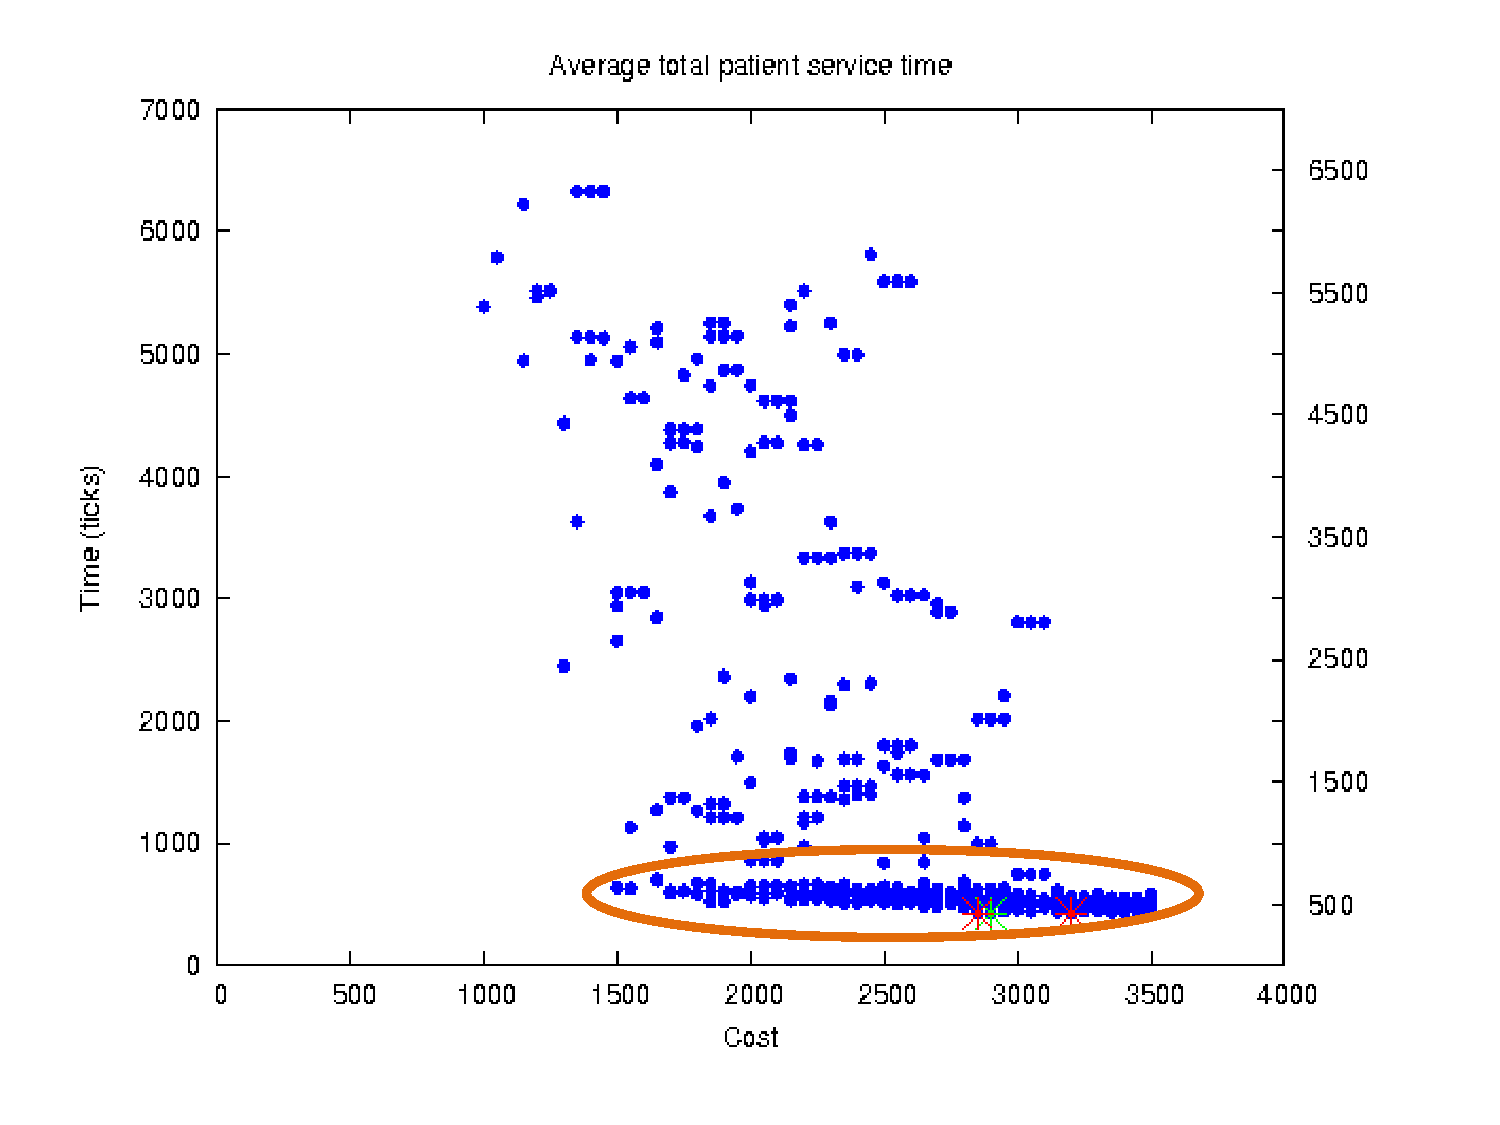
\includegraphics[width=80mm,height=51mm]{staff_cost_time_20.pdf}
                \label{subfloat:exp1_20}
            }
&
        \subfloat[][Average minimum LoS with P = 80\%.] {
                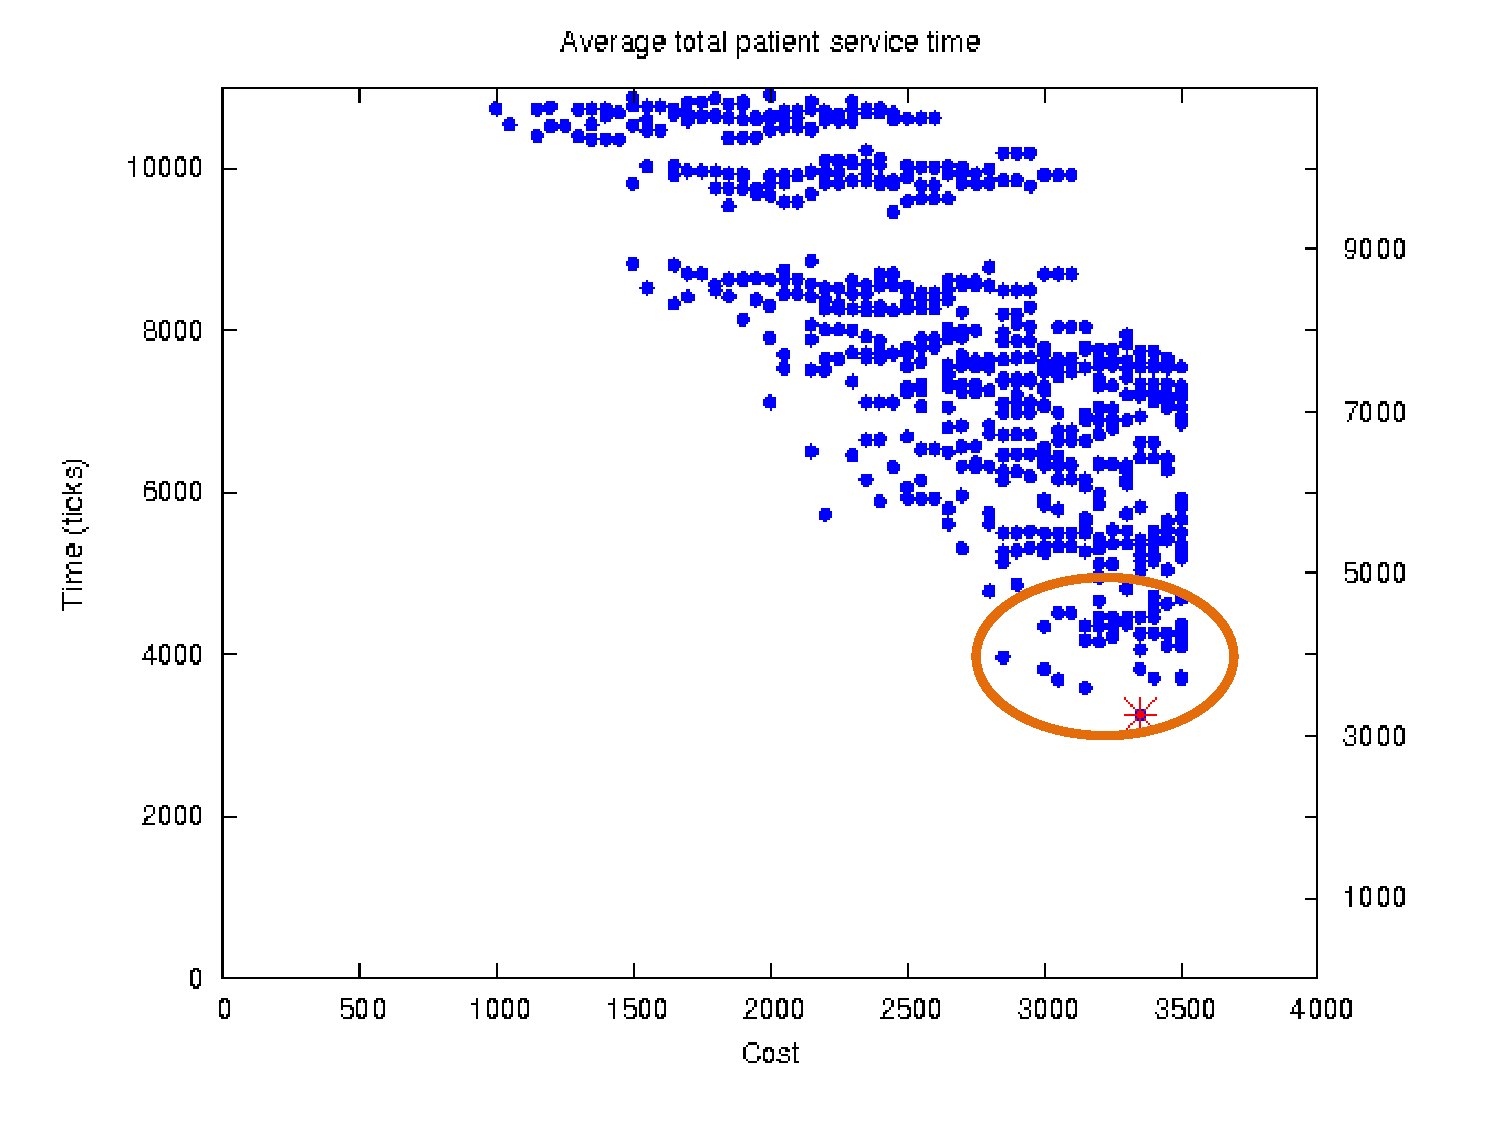
\includegraphics[width=80mm,height=51mm]{staff_cost_time_80.pdf}
                \label{subfloat:exp1_80}
        }
	
\end{tabular}
\caption{The blue rounded points are the staff configurations that satisfy the constraint cost. Staff configurations that got the average minimum LoS are shown as green and red asterisks.}
\label{fig:exp1_20_80}
\end{figure}


From Figure \ref{subfloat:exp1_20}, it can be seen that there are three different staff configurations which obtain the minimum LoS, 
but with different costs. Also, in the same Figure \ref{subfloat:exp1_20}, it can be seen that there are many other staff 
configurations that are quite close to the minimum LoS, but with less cost. 

\begin{table}[htb!]
\centering
\caption{Staff members with their associated salary and time according to their kind, and the maximum quantity of them.}
\resizebox{2.8in}{!} {
\begin{tabular}{ccccccc}
\hline
\bf {Min}  & \bf {\euro} & \bf {Time (ticks)}  & \bf {\# staff} & \bf {D}  & \bf {N} & \bf {A}  \\ \hline
1 & 3,200 & 428 & 5 & 2 S  & 2 S  & 1 S  \\ \hline
2 & 2,900 & 428 & 5 & 2 S  & 1 S  & 2 S  \\ \hline
3 & 2,850 & 428 & 5 & 2 S  & 1 S  & 1 S, 1 J  \\ \hline
\end{tabular}
}
\label{tab:T2}
\end{table}


\begin{table}[htb!]
\centering
\caption{Staff members with their associated salary and time according to their kind, and the maximum quantity of them.}
\resizebox{2.8in}{!} {
\begin{tabular}{ccccccc}
\hline
\bf {Min}  & \bf {\euro} & \bf {Time (ticks)}  & \bf {\# staff} & \bf {D}  & \bf {N} & \bf {A}  \\ \hline
1 & 3,350 & 3,266 & 7 & 1 S, 3 J  & 2 J  & 1 J  \\ \hline
\end{tabular}
}
\label{tab:T3}
\end{table}

In the other cases, where the patient arrival increases, i.e., has higher probability (P), there are only a few staff configurations 
around the minimum, or clearly only one. Not only does the patient arrival increase, but also the minimum average patient LoS, as 
expected, as well as the cost of the staff configuration, and also the standard deviation of the average patient LoS. The amount of 
patients increases at waiting rooms, both WR1 and WR2 at times t1, t2, t3, and t4 (each time represents every 6,000 ticks of 
simulation), and finally the amount of unattended patients increases as well. In Table \ref{tab:20_80_I1} all these results are shown. 
Comparing standard deviation results show us that the variability of LoS increases as the  patient arrival P increases, but such 
variability is not linear. It is noticed that when the patient arrival P is high, 80\%, patients in waiting rooms WR1 and WR2 increase, 
i.e., the ED become overcrowded. 

\begin{table}[htb!]
\caption{Results for the best average minimum LoS for each of the four considered scenarios.}
\small\addtolength{\tabcolsep}{-5pt}
\centering
\resizebox{3.6in}{!} {
%\begin{center}
\begin{tabular}{cccccccc}
\hline
\multicolumn{ 1}{c}{\bf {P}} & \multicolumn{ 1}{c}{\bf {T1} } & \multicolumn{ 1}{c}{ \bf {$\sigma_{T1}$} } & \multicolumn{ 1}{c}{\bf {\euro} } & \multicolumn{ 1}{c}{\bf {\# attended} } & \multicolumn{ 1}{c}{\bf {\# unattended} } & \bf {WR1} & \bf {WR2} \\ \cline{ 7- 8}
\multicolumn{ 1}{c}{} & \multicolumn{ 1}{c}{\bf{(ticks)}} & \multicolumn{ 1}{c}{} & \multicolumn{ 1}{c}{} & \multicolumn{ 1}{c}{\bf {patients}} & \multicolumn{ 1}{c}{\bf {patients}} & \bf {t1, t2, t3, t4}  & \bf {t1, t2, t3, t4}  \\ \hline
20 & 428 & 48 (11\%)  & 2850 & 83 & 1 & 0,0,0,0  & 0,0,0,0  \\ \hline
%40 & 514 & 81.5  (15.9\%)  & 3,150 & 182 & 4 & 0,0,0,1  & 0,0,0,0  \\ \hline
%60 & 790 & 174.5 (22.1\%)  & 3,400 & 290 & 8 & 1,1,0,1  & 3,2,4,1  \\ \hline
80 & 3,266 & 1,670.4  (51.2\%)  & 3,350 & 294 & 100 & 8,19,32,43  & 12,25,37,51  \\ \hline
\end{tabular}
%\end{center}
}
\label{tab:20_80_I1}
\end{table}

It is worth pointing out that each of the plotted points were obtained running the simulator as many times as there are points, i.e., 
for each case the optimum red and green points were obtained through the exhaustive search technique, which implies that all the 
scenarios that satisfy the restrictions should be executed on the simulator. This implies a lot of computing time, even though 
parametric executions, through NetLogo's \emph{BehaviorSpace} tool were used. Therefore, when an entire and not simplified ED is 
used, the number of cases that have to be tested through exhaustive search will be very large. In order to reduce computational 
cost an intelligent search, other than exhaustive, must be used. 


%------------------------------------------------------------------------- 
\section {Two-phase Optimization}
\label{sec:mc_pipe}

Notice in Figure \ref{subfloat:exp1_20} and  its corresponding Table \ref{tab:T2} that there are different staff configurations that 
attained the average minimum LoS, but with different costs, as well as that there are many other staff scenarios that are quite close 
to the minimum time, but with less cost, i.e., these other solutions are sub-optimal. On the other hand, where the patient arrival 
increases, there are only a few staff configurations around the minimum, as can be seen in Figure \ref{subfloat:exp1_80} and  Table 
\ref{tab:T3}. Taking these results into account, i.e., there exist several configurations lying nearby the region where the optimum is; 
such configurations or scenarios are located inside the red ellipses in Figures \ref{subfloat:exp1_20} and  \ref{subfloat:exp1_80}. 
The red ellipses delimits a region, which is not only where the optimum is, but also where sub-optima can be found, and some of such 
sub-optima could be selected instead of the optimum with a little less LoS, but with  cheaper cost.

It was identified that ordering simulation points (ordered by ticks or weighted pipeline time ({\bf t$^*$},  using Equation 
\eqref{eq:Pipe} and also shown in Figure  \ref{fig:pipeline} ) of staff configuration), before plotting it resembles the operation of a 
pipeline. The ordered and non-ordered data are shown in Table \ref{tab:doc_ord} (similar tables were obtained for nurses, and 
admission personnel). Thus, a computationally simplified model of ED as a pipeline scheme was implemented in order to verify this 
assumption. The pipeline scheme proposed is described as follows: patients continue arriving to the service, when only one admission 
personnel, nurse and doctor are available; therefore, the ED can be seen as a single queue system, whereas when more than one 
staff is available, patients are served as if they are in many parallel servers. When the pipeline is full, i.e., all sanitarian staff 
(admission personnel, nurses and doctors are busy ) and the previous queues of triage and diagnostic are occupied, then every 
certain ticks one patient leaves the ED (ideally, because it depends on patient's acuity). 

MC is used in similar way, but in this case a specific staff configuration is selected to be tested and verified if it is the optimum; 
whereas the number of combination of EDs' staff  is increased the standard error is reduced, i.e., it is closer to the optimum in the 
region nearby.

Therefore, the proposal is to use a computationally simplified model of ED which consists of: a) pipelines, i.e., the ED can be viewed 
as a set of pipelines connected among them, and  b) MC technique in order to identify the limited region where the optimum lies. This 
can be observed in Figure \ref{fig:pipeline}. These alternative schemes to find the optimum, or the region where the optimum is, can 
lead us to find the optimum or sub-optimum values using an intelligent strategy, reducing the computing time and the region where 
the optimum lies. Once the region has been found using this scheme, the Agent-Based ED simulator previously described can be 
executed exhaustively on such a reduced region.


\begin{figure}[htb!]
{\centering {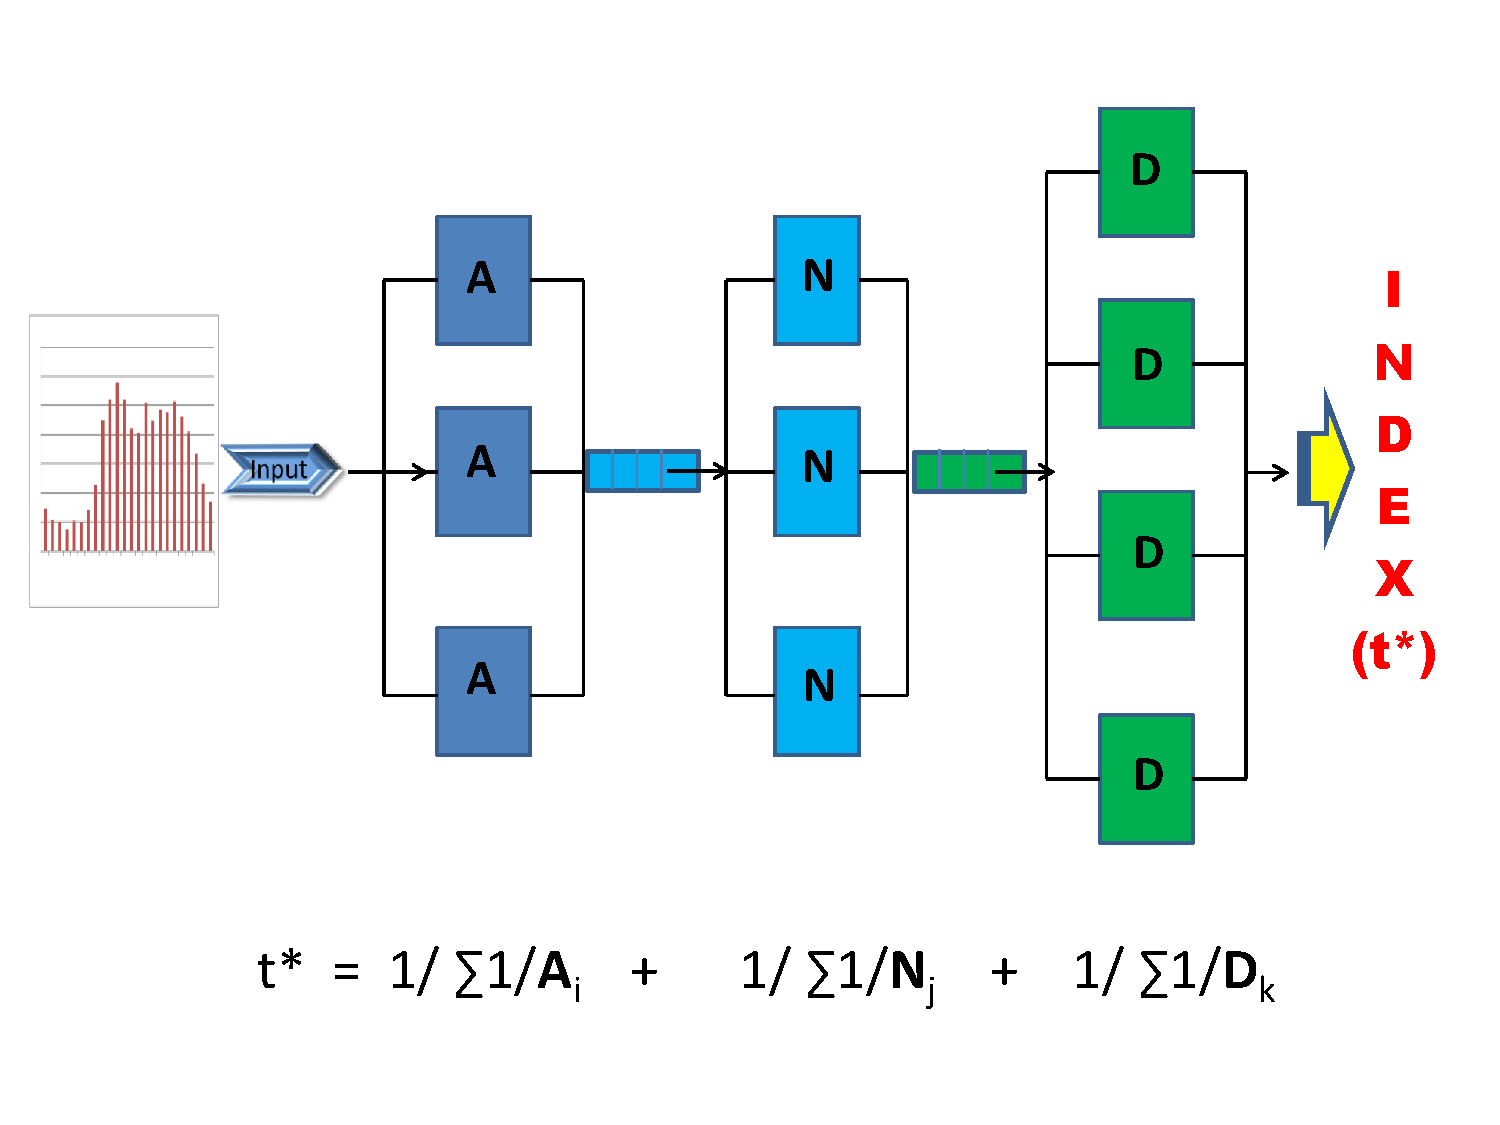
\includegraphics[width=115mm,height=38mm]{as_pipeline.pdf}}\par}
\caption{The proposal pipeline ED computationally simplified.}
\label{fig:pipeline}
\end{figure}

In  Figure \ref{fig:w_out_order}, a scattered 3D graph of the Figure \ref{subfloat:exp1_20} is shown. From this graph nothing can 
be concluded about a region where the optimum and sub-optimum are, while the same data but previously ordered according to the 
first column of the  Table \ref{tab:doc_ord} and obtained through the computationally simplified proposed model of ED, Pipeline 
scheme, is shown in the Figures \ref{fig:3d_ordered} and \ref{fig:region_pipe}. In these graphs a region, where the optimum and 
sub-optima are, is clearly identified, specially in the latter, which isosurfaces are shown. In this region an exhaustive but reduced 
search is done, in order to find out the optimum using an intelligent strategy. Similar regions are found using MC scheme. 

\begin{table}[htb!]
\caption{Ordering data according to working time of each staff configuration of Doctors.}
\begin{center}
\resizebox{3.8in}{!}  {
\begin{tabular}{ccccccccc}
\hline
\bf {Ordered t$^*$ } &  \bf {Non ordered} & \bf {DR$_1$} & \bf {DR$_2$} & \bf {DR$_3$} & \bf {DR$_4$} & \bf {\euro} & \bf {t(ticks)}  &  \bf {t$^*$ (ticks)}  \\ \hline
1 & 10& DS & DS & DS & DS & 4,000 & 260 & 65  \\ \hline
2 & 14& DS & DS & DS & DJ & 3,500 & 350 & 69.5  \\ \hline
3 & 13& DS & DS & DJ & DJ & 3,000 & 350 & 74.6  \\ \hline
4 & 12& DS & DJ & DJ & DJ & 2,500 & 350 & 80.5  \\ \hline
5 & 6& DS & DS & DS & -  & 3,000 & 260 & 86.7  \\ \hline
6 & 11& DJ & DJ & DJ & DJ & 2,000 & 350 & 87.5  \\ \hline
7 & 9& DS & DS & DJ & - & 2,500 & 350 & 94.8  \\ \hline
8 & 8& DS & DJ & DJ & - & 2,000 & 350 & 104.6  \\ \hline
9 & 7& DJ & DJ & DJ & - & 1,500 & 350 & 116.7  \\ \hline
10 & 3& DS & DS & - & - & 2,000 & 260 & 130  \\ \hline
11 & 5& DS & DJ & - & - & 1,500 & 350 & 149  \\ \hline
12 & 4& DJ & DJ & - & - & 1,000 & 350 & 175  \\ \hline
13 & 1& DS & -  & - & -& 1,000 & 260 & 260  \\ \hline
14 & 2& DJ & -  & - & -  & 500 & 350 & 350  \\ \hline
\end{tabular}
}
\end{center}
\label{tab:doc_ord}
\end{table}

\begin{figure}[htb!]
{\centering {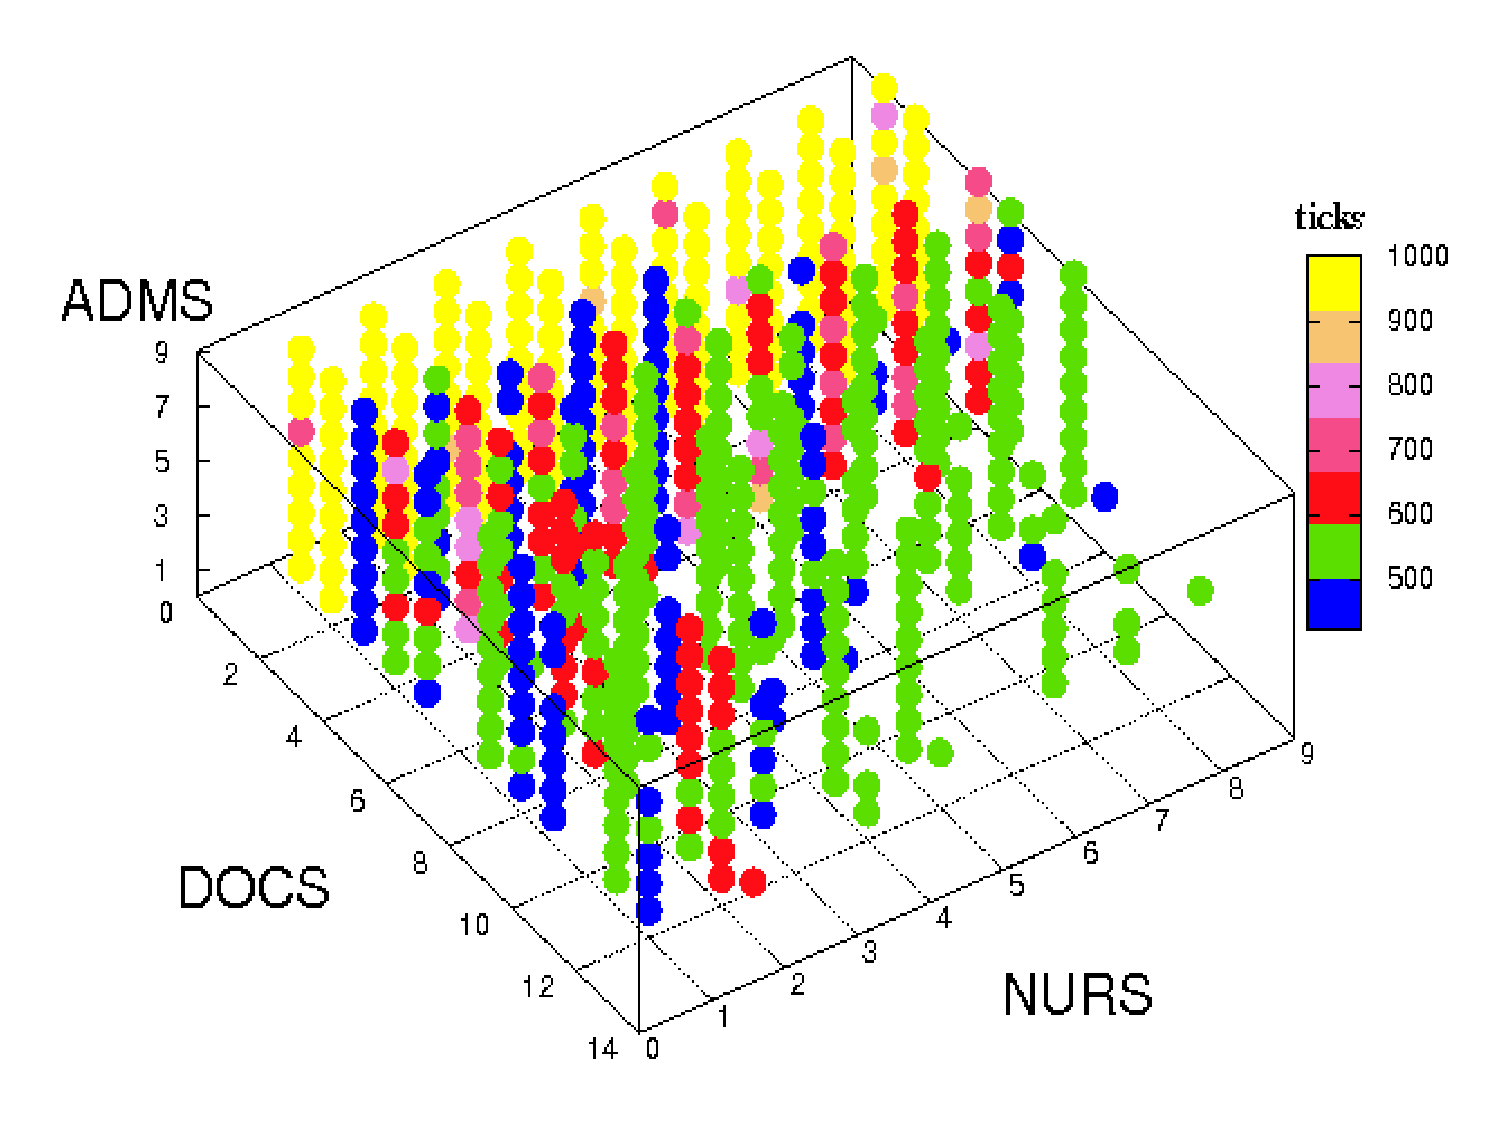
\includegraphics[width=130mm,height=42mm]{3d_woorder.pdf}}\par}
\caption{Scattered  3D graph using the second column of the Table  \ref{tab:doc_ord} where there is a lack of order of staff configuration. The axes are labeled by the number of combinations of each ED staff: up to 9 for Nurses and Admission personnel and up to 14 for Doctors.}
\label{fig:w_out_order}
\end{figure}

\begin{figure}[htb!]
{\centering {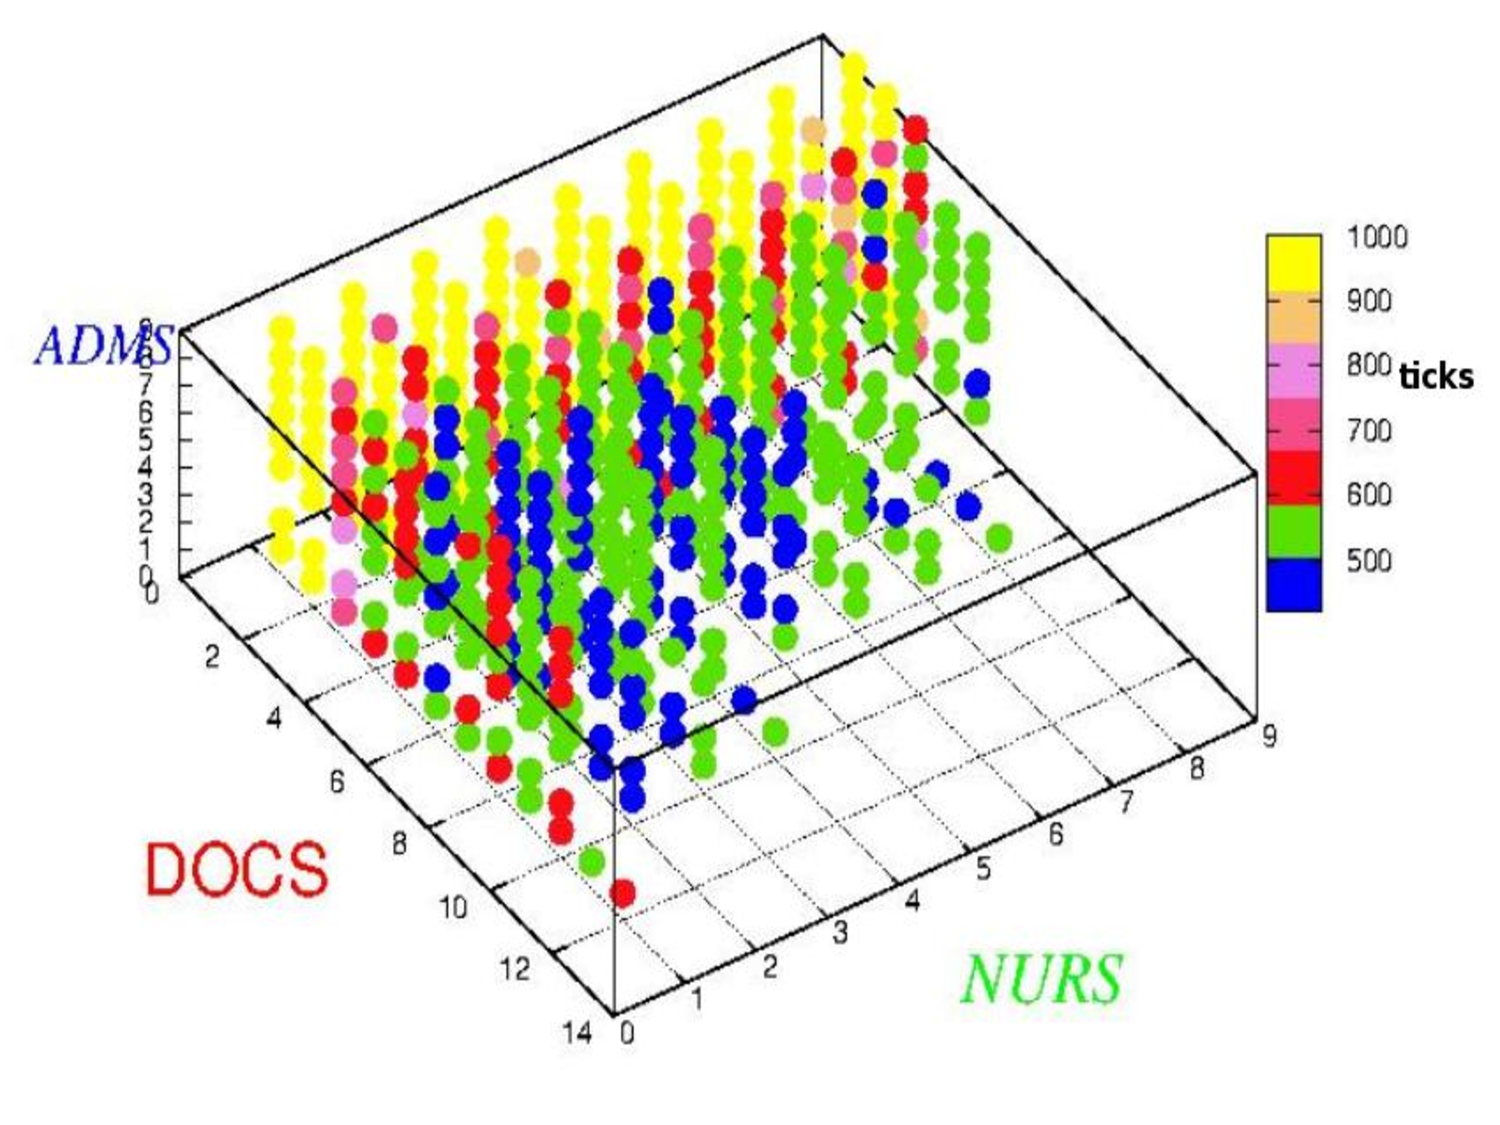
\includegraphics[width=130mm,height=42mm]{3d_ordered.pdf}}\par}
\caption{Scattered  3D graph obtained through the proposed reduce ordered  scheme Pipeline. The axes are labeled by the number of combinations of each ED staff: up to 9 for Nurses and Admission personnel and up to 14 for Doctors.}
\label{fig:3d_ordered}
\end{figure}

\begin{figure}[htb!]
{\centering {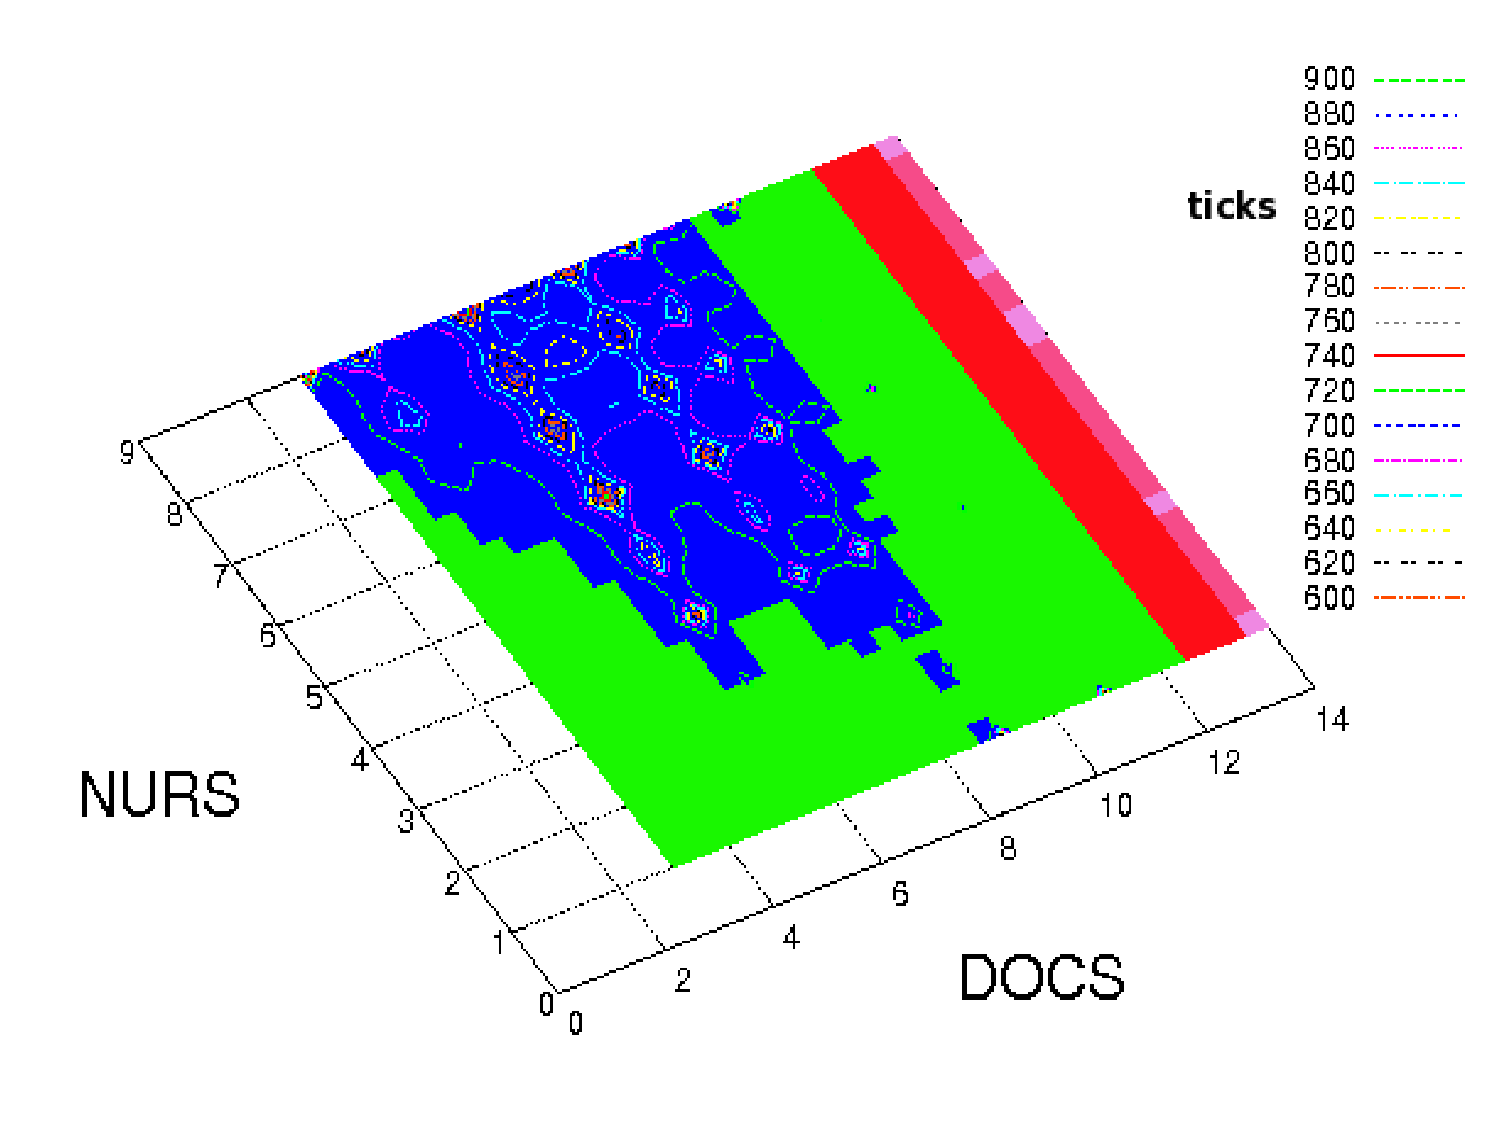
\includegraphics[width=130mm,height=42mm]{ordered_tpipe_pm3d_contour.pdf}}\par}
\caption{Isosurfaces graph obtained through the proposed ordered reduce scheme Pipeline. The axes are labeled by the number of combinations of each ED staff: up to 9 for Nurses and Admission personnel and up to 14 for Doctors.}
\label{fig:region_pipe}
\end{figure}



\section{Introduction}

The two-phase optimisation via simulation of healthcare Emergency
Departments, ED, proposed in \ref{ch3:Proposed-OvS-ED} was applied
herewith to analyse the administrative strategies leading to optimum
decisions about the physical and human resources of an ED. In particular,
the impact on the economics and the productivity of Sabadell Hospital
ED of different sanitary staff configuration (v.gr., doctors, triage
nurses, admission personnel, emergency nurses, and x-ray technicians)
were analysed. It is a discrete combinatorial optimisation problem.

There are three main issues to be addressed to carry out the evaluation,
namely: the \textit{simulation models} that represent the system under
study (discussed along the previous chapters); the \textit{decision
variables} and\textit{ workloads} used as inputs of the simulation
models; and the \textit{metrics} used to asses the benefits of the
proposal. We have defined some significant workloads and a set of
metrics to observe both functional and performance features of the
proposal. This set of metrics were defined in term of three different
indexes, namely: patient length of stay (LoS) in the ED; number of
attended patients per day (Throughput); and a compound index, the
product of the cost of a given sanitary staff configuration times
patient length of stay (CLoS).

In the following sections, the \textit{decision variables, }the\textit{
workloads}, and the \textit{metrics} are described. Finally two case
scenarios and their results are presented and discussed. 


\section{Field Information of Sabadell Hospital ED}

It was found through interviews with the managers at the EDs of Sabadell
hospital (which provides healthcare services to an average of 160,000
patients/year), it was found that a basic sanitary of its ED staff
is composed by: doctors, triage nurses, emergency nurses, admission
personnel, and x-ray technicians, as shown in \ref{tab:T1}. This
table also shows some characteristics of such sanitary staff, namely:
sort of staff as junior or senior (that represents less and more expertise,
respectively); their respective costs (� \textbf{}%
\footnote{\textbf{It is not an actual euro, could be any currency.\label{fn:euro}}%
}); the operational patient-service-time (hours); and the minimum and
maximum number of each kind of staff. 

\begin{comment}
 %
\saveFN\mymark  %
\end{comment}
\foreignlanguage{american}{}%
\begin{comment}
 %
\useFN\mymark  %
\end{comment}


\begin{table}[H]
\caption{Sabadell Hospital ED staff and their: associated expertise, costs,
operational patient-service time, and number.}


\begin{centering}
\begin{tabular}{>{\centering}m{3.5cm}>{\centering}p{1.1cm}>{\centering}p{1cm}>{\centering}p{1.1cm}>{\centering}p{1cm}>{\centering}m{0.075cm}>{\centering}m{2.2cm}}
\cline{1-5} \cline{7-7} 
\multicolumn{1}{>{\centering}m{3.5cm}|}{\textbf{Sanitary staff} } & \multicolumn{2}{c|}{\textbf{Cost (�$^{1}$)}} & \multicolumn{2}{c}{\textbf{Time/patient (hours)}} &  & \textbf{Number of personnel}\tabularnewline
\cline{1-5} \cline{7-7} 
 & Senior  & Junior  & Senior & Junior &  & min - Max\tabularnewline
\cline{1-5} \cline{7-7} 
Doctor  & 1000  & 500  & 0.26 & 0.35 &  & \textbf{\textit{1 -- 4}} \tabularnewline
\cline{1-5} \cline{7-7} 
Triage Nurse  & 500  & 350  & 0.09 & 0.13 &  & \textbf{\textit{1 -- 3}} \tabularnewline
\cline{1-5} \cline{7-7} 
Emergency Nurse & 500  & 350  & 0.14 & 0.18 &  & \textbf{\textit{1 -- 2}} \tabularnewline
\cline{1-5} \cline{7-7} 
Admission personnel & 200  & 150  & 0.02 & 0.035 &  & \textbf{\textit{1 -- 3}} \tabularnewline
\cline{1-5} \cline{7-7} 
X-ray technician & 200  & 150  & 0.09 & 0.14 &  & \textbf{\textit{1 -- 2}} \tabularnewline
\cline{1-5} \cline{7-7} 
\end{tabular}
\par\end{centering}

\label{tab:T1} 
\end{table}


\begin{figure}[H]
\centering 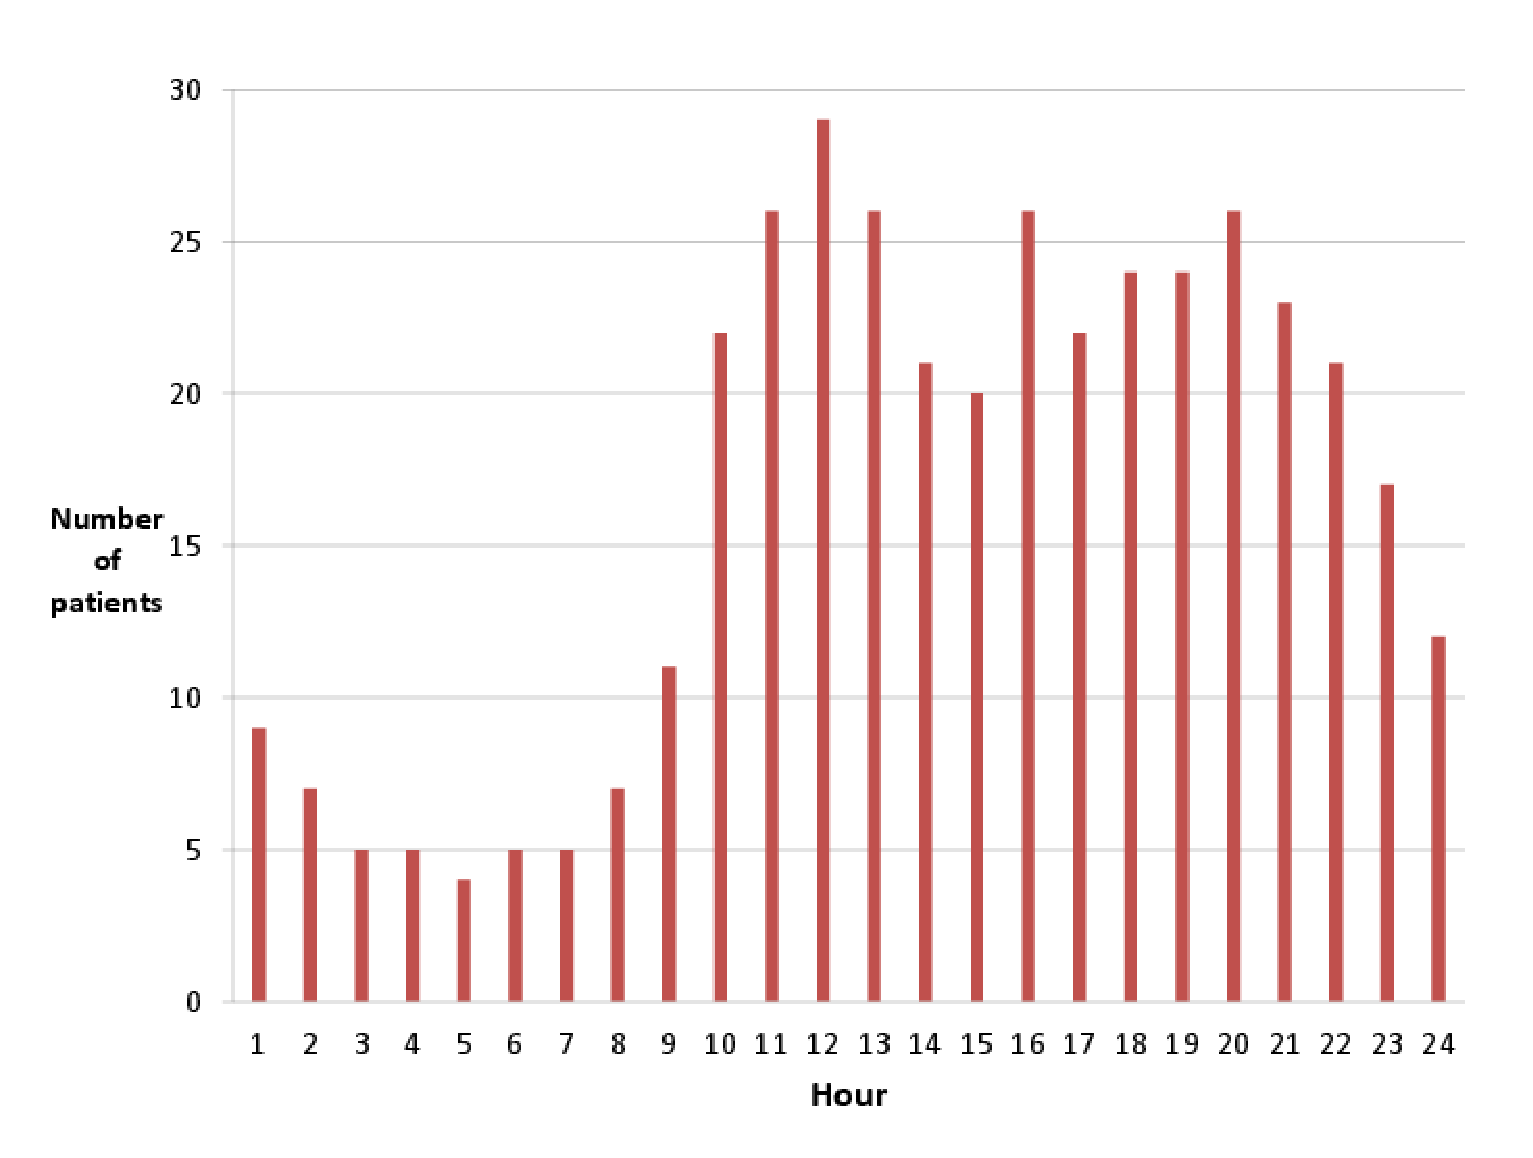
\includegraphics[width=0.85\columnwidth,height=0.17\paperheight]{figs4/input} 

\caption{Sabadell Hospital ED average of 400 daily incoming patients and its
hourly distribution (February 2010).\label{fig:real-input}}
\end{figure}


In reference to the Sabadell Hospital ED incoming patients, an average
of four hundred of patients daily arrive to the ED of Sabadell hospital.
As example, the statistics corresponding to February 2010, of this
real average number of incoming patients and its hourly distribution
are shown in \ref{fig:real-input}. As stated in \ref{sec:active-agents}
all incomings patients are triaged to identify the acuity of them
and to prioritise their urgency of attention. Thus, the average percentage,
according to the priority level of urgency of attention, of the incoming
patients to the ED of Sabadell hospital is as follows: triage level
1 - 1\%; triage level 2 - 4\%; triage level 3 - 20\%; triage level
4 - 32\%;and triage level 5 - 43\%. Patients identified as triage
level 4 and triage level 5 represent up to 75\% of the total of the
incoming patients to the ED of Sabadell hospital.

\begin{comment}
All simulations were done using the simulator previously explained,
utilising the \emph{BehaviorSpace} tool, serially and using the cluster
\textit{IBM} of the department, which has 32 Compute nodes with 2
x Dual-Core Intel(R) Xeon(R) CPU 5160 running at 3.00GHz, with 12
GB of RAM, and 4MB of L2 share cache (2x2)
\end{comment}


%\begin{figure}[htb!] 
%\centering 
%\begin{tabular}{ccc} 	
%	\subfloat[][9 Admission (A) personnel staff cases. AD\textit{i} represents Admission Den %\textit{i}.] 
%{\label{subfloat:adm_comb} 
%\resizebox{1.7in}{!} { 
%\begin{tabular}{cccc} 
%\hline 
%Case number & \bf{AD$_1$} & \bf {AD$_2$}  & \bf {AD$_3$}  \\ \hline 
%1 & AS  & -  & -    \\ \hline 
%2 & AJ  & -  & -    \\ \hline 
%3 & AS  & AS  & -    \\ \hline 
%4 & AJ  & AJ  & -    \\ \hline 
%5 & AS  & AJ  & -    \\ \hline 
%6 & AS  & AS  & AS    \\ \hline 
%7 & AJ  & AJ  & AJ    \\ \hline 
%8 & AS  & AJ  & AJ    \\ \hline 
%9 & AS  & AS  & AJ    \\ \hline 
%\end{tabular} 
%}         
%} 
%& 	
%	\subfloat[][9 Nurse (N) cases. TR\textit{i} represents Triage Room \textit{i}.] 
%{\label{subfloat:nur_comb} 
%\resizebox{1.7in}{!} { 
%\begin{tabular}{cccc} 
%\hline 
%Case number & \bf {TR$_1$} & \bf {TR$_2$}  & \bf {TR$_3$}  \\ \hline 
%1 & NS  & -  & -    \\ \hline 
%2 & NJ  & -  & -    \\ \hline 
%3 & NS  & NS  & -   \\ \hline 
%4 & NJ  & NJ  & -   \\ \hline 
%5 & NS  & NJ  & -   \\ \hline 
%6 & NS  & NS  & NS  \\ \hline 
%7 & NJ  & NJ  & NJ  \\ \hline 
%8 & NS  & NJ  & NJ  \\ \hline 
%9 & NS  & NS  & NJ  \\ \hline 
%\end{tabular} 
%}         
%} 
%&         
%	\subfloat[][14 Doctor (D) cases.  DR\textit{i} represents Diagnosis Room \textit{i}.] 
%{\label{subfloat:doc_comb} 
%\resizebox{1.99in}{!} {
%\begin{tabular}{ccccc} 
%\hline 
%Case number & \bf {DR$_1$} & \bf {DR$_2$}  & \bf {DR$_3$}  & \bf {DR$_4$}  \\ \hline 
%1 & DS  & -  & -  & -  \\ \hline 
%2 & DJ  & -  & -  & -  \\ \hline 
%3 & DS  & DS  & -  & -  \\ \hline 
%4 & DJ  & DJ  & -  & -  \\ \hline 
%5 & DS  & DJ  & -  & -  \\ \hline 
%6 & DS  & DS  & DS  & -  \\ \hline 
%7 & DJ  & DJ  & DJ  & -  \\ \hline 
%8 & DS  & DJ  & DJ  & -  \\ \hline 
%9 & DS  & DS  & DJ  & -  \\ \hline 
%10 & DS  & DS  & DS  & DS  \\ \hline 
%11 & DJ  & DJ  & DJ  & DJ  \\ \hline 
%12 & DS  & DJ  & DJ  & DJ  \\ \hline 
%13 & DS  & DS  & DJ  & DJ  \\ \hline 
%14 & DS  & DS  & DS  & DJ  \\ \hline 
%\end{tabular} 
%}       
% } 
%\end{tabular} 
%\caption{Combinations of sanitary staff: Admission (A) personnel, Nurses (N) and Doctors (D). Two levels of expertise: Junior (J), and Senior (S).} 
%\label{fig:combs} 
%\end{figure} 



\section{Decision Variables of Sabadell Hospital ED}

The sanitary staff included in \ref{tab:T1} are the \textit{decision
variables} of the ED. 
\begin{table}[H]
\noindent \begin{centering}
\hfill{}%
\begin{minipage}[t]{0.45\columnwidth}%
\centering\resizebox{2.3in}{!}{%%
\begin{tabular}{>{\centering}m{1.4cm}>{\centering}m{1.2cm}>{\centering}m{1.2cm}>{\centering}m{1.2cm}}
\hline 
Case number & \textbf{AD\textsubscript{1} } & \textbf{AD\textsubscript{2}} & \textbf{AD\textsubscript{3}}\tabularnewline
\hline 
1 & AS & - & -\tabularnewline
2 & AJ & - & -\tabularnewline
3 & AS & AS & -\tabularnewline
4 & AJ & AJ & -\tabularnewline
5 & AS & AJ & -\tabularnewline
6 & AS & AS & AS\tabularnewline
7 & AJ & AJ & AJ\tabularnewline
8 & AS & AJ & AJ\tabularnewline
9 & AS & AS & AJ\tabularnewline
\hline 
\end{tabular}}

\caption{9 Admission (A) personnel cases. AD\textit{\textsubscript{\textit{i}}}
is Admission Den\textit{\textsubscript{\textit{i}}}.$\,$Where AJ
means Admission personnel Junior, whereas AS means Admission personnel
Senior. \label{subtab:As}}
%
\end{minipage}\hfill{}%
\begin{minipage}[t]{0.45\columnwidth}%
\centering\resizebox{2.3in}{!}{%%
\begin{tabular}{>{\centering}m{1.4cm}>{\centering}m{1.2cm}>{\centering}m{1.2cm}>{\centering}m{1.2cm}}
\hline 
Case number & \textbf{TR\textsubscript{1}} & \textbf{TR\textsubscript{2}} & \textbf{TR\textsubscript{3}}\tabularnewline
\hline 
1 & NS & - & -\tabularnewline
2 & NJ & - & -\tabularnewline
3 & NS & NS & -\tabularnewline
4 & NJ & NJ & -\tabularnewline
5 & NS & NJ & -\tabularnewline
6 & NS & NS & NS\tabularnewline
7 & NJ & NJ & NJ\tabularnewline
8 & NS & NJ & NJ\tabularnewline
9 & NS & NS & NJ\tabularnewline
\hline 
\end{tabular}}

\caption{9 Nurse (N) cases. TR\textit{\textsubscript{\textit{i}}} represents
Triage Room \emph{i}. Where NJ means Triage Nurse Junior, whereas
NS means Triage Nurse Senior.\foreignlanguage{american}{\label{subtab:Ns}}}
%
\end{minipage}\hfill{}\vspace{0.1cm}

\par\end{centering}

\noindent \centering{}\hfill{}%
\begin{minipage}[t]{0.45\columnwidth}%
\centering\resizebox{1.7in}{!}{%
\begin{tabular}{>{\centering}m{1.4cm}>{\centering}m{1.4cm}>{\centering}m{1.4cm}}
\hline 
Case number & \textbf{ENR\textsubscript{1} } & \textbf{ENR\textsubscript{2}}\tabularnewline
\hline 
1 & ENS & -\tabularnewline
2 & ENJ & -\tabularnewline
3 & ENS & ENS\tabularnewline
4 & ENJ & ENJ\tabularnewline
5 & ENS & ENJ\tabularnewline
\hline 
\end{tabular}}

\caption{5 Emergency nurse (EN) cases. EN\textit{R\textsubscript{\textit{i}}}
represents ENurse Room \emph{i}. Where ENJ means Emergency Nurse Junior,
whereas ENS means Emergency Nurse Senior\foreignlanguage{american}{\label{subtab:ENs}}}
%
\end{minipage}\hfill{}%
\begin{minipage}[t]{0.45\columnwidth}%
\centering\resizebox{1.7in}{!}{%%
\begin{tabular}{>{\centering}m{1.4cm}>{\centering}m{1.4cm}>{\centering}m{1.4cm}}
\hline 
Case number & \textbf{XR\textsubscript{1}} & \textbf{XR\textsubscript{2}}\tabularnewline
\hline 
1 & XRS & -\tabularnewline
2 & XRJ & -\tabularnewline
3 & XRS & XRS\tabularnewline
4 & XRJ & XRJ\tabularnewline
5 & XRS & XRJ\tabularnewline
\hline 
\end{tabular}}

\caption{5 X-ray technician (XR) cases. XR\textit{\textsubscript{\textit{i}}}
represents X-ray Room \emph{i}. Where XRJ means X-ray technician Junior,
whereas XRS means X-ray technician Senior\foreignlanguage{american}{\label{subtab:Xrs}}}
%
\end{minipage}\hfill{}
\end{table}
 The disaggregation of \ref{tab:T1} yields \ref{subtab:As}, which
includes 9 possible combinations of admission personnel (junior/senior);
\ref{subtab:Ns}, which also includes 9 possible combinations of triage
nurses (junior/senior); \ref{subtab:ENs}, that presents the 5 possible
combinations of emergency nurse (junior/senior); \ref{subtab:Xrs}
that shows the 5 possible combinations of x-ray technician (junior/senior);
and \ref{subtab:Ds}, with 14 possible combinations of doctors (junior/senior)
in which the examined cases for each type of staff were included.
It is a discrete combinatorial problem.

 %
\begin{table}[H]
\caption{  %
14 Doctor (D) cases. DR\textit{\textsubscript{\textit{i}}} represents
Diagnosis Room \emph{i}. Where DJ means Doctor Junior, whereas DS
means Doctor Senior\foreignlanguage{american}{.\label{subtab:Ds}} %
}
\centering\resizebox{2.6in}{!}{%%
\begin{tabular}{>{\centering}m{1.4cm}>{\centering}m{1.1cm}>{\centering}m{1.1cm}>{\centering}m{1.1cm}>{\centering}m{1.1cm}}
\hline 
  %
Case number %
 &   %
\textbf{DR\textsubscript{1}} %
 &   %
\textbf{DR\textsubscript{2} } %
 &   %
\textbf{DR\textsubscript{3}} %
 &   %
\textbf{DR\textsubscript{4}} %
\tabularnewline
\hline 
  %
1 %
 &   %
DS %
 &   %
- %
 &   %
- %
 &   %
- %
\tabularnewline
  %
2 %
 &   %
DJ %
 &   %
- %
 &   %
- %
 &   %
- %
\tabularnewline
  %
3 %
 &   %
DS %
 &   %
DS %
 &   %
- %
 &   %
- %
\tabularnewline
  %
4 %
 &   %
DJ %
 &   %
DJ %
 &   %
- %
 &   %
- %
\tabularnewline
  %
5 %
 &   %
DS %
 &   %
DJ %
 &   %
- %
 &   %
- %
\tabularnewline
  %
6 %
 &   %
DS %
 &   %
DS %
 &   %
DS %
 &   %
- %
\tabularnewline
  %
7 %
 &   %
DJ %
 &   %
DJ %
 &   %
DJ %
 &   %
- %
\tabularnewline
  %
8 %
 &   %
DS %
 &   %
DJ %
 &   %
DJ %
 &   %
- %
\tabularnewline
  %
9 %
 &   %
DS %
 &   %
DS %
 &   %
DJ %
 &   %
- %
\tabularnewline
  %
10 %
 &   %
DS %
 &   %
DS %
 &   %
DS %
 &   %
DS %
\tabularnewline
  %
11 %
 &   %
DJ %
 &   %
DJ %
 &   %
DJ %
 &   %
DJ %
\tabularnewline
  %
12 %
 &   %
DS %
 &   %
DJ %
 &   %
DJ %
 &   %
DJ %
\tabularnewline
  %
13 %
 &   %
DS %
 &   %
DS %
 &   %
DJ %
 &   %
DJ %
\tabularnewline
  %
14 %
 &   %
DS %
 &   %
DS %
 &   %
DS %
 &   %
DJ %
\tabularnewline
\hline 
\end{tabular}}
\end{table}


  %
\ref{subtab:As} to \ref{subtab:Ds} were ordered by the sort and
number of staff, whereas \ref{subtab:As-pipe} to \ref{subtab:XRs-pipe}
were ordered by the equivalent operational patient-service time \foreignlanguage{american}{(t{*})}
of a ``single one'' sanitary professional (working in parallel)
of each sanitary staff configuration (admission personnel, nurses,
doctors, and x-ray technicians). This order was obtained by applying
the pipeline scheme described in \ref{sub:Pipeline-Model-ED} and
is graphically shown in \ref{fig:3D-scattered-LoS-wo} to \ref{fig:3D-scattered-LoS-tpipe}.
In these figures the index value was represented by colours, the most
important values in such figures were the green ones. 
\begin{table}[h]
 %
\caption{  %
Ordering staff configuration of admission personnel according to the
equivalent operational patient-service time \foreignlanguage{american}{(t{*})}
of each staff configuration.\label{subtab:As-pipe} %
}
\centering\resizebox{4.5in}{!}{%%
\begin{tabular}{>{\centering}m{1.4cm}>{\centering}m{1.4cm}>{\centering}m{1.2cm}>{\centering}m{1.2cm}>{\centering}m{1.2cm}>{\centering}m{1.2cm}>{\centering}m{1.2cm}>{\centering}m{1.2cm}}
\hline 
  %
Case number (t{*}) %
 &   %
Old case number %
 &   %
\textbf{AD\textsubscript{1} } %
 &   %
\textbf{AD\textsubscript{2}} %
 &   %
\textbf{AD\textsubscript{3}} %
 &   %
\textbf{�} %
 &   %
\textbf{Time (hrs)} %
 &   %
\textbf{t{*}}

\textbf{(hrs)} %
\tabularnewline
\hline 
  %
1 %
 &   %
6 %
 &   %
AS %
 &   %
AS %
 &   %
AS %
 &   %
600 %
 &   %
0.02 %
 &   %
0.007 %
\tabularnewline
  %
2 %
 &   %
9 %
 &   %
AS %
 &   %
AS %
 &   %
AJ %
 &   %
550 %
 &   %
0.035 %
 &   %
0.008 %
\tabularnewline
  %
3 %
 &   %
8 %
 &   %
AS %
 &   %
AJ %
 &   %
AJ %
 &   %
500 %
 &   %
0.035 %
 &   %
0.009 %
\tabularnewline
  %
4 %
 &   %
3 %
 &   %
AS %
 &   %
AS %
 &   %
- %
 &   %
400 %
 &   %
0.02 %
 &   %
0.001 %
\tabularnewline
  %
5 %
 &   %
7 %
 &   %
AJ %
 &   %
AJ %
 &   %
AJ %
 &   %
450 %
 &   %
0.035 %
 &   %
0.012 %
\tabularnewline
  %
6 %
 &   %
5 %
 &   %
AS %
 &   %
AJ %
 &   %
- %
 &   %
350 %
 &   %
0.035 %
 &   %
0.013 %
\tabularnewline
  %
7 %
 &   %
4 %
 &   %
AJ %
 &   %
AJ %
 &   %
- %
 &   %
300 %
 &   %
0.035 %
 &   %
0.018 %
\tabularnewline
  %
8 %
 &   %
1 %
 &   %
AS %
 &   %
- %
 &   %
- %
 &   %
200 %
 &   %
0.02 %
 &   %
0.02 %
\tabularnewline
  %
9 %
 &   %
2 %
 &   %
AJ %
 &   %
- %
 &   %
- %
 &   %
150 %
 &   %
0.035 %
 &   %
0.035 %
\tabularnewline
\hline 
\end{tabular}}  %
\end{table}
 
\begin{table}[h]
 %
\caption{  %
Ordering staff configuration of triage nurses according to the equivalent
operational patient-service time \foreignlanguage{american}{(t{*})}
of each staff configuration.\label{subtab:Ns-pipe} %
}
\centering\resizebox{4.5in}{!}{%%
\begin{tabular}{>{\centering}m{1.4cm}>{\centering}m{1.4cm}>{\centering}m{1.2cm}>{\centering}m{1.2cm}>{\centering}m{1.2cm}>{\centering}m{1.2cm}>{\centering}m{1.2cm}>{\centering}m{1.2cm}}
\hline 
  %
Case number (t{*}) %
 &   %
Old case number %
 &   %
\textbf{TR\textsubscript{1} } %
 &   %
\textbf{TR\textsubscript{2}} %
 &   %
\textbf{TR\textsubscript{3}} %
 &   %
\textbf{�} %
 &   %
\textbf{Time (hrs)} %
 &   %
\textbf{t{*}}

\textbf{(hrs)} %
\tabularnewline
\hline 
  %
1 %
 &   %
6 %
 &   %
NS %
 &   %
NS %
 &   %
NS %
 &   %
1,500 %
 &   %
0.09 %
 &   %
0.03 %
\tabularnewline
  %
2 %
 &   %
9 %
 &   %
NS %
 &   %
NS %
 &   %
NJ %
 &   %
1,350 %
 &   %
0.13 %
 &   %
0.033 %
\tabularnewline
  %
3 %
 &   %
8 %
 &   %
NS %
 &   %
NJ %
 &   %
NJ %
 &   %
1,200 %
 &   %
0.13 %
 &   %
0.04 %
\tabularnewline
  %
4 %
 &   %
7 %
 &   %
NJ %
 &   %
NJ %
 &   %
NJ %
 &   %
1,050 %
 &   %
0.13 %
 &   %
0.043 %
\tabularnewline
  %
5 %
 &   %
3 %
 &   %
NS %
 &   %
NS %
 &   %
- %
 &   %
1,000 %
 &   %
0.09 %
 &   %
0.05 %
\tabularnewline
  %
6 %
 &   %
5 %
 &   %
NS %
 &   %
NJ %
 &   %
- %
 &   %
850 %
 &   %
0.13 %
 &   %
0.053 %
\tabularnewline
  %
7 %
 &   %
4 %
 &   %
NJ %
 &   %
NJ %
 &   %
- %
 &   %
700 %
 &   %
0.13 %
 &   %
0.07 %
\tabularnewline
  %
8 %
 &   %
1 %
 &   %
NS %
 &   %
- %
 &   %
- %
 &   %
500 %
 &   %
0.09 %
 &   %
0.09 %
\tabularnewline
  %
9 %
 &   %
2 %
 &   %
NJ %
 &   %
- %
 &   %
- %
 &   %
350 %
 &   %
0.13 %
 &   %
0.13 %
\tabularnewline
\hline 
\end{tabular}}  %
\end{table}
 \foreignlanguage{american}{}
\begin{table}[H]
 %
\caption{  %
Ordering staff configuration of doctors according to the equivalent
operational patient-service time \foreignlanguage{american}{(t{*})}
of each staff configuration.\foreignlanguage{american}{\label{subtab:Ds-pipe}} %
}
\centering\resizebox{4.8in}{!}{%%
\begin{tabular}{>{\centering}m{1.4cm}>{\centering}m{1.4cm}>{\centering}m{1.1cm}>{\centering}m{1.1cm}>{\centering}m{1.1cm}>{\centering}m{1.1cm}>{\centering}m{1.1cm}>{\centering}m{1.1cm}>{\centering}m{1.5cm}}
\hline 
  %
Case number (t{*}) %
 &   %
Old case number %
 &   %
\textbf{DR\textsubscript{1}} %
 &   %
\textbf{DR\textsubscript{2}} %
 &   %
\textbf{DR\textsubscript{3}} %
 &   %
\textbf{DR\textsubscript{4}} %
 &   %
\textbf{�} %
 &   %
\textbf{Time (hrs)} %
 &   %
\textbf{t{*}}

\textbf{(hrs)} %
\tabularnewline
\hline 
  %
1 %
 &   %
10 %
 &   %
DS %
 &   %
DS %
 &   %
DS %
 &   %
DS %
 &   %
4,000 %
 &   %
0.26 %
 &   %
0.065 %
\tabularnewline
  %
2 %
 &   %
14 %
 &   %
DS %
 &   %
DS %
 &   %
DS %
 &   %
DJ %
 &   %
3,500 %
 &   %
0.35 %
 &   %
0.069 %
\tabularnewline
  %
3 %
 &   %
13 %
 &   %
DS %
 &   %
DS %
 &   %
DJ %
 &   %
DJ %
 &   %
3,000 %
 &   %
0.35 %
 &   %
0.075 %
\tabularnewline
  %
4 %
 &   %
12 %
 &   %
DS %
 &   %
DJ %
 &   %
DJ %
 &   %
DJ %
 &   %
2,500 %
 &   %
0.35 %
 &   %
0.081 %
\tabularnewline
  %
5 %
 &   %
6 %
 &   %
DS %
 &   %
DS %
 &   %
DS %
 &   %
- %
 &   %
3,000 %
 &   %
0.26 %
 &   %
0.087 %
\tabularnewline
  %
6 %
 &   %
11 %
 &   %
DJ %
 &   %
DJ %
 &   %
DJ %
 &   %
DJ %
 &   %
2,000 %
 &   %
0.35 %
 &   %
0.09 %
\tabularnewline
  %
7 %
 &   %
9 %
 &   %
DS %
 &   %
DS %
 &   %
DJ %
 &   %
- %
 &   %
2,500 %
 &   %
0.35 %
 &   %
0.095 %
\tabularnewline
  %
8 %
 &   %
8 %
 &   %
DS %
 &   %
DJ %
 &   %
DJ %
 &   %
- %
 &   %
2,000 %
 &   %
0.35 %
 &   %
0.11 %
\tabularnewline
  %
9 %
 &   %
7 %
 &   %
DJ %
 &   %
DJ %
 &   %
DJ %
 &   %
- %
 &   %
1,500 %
 &   %
0.35 %
 &   %
0.117 %
\tabularnewline
  %
10 %
 &   %
3 %
 &   %
DS %
 &   %
DS %
 &   %
- %
 &   %
- %
 &   %
2,000 %
 &   %
0.26 %
 &   %
0.13 %
\tabularnewline
  %
11 %
 &   %
5 %
 &   %
DS %
 &   %
DJ %
 &   %
- %
 &   %
- %
 &   %
1,500 %
 &   %
0.35 %
 &   %
0.149 %
\tabularnewline
  %
12 %
 &   %
4 %
 &   %
DJ %
 &   %
DJ %
 &   %
- %
 &   %
- %
 &   %
1,000 %
 &   %
0.35 %
 &   %
0.175 %
\tabularnewline
  %
13 %
 &   %
1 %
 &   %
DS %
 &   %
- %
 &   %
- %
 &   %
- %
 &   %
1,000 %
 &   %
0.26 %
 &   %
0.26 %
\tabularnewline
  %
14 %
 &   %
2 %
 &   %
DJ %
 &   %
- %
 &   %
- %
 &   %
- %
 &   %
500 %
 &   %
0.35 %
 &   %
0.35 %
\tabularnewline
\hline 
\end{tabular}}  %
\end{table}


\begin{table}[H]
 %
\caption{  %
Ordering staff configuration of emergency nurses according to the
equivalent operational patient-service time \foreignlanguage{american}{(t{*})}
of each staff configuration. \label{subtab:ENs-pipe} %
}
\centering\resizebox{3.8in}{!}{%%
\begin{tabular}{>{\centering}m{1.4cm}>{\centering}m{1.4cm}>{\centering}m{1.4cm}>{\centering}m{1.4cm}>{\centering}m{1.2cm}>{\centering}m{1.2cm}>{\centering}m{1.2cm}}
\hline 
  %
Case number (t{*}) %
 &   %
Old case number %
 &   %
\textbf{ENR\textsubscript{1}} %
 &   %
\textbf{ENR\textsubscript{2}} %
 &   %
\textbf{�} %
 &   %
\textbf{Time (hrs)} %
 &   %
\textbf{t{*}}

\textbf{(hrs)} %
\tabularnewline
\hline 
  %
1 %
 &   %
3 %
 &   %
ENS %
 &   %
ENS %
 &   %
1,000 %
 &   %
0.14 %
 &   %
0.07 %
\tabularnewline
  %
2 %
 &   %
5 %
 &   %
ENS %
 &   %
ENJ %
 &   %
850 %
 &   %
0.18 %
 &   %
0.08 %
\tabularnewline
  %
3 %
 &   %
4 %
 &   %
ENJ %
 &   %
ENJ %
 &   %
700 %
 &   %
0.18 %
 &   %
0.09 %
\tabularnewline
  %
4 %
 &   %
1 %
 &   %
ENS %
 &   %
- %
 &   %
500 %
 &   %
0.14 %
 &   %
0.14 %
\tabularnewline
  %
5 %
 &   %
2 %
 &   %
ENJ %
 &   %
- %
 &   %
350 %
 &   %
0.18 %
 &   %
0.18 %
\tabularnewline
\hline 
\end{tabular}}  %
\end{table}
 
\begin{table}[H]
 %
\caption{  %
Ordering staff configuration of x-ray technicians according to the
equivalent operational patient-service time \foreignlanguage{american}{(t{*})}
of each staff configuration.\label{subtab:XRs-pipe} %
}
\centering\resizebox{3.8in}{!}{%%
\begin{tabular}{>{\centering}m{1.4cm}>{\centering}m{1.4cm}>{\centering}m{1.2cm}>{\centering}m{1.2cm}>{\centering}m{1.2cm}>{\centering}m{1.2cm}>{\centering}m{1.2cm}}
\hline 
  %
Case number (t{*}) %
 &   %
Old case number %
 &   %
\textbf{XR\textsubscript{1} } %
 &   %
\textbf{XR\textsubscript{2}} %
 &   %
\textbf{�} %
 &   %
\textbf{Time (hrs)} %
 &   %
\textbf{t{*}}

\textbf{(hrs)} %
\tabularnewline
\hline 
  %
1 %
 &   %
3 %
 &   %
XRS %
 &   %
XRS %
 &   %
400 %
 &   %
0.09 %
 &   %
0.045 %
\tabularnewline
  %
2 %
 &   %
5 %
 &   %
XRS %
 &   %
XRJ %
 &   %
350 %
 &   %
0.14 %
 &   %
0.055 %
\tabularnewline
  %
3 %
 &   %
4 %
 &   %
XRJ %
 &   %
XRJ %
 &   %
300 %
 &   %
0.14 %
 &   %
0.07 %
\tabularnewline
  %
4 %
 &   %
1 %
 &   %
XRS %
 &   %
- %
 &   %
200 %
 &   %
0.09 %
 &   %
0.09 %
\tabularnewline
  %
5 %
 &   %
2 %
 &   %
XRJ %
 &   %
- %
 &   %
150 %
 &   %
0.14 %
 &   %
0.14 %
\tabularnewline
\hline 
\end{tabular}}  %
\end{table}
 In the first example, \ref{fig:3D-scattered-LoS-wo} shows a 3D scattered
graph, which axes were ordered by the sort and number of sanitary
staff (first column/case number of \ref{subtab:As} to \ref{subtab:Ds}.
In this graph the green points were all scattered, and they shown
lack of connectivity. 
\begin{figure}[H]
\noindent \centering{}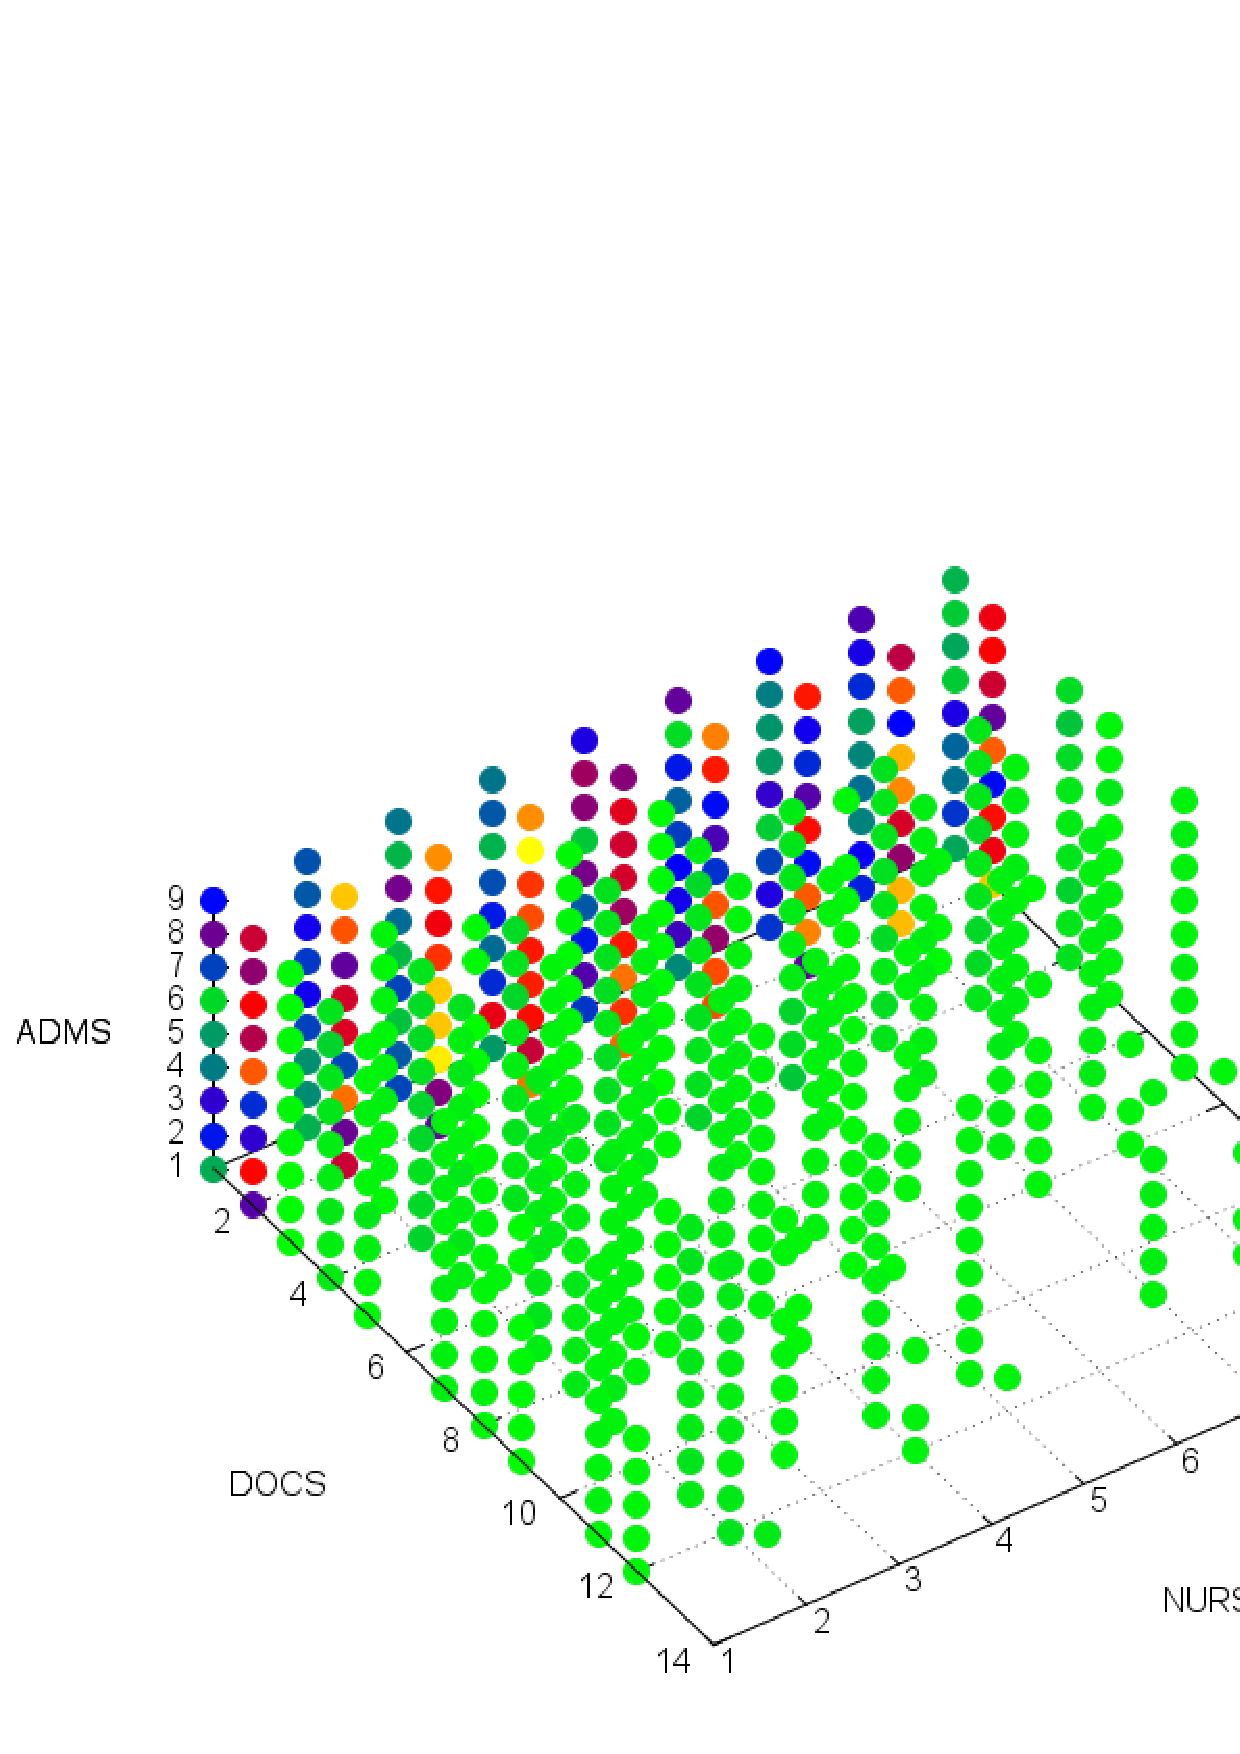
\includegraphics[width=0.88\columnwidth,height=0.2\paperheight]{figs4/3D-scatter-LoS-wo2}\caption{3D scattered graph ordered by the sort and number of staff \ref{subtab:As}
to \ref{subtab:Ds}. The green values of interest were totally scattered.
\label{fig:3D-scattered-LoS-wo}}
\end{figure}
 The second example, \ref{fig:3D-scattered-LoS-cost} shows the index
value ordered by the cost of the sanitary staff configuration. The
green points were less scattered, but blue values and others were
mixed, showing a region not totally connected. Finally, the third
example, \ref{fig:3D-scattered-LoS-tpipe}, shows the index value
ordered by the equivalent operational patient-service time \foreignlanguage{american}{(t{*})}
of each sanitary staff configuration of \ref{subtab:As-pipe} to \ref{subtab:XRs-pipe}.
This graph shows a connected and almost ``non'' scattered green
region. %
\begin{comment}
As a result of using this equivalent operational patient-service time
\foreignlanguage{american}{(t{*})} order of each staff configuration
the axes were unique and in ascending order. 
\end{comment}


\begin{figure}[h]
\noindent \begin{centering}
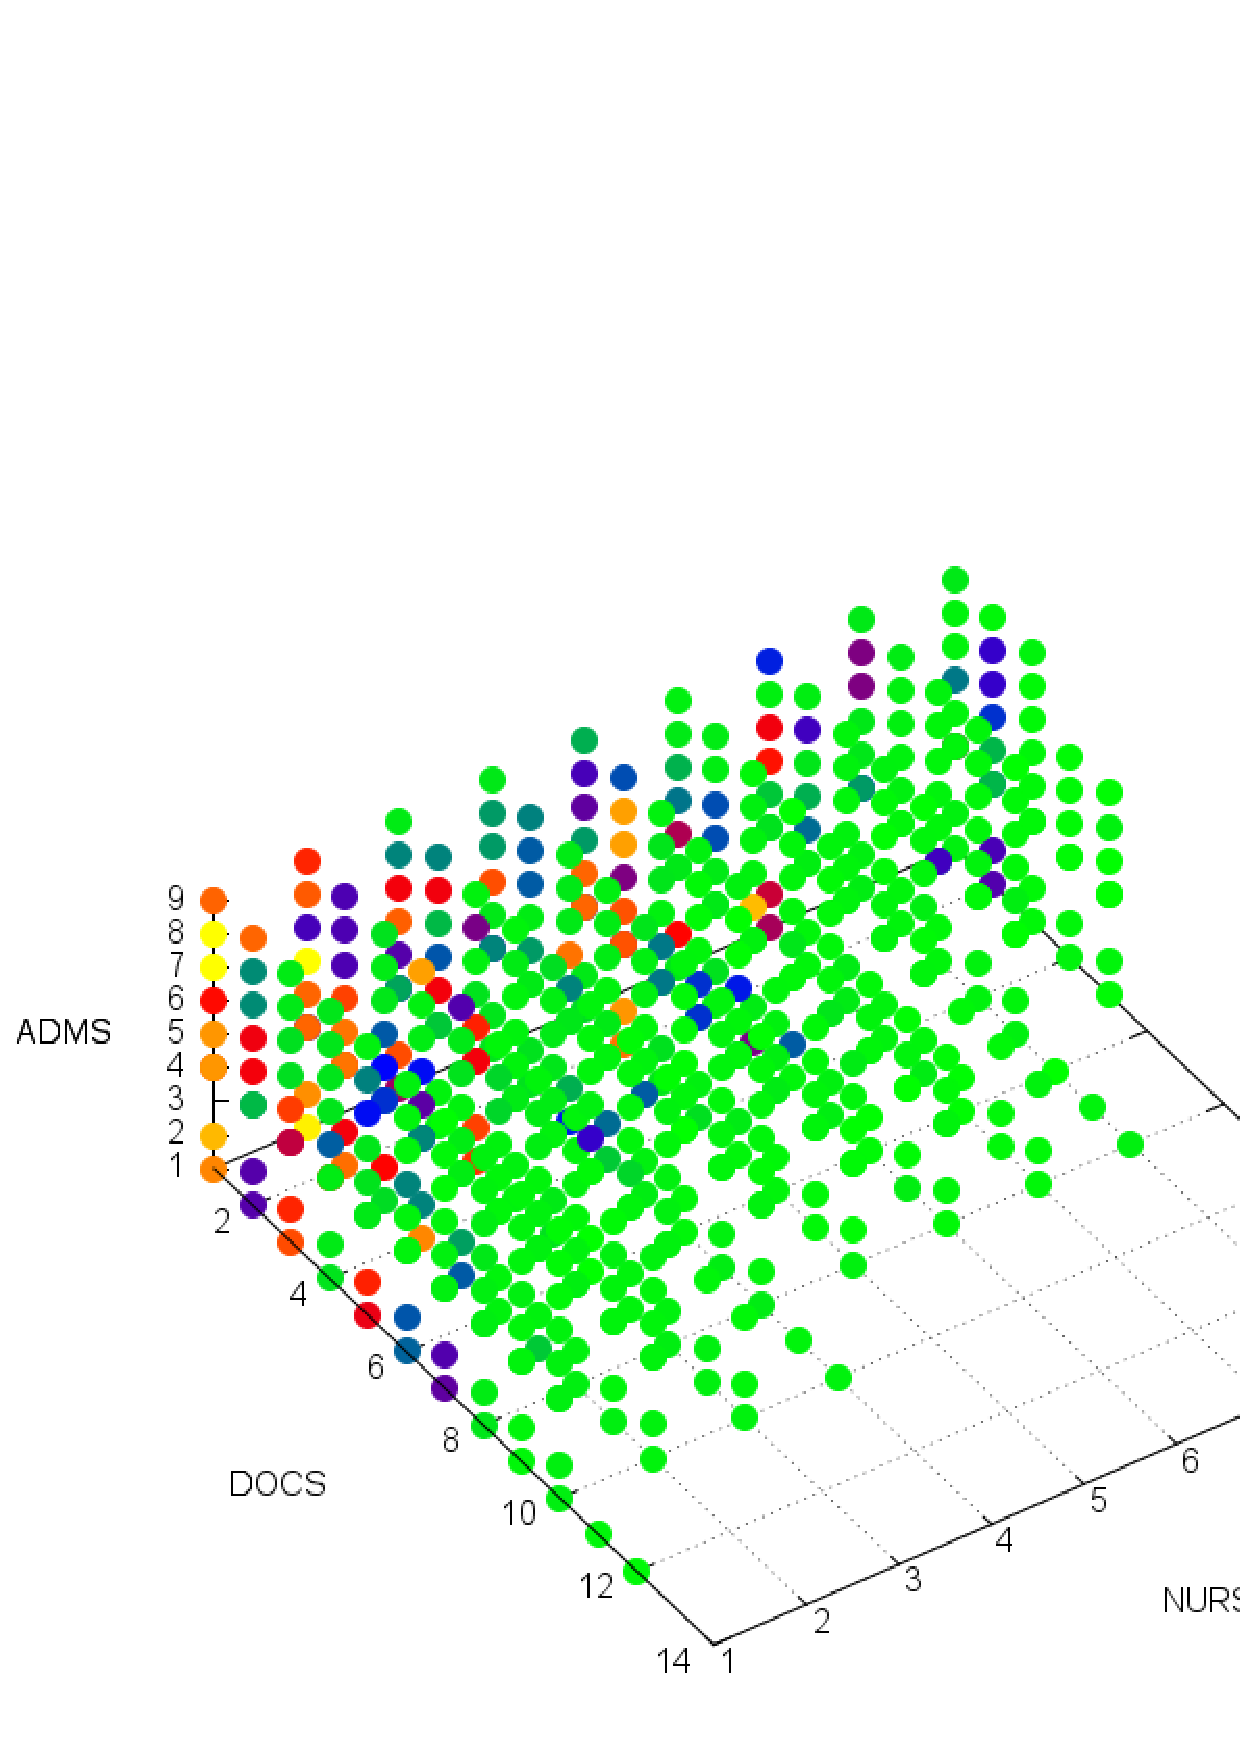
\includegraphics[width=0.88\columnwidth,height=0.2\paperheight]{figs4/3D-scatter-LoS-$2}
\par\end{centering}

\caption{3D scattered graph ordered by the cost of sanitary staff configuration.
The green values of interest were not so scattered, but not interconnected.\label{fig:3D-scattered-LoS-cost} }


\end{figure}



\section{Workloads}

In order to analyse the performance of the ED, the real average four
hundred incoming patients daily arrive to the ED of Sabadell hospital
was considered as follows. This real input was divided into four scenarios,
i.e., four different workload scenarios, up to: 4, 9, 13, and 17 incoming
patients hourly, as shown in \ref{tab:scenarios} (i.e., up to 96,
216, 312, and 408, respectively for 24hrs.).
\begin{figure}[H]
 %
\noindent \begin{centering}
\centering\foreignlanguage{british}{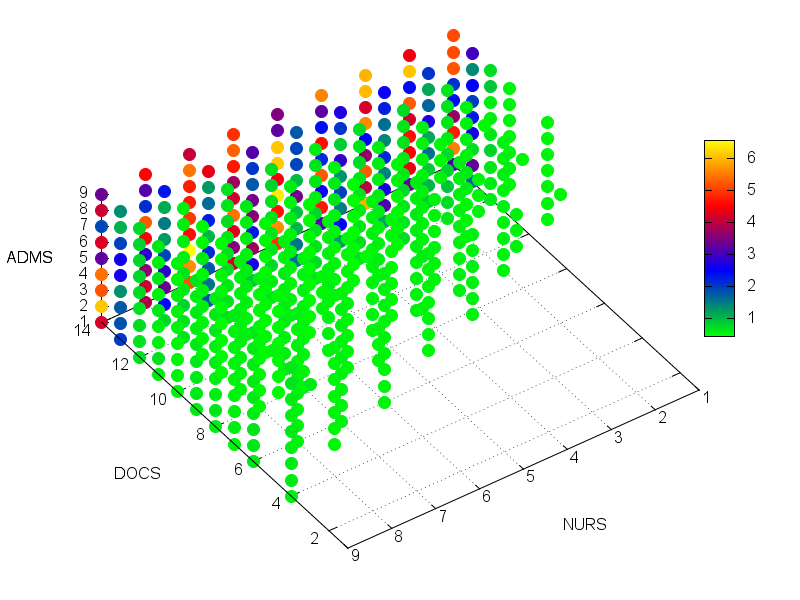
\includegraphics[width=0.88\columnwidth,height=0.2\paperheight]{figs4/3D-scatter-LoS-tpipe2}}
\par\end{centering}

  %
\caption{3D scattered graph ordered by the equivalent operational patient-service
time \foreignlanguage{american}{(t{*})} of a ``single one'' sanitary
professional of each sanitary staff configuration \ref{subtab:As-pipe}
to \ref{subtab:XRs-pipe}. The green value region of interest was
connected and almost ``non'' scattered.\label{fig:3D-scattered-LoS-tpipe} }
\end{figure}
 These different workload scenarios were used to supply different
loads to the ED, whereas the percentage of the priority level of patients
was maintained. 

\begin{table}[H]
\centering{}\caption{Incoming ED patients divided into four different workload scenarios,
up to: 4, 9, 13, and 17 patients per hour for each scenario. \label{tab:scenarios}}
\resizebox{2.3in}{!}{ %
\begin{tabular}{>{\centering}m{3.7cm}>{\centering}m{3.75cm}}
\hline 
Workload scenario number & \textbf{Incoming patients (hourly)} \tabularnewline
\hline 
1 & 4\tabularnewline
2 & 9\tabularnewline
3 & 13\tabularnewline
4 & 17\tabularnewline
\hline 
\end{tabular}}
\end{table}
\clearpage{}


\section{Evaluation Metrics}

The set of metrics used in this work were: the length of stay (LoS)
of the patients in the ED; the number of attended patients per day
(Throughput); and a compound index, the product of the cost of a given
sanitary staff configuration times patient length of stay (CLoS).

Furthermore, the computing time of each of the proposed optimisation
method is measured in order to observe the gains in reducing computing
time of the methodology proposed.\\


All simulations of the ED optimization cases analysed in this work
were carried out in a Linux cluster of the CAOS Department of the
UAB, which has 608 computing cores and 2.2TB of RAM, that is composed
of: 9 nodes of a dual-4 core Intel Xeon E5430, 2.6GHz, 16GB RAM; 1
node of 2xdual-6 core Intel Xeon E5645, 2.4GHz, 24GB RAM; and 8 nodes
of 4x16-cores AMD Opteron ``Interlagos'', 1.66GHz, 256 GB RAM, all
in a switched 1GigE network.


\section{Evaluation Method}

The evaluation of the proposed methodology was aimed to confirm the
correct operation of both the pipeline approach (PA) and the MC plus
the K-means methods, described in \ref{chap3:Math}. To this end,
we have first performed the exhaustive search (ES) to use as baseline
method. The second step of this evaluation consists on applying the
coarse grained phase, using either the PA, the MC plus K-means methods,
or both. Finally, the fine grained phase is apply in the promising
regions found in the previous step. 

In order to evaluate quantitatively the proposal methodology two case
studies were set. The first of them, namely case study A, was performed
using the agent-based ED simulator version 1.1. This case study is
further described in \ref{sub:Case-Study-A}. The second case or case
study B was performed using the agent-based ED simulator version 1.2
(the current version). This case study is further described in \ref{sub:Case-Study-B}.

In both case studies, only patients identified as triage level 4 and
5 are served at the stage of diagnosis-treatment phase, the three
metrics, and the four different workloads stated above were tested,
and the period simulated was 24 hrs., i.e., one day of functioning
of the ED, in all the experiments. Test scenarios and evaluation results
of both case studies are explained in detail in the following sections.\\


It is important to remind that the actions and interactions corresponding
to the admission and triage processes have been totally implemented,
but in the case of diagnostic and treatment phase, respecting to the
priorities of the Sabadell Hospital ED currently only the level 1
was implemented. In such level 1 only patients identified with priority
level 4 or 5 (less urgent, and non-urgent, respectively \ref{sec:active-agents})
were taken care of. Nevertheless, all incoming patients were triaged.
Once patients have been triaged, only patients identified as triage
level 4 and 5 were served at the stage of diagnosis-treatment phase.

\begin{comment}
In order to ensure the statistical value of the experiments performed,
it was necessary to execute multiple instances of the simulation with
varying random number seeds. As a rule of thumb, between two to three
tens of runs of a simulation with different random number seeds should
provide enough data to build a useful confidence interval around the
simulation results \cite{Stevens:1986}. Therefore, the simulation
model should be evaluated several times using different random seeds,
and the results obtained in such individuals simulations should be
combined in some way, v.gr., by using their average values, in order
to estimate a typical behaviour of the system. Thus, it avoids erroneous
and inaccurate analysis of the results allowing a greater degree of
confidence. 

The following two case studies presented have been conducted taking
into account the above stated issues for statistical validity. Evaluation
results and test scenarios of both case studies are explained in detail
in the following subsections.
\end{comment}



\section{Case Study A \label{sub:Case-Study-A}}

The agent-based ED simulator version 1.1, which is shown in \ref{fig:ED-SIM-0},
was used in this case study. In this version of the ED simulator the
diagnostic and treatment phase is only addressed by doctors. 
\begin{figure}[h]
\noindent \begin{centering}
\centering 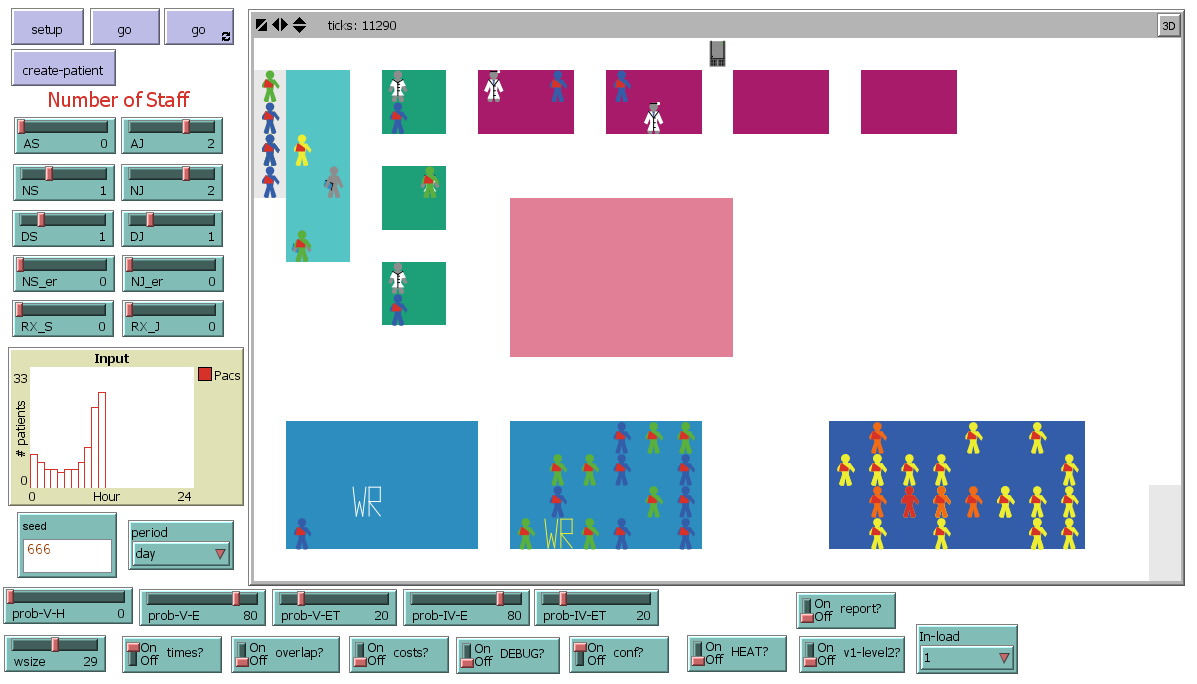
\includegraphics[width=0.9\columnwidth,height=0.16\paperheight]{figs2/ED_Netlogo-0}
\par\end{centering}

\noindent \caption{ED simulator v1.1. Admission personnel, triage nurses, and doctors
were the sanitary staff considered.}


\label{fig:ED-SIM-0} 
\end{figure}
 The simple patient flow in this ED simulator is defined as follows:
patients arrive to the ED on their own, and waits to be attended in
the admission area. Then, patients stay in the first Waiting Room
(WR) WR1, until a triage nurse call them. After the triage process
patients identified as triage level 4 and triage level 5 pass to a
second WR2, and stay there until a free doctor calls them to begin
the diagnosis-treatment phase, depending on the patient's symptoms,
physical condition, and prescribed diagnosis tests. Finally, patients
are discharged from the ED. 

Therefore, in this case study the sanitary staff considered were:
doctors, triage nurses, and admission personnel. Thus, only \ref{subtab:As}
to \ref{subtab:Ds} were taken into account. As a result, 1,134 ($14D*9N*9A$)
staff configurations were tested for each of the four workload scenarios
of incoming patients stated in \ref{tab:scenarios}. 

Finally, the three metrics above stated: LoS, Throughput, and CLoS
were obtained by applying: the ES technique; the coarse grained phase,
using both the PA and the MC plus K-means methods; then, the fine
grained phase was applied in the reduced feasible region to find the
optimum.

\begin{comment}
se han aplicado t�cnicas de paralelizaci�n. Las 4.851 configuraciones
de cada uno de los escenarios de ejecuci�n14 han sido distribuidas
entre 32 procesadores, manteniendo dicha distribuci�n en los 12 escenarios
para as� facilitar la integraci�n y tratamiento posterior de la informaci�n
de salida de las configuraciones. 
\end{comment}
\begin{comment}
\begin{figure}[h]
\hfill{}%
\begin{minipage}[c]{0.45\columnwidth}%
\includegraphics[width=1\columnwidth]{figs4/input.pdf}\caption{}
%
\end{minipage}\hfill{}%
\begin{minipage}[c]{0.45\columnwidth}%
\begin{center}
\resizebox{1.8in}{!}{ %
\begin{tabular}{>{\centering}m{1.5cm}>{\centering}m{1.75cm}}
\hline 
Scenario number & \textbf{Incoming patients (hourly)} \tabularnewline
\hline 
1 & 4\tabularnewline
\hline 
2 & 8\tabularnewline
\hline 
3 & 13\tabularnewline
\hline 
4 & 17\tabularnewline
\hline 
\end{tabular}}\caption{}

\par\end{center}%
\end{minipage}\hfill{}
\end{figure}
\end{comment}



\subsection{LoS Index}

The first objective set was to minimise patient length of stay (LoS)
in the ED, with cost configuration constraint less or equal to 3,500
�. This first index is expressed mathematically in \ref{eq:LoS index}:
\begin{equation}
\begin{aligned} & {\text{minimise LoS}} &  & f(D,N,A)\\
 & \text{subject to} &  & D_{cost}+N_{cost}+A_{cost}\in Cost\leq3,500\:\text{�}
\end{aligned}
\label{eq:LoS index}
\end{equation}


It is worth noting that each of the plotted points for the following
four workload scenarios were obtained running the ED simulator as
many times as points are. Each plotted point corresponds to each of
the 602 staff configurations (out of 1,134) that satisfy the cost
restriction.


\subsubsection{First Workload Scenario}

The results of this scenario, up to 4 patients/hour, are shown from
\ref{subfig:es4-1} to \ref{subfig:km4-1}. The ES result is shown
in \ref{subfig:es4-1}. The red triangle was the minimum. 
\begin{figure}[H]
\noindent \begin{centering}
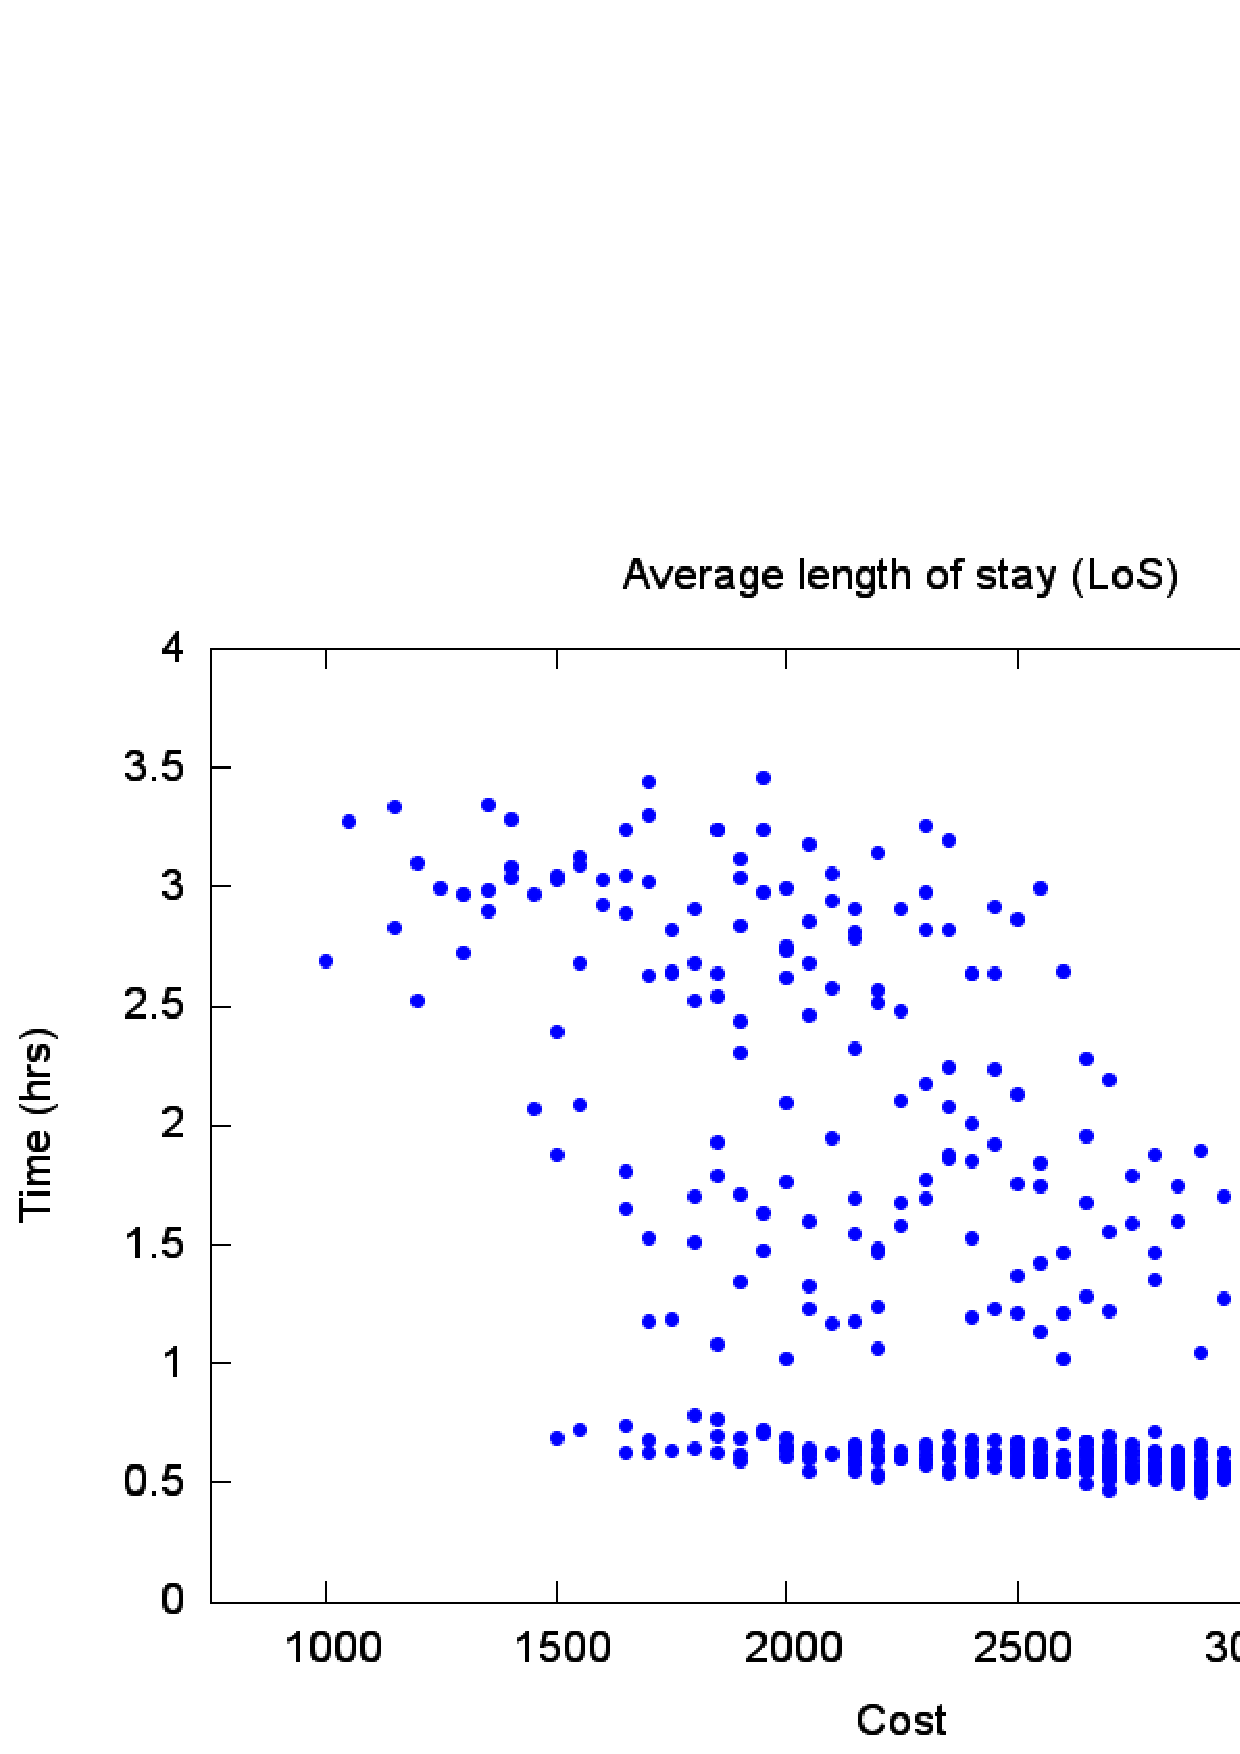
\includegraphics[width=0.95\columnwidth,height=0.23\paperheight]{figs4/v0/6400-602-25-exh-LoS-min}
\par\end{centering}

\caption{Average LoS obtained by the ES. The red triangle was the minimum.
\label{subfig:es4-1}}
\end{figure}


The PA result is shown in \ref{subfig:pipe4-1}, where four regions
can be clearly seen and the red triangle was the minimum. 
\begin{figure}[H]
\noindent \begin{centering}
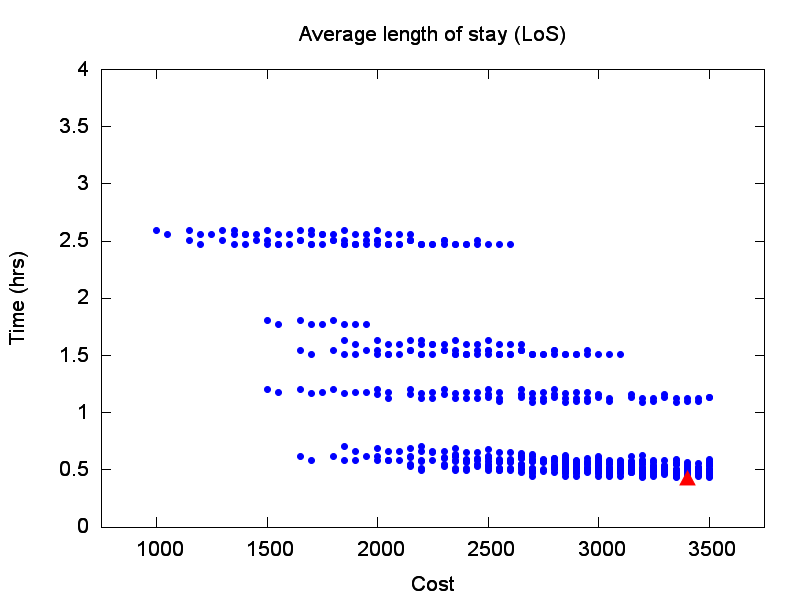
\includegraphics[width=0.95\columnwidth,height=0.23\paperheight]{figs4/v0/6400-602-25-pipe-LoS-min}
\par\end{centering}

\caption{Average LoS obtained by the PA. The red triangle was the minimum.
\label{subfig:pipe4-1}}
\end{figure}
The most important is the bottom region, in which the average minimum
LoS was around 0.5 hours. There were 366 configurations (from a total
of 602 in the feasible region) in this region, which is the one where
the minimum was.

The MC plus the K-means methods results are shown in \ref{subfig:mc4-1}
to \ref{subfig:km4-1}, respectively. The MC method found 75 configurations.
\begin{figure}[H]
\noindent \centering{}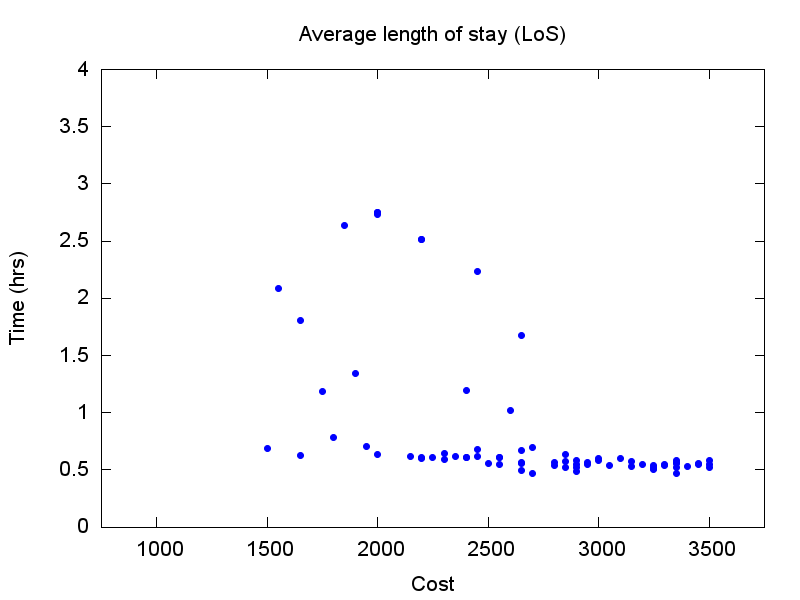
\includegraphics[width=0.95\columnwidth,height=0.23\paperheight]{figs4/v0/MC/MC-6400-602-25-69-25-75confs-LoS}\caption{Average LoS of 75 configurations obtained by the MC method. \label{subfig:mc4-1}}
\end{figure}
 However, it was difficult to get any conclusion about such region;
therefore, the complementary K-means method was performed. The K-means
method identified three different clusters, shown in \ref{subfig:km4-1}.
The most important cluster was the red one (at the bottom right),
which delimited the region where the optimum was. 
\begin{figure}[H]
\noindent \centering{}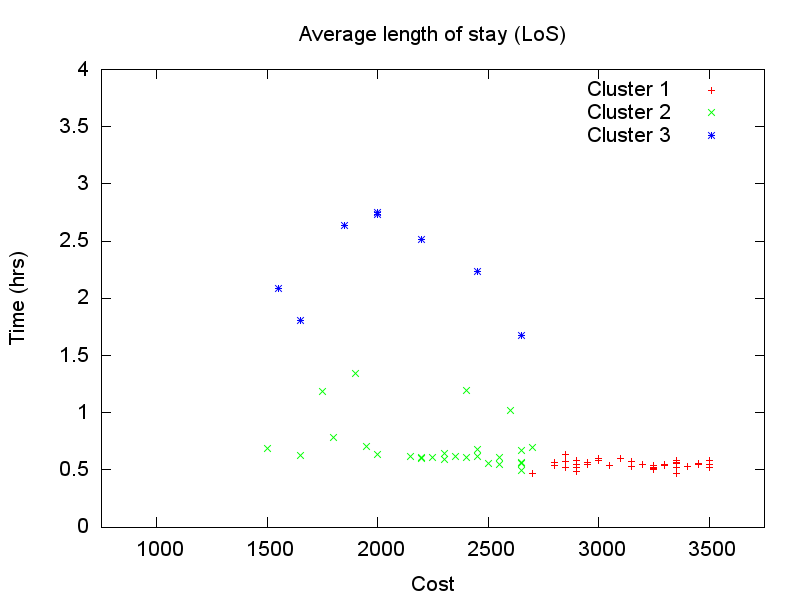
\includegraphics[width=0.95\columnwidth,height=0.23\paperheight]{figs4/v0/MC/K-means-6400-602-25-69-25-75-Cluster1-36_Cluster2-27_Cluster3-8}\caption{K-means identified three clusters of average LoS . The red one delimits
the region where the minimum was.\label{subfig:km4-1}}
\end{figure}
 %
\begin{comment}
but the green cluster was also important, because the average LoS
of such configurations were not so different from the red cluster.
\end{comment}


The \ref{fig:3D-scattered-graph-25} shows another way to visualise
the connectivity characteristic of the reduced regions found by the
proposed methodology. The axes of such graph are the equivalent operational
patient-service time \foreignlanguage{american}{(t{*})} of a ``single
one'' sanitary professional of each sanitary staff configuration
(the first column of \ref{subtab:As-pipe} to \ref{subtab:Ds-pipe},
where they were ordered by the PA \ref{eq:Pipeline formula}). In
such figure, the points of interest were the green points, which lie
in the region of interest, where the minimum was, which can be seen
in black triangle. It can be seen that it was not necessary to search
in the whole feasible region, but only in the green connected region. 

\begin{figure}[h]
\noindent \begin{centering}
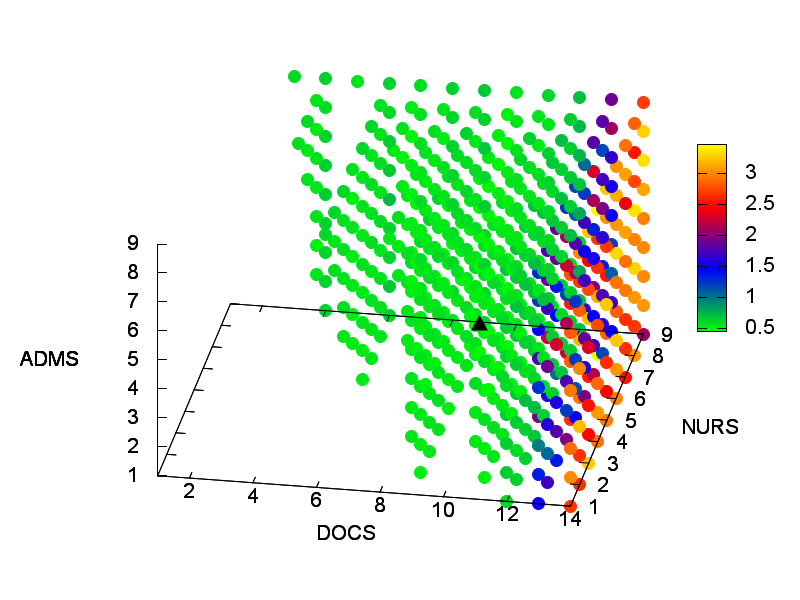
\includegraphics[width=0.95\columnwidth,height=0.2\paperheight]{figs4/v0/6400-602-25-3D-scatter-LoS2}
\par\end{centering}

\caption{3D scattered graph shows the average LoS index of the first workload
scenario (4 patients/hour). The average LoS index in hours is represented
in colour, and the minimum is the black triangle.\label{fig:3D-scattered-graph-25} }
\end{figure}


Finally, after separately applied both the PA and the MC plus the
K-means methods, the \textquotedblleft{}reduced exhaustive search\textquotedblright{}
was separately performed in each reduced region identified. The optimum
found per each method: the ES, the PA, and the MC plus the K-means
methods are presented in \ref{tab:4p-a}, where the sanitary staff
configuration (doctors, nurses, and admission personnel), their associated
average minimum LoS, and cost configuration are shown. The three optima
independently found were the same. 

\begin{comment}
\begin{figure}[H]
\noindent \begin{centering}
\begin{minipage}[t][1\totalheight][s]{0.95\columnwidth}%
\noindent \begin{center}
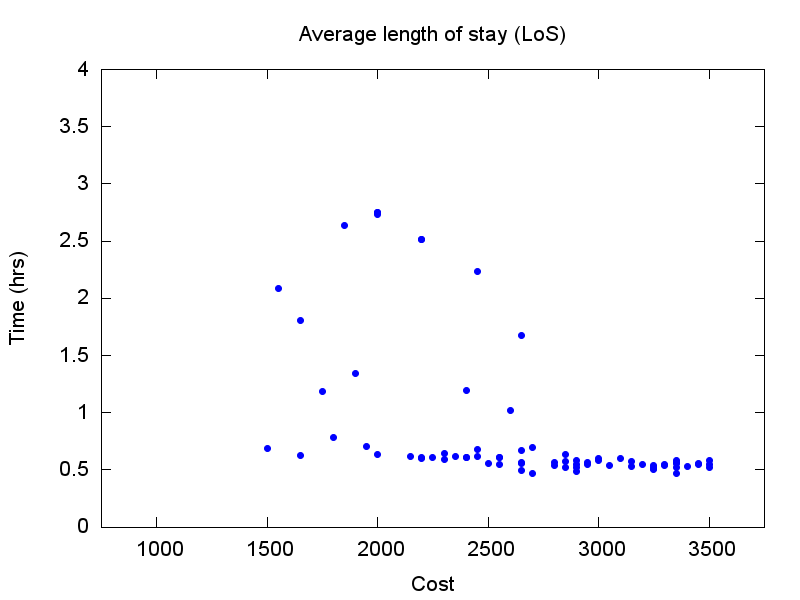
\includegraphics[width=0.95\columnwidth,height=0.25\paperheight]{figs4/v0/MC/MC-6400-602-25-69-25-75confs-LoS.png}
\par\end{center}

\vspace*{-1cm}

\noindent \begin{center}
\caption{Average LoS of 75 configurations obtained by the MC method. }

\par\end{center}%
\end{minipage}
\par\end{centering}

\noindent \begin{centering}
\vspace{0cm}
\vspace*{-1.2cm}
\par\end{centering}

\noindent \begin{centering}
\begin{minipage}[t][1\totalheight][s]{0.95\columnwidth}%
\noindent \begin{center}
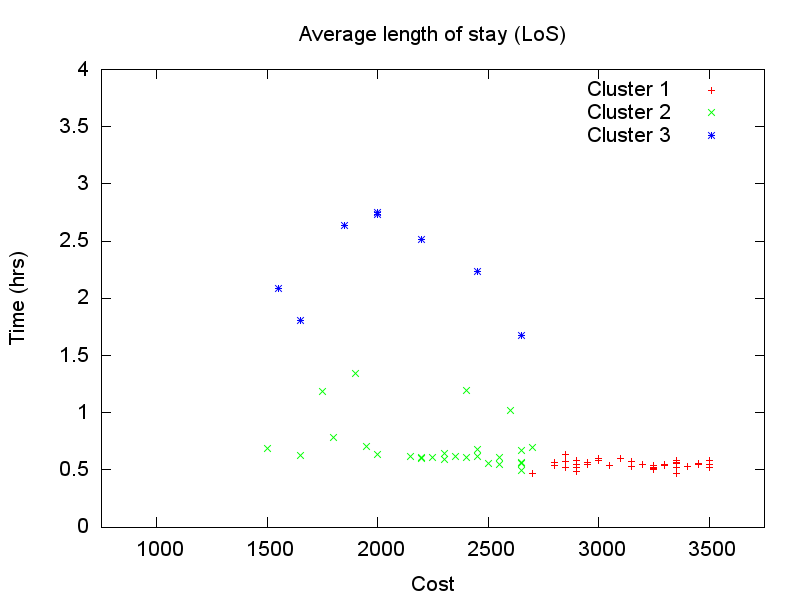
\includegraphics[width=0.95\columnwidth,height=0.25\paperheight]{figs4/v0/MC/K-means-6400-602-25-69-25-75-Cluster1-36_Cluster2-27_Cluster3-8.png}\vspace*{-0.8cm}
\par\end{center}

\caption{K-means identified three clusters of average LoS . The red one delimits
the region where the minimum is.}
%
\end{minipage}
\par\end{centering}

%\vspace*{0.4cm}%{\bf Figures} show the average LoS index of the first workload scenario (4 patients/hour) using the ES, the PA, and the MC+K-means methods.
\end{figure}
\end{comment}
%\vspace*{-.2cm}%
\begin{comment}
 \begin{figure}[htb!]  
\centering 
\begin{tabular}{cc}         
	\subfloat[][Average patient LOS with P = 20\%]{                 		\includegraphics[width=75mm,height=60mm]{figs4/v0/6400-602-25-pacs-totales-sort-pipe-meantime-exh-min-CINCO.pdf} 
		\label{subfloat:exp1_20} 
	} 
&        
	\subfloat[][Average patient LOS with P = 40\%]{                 		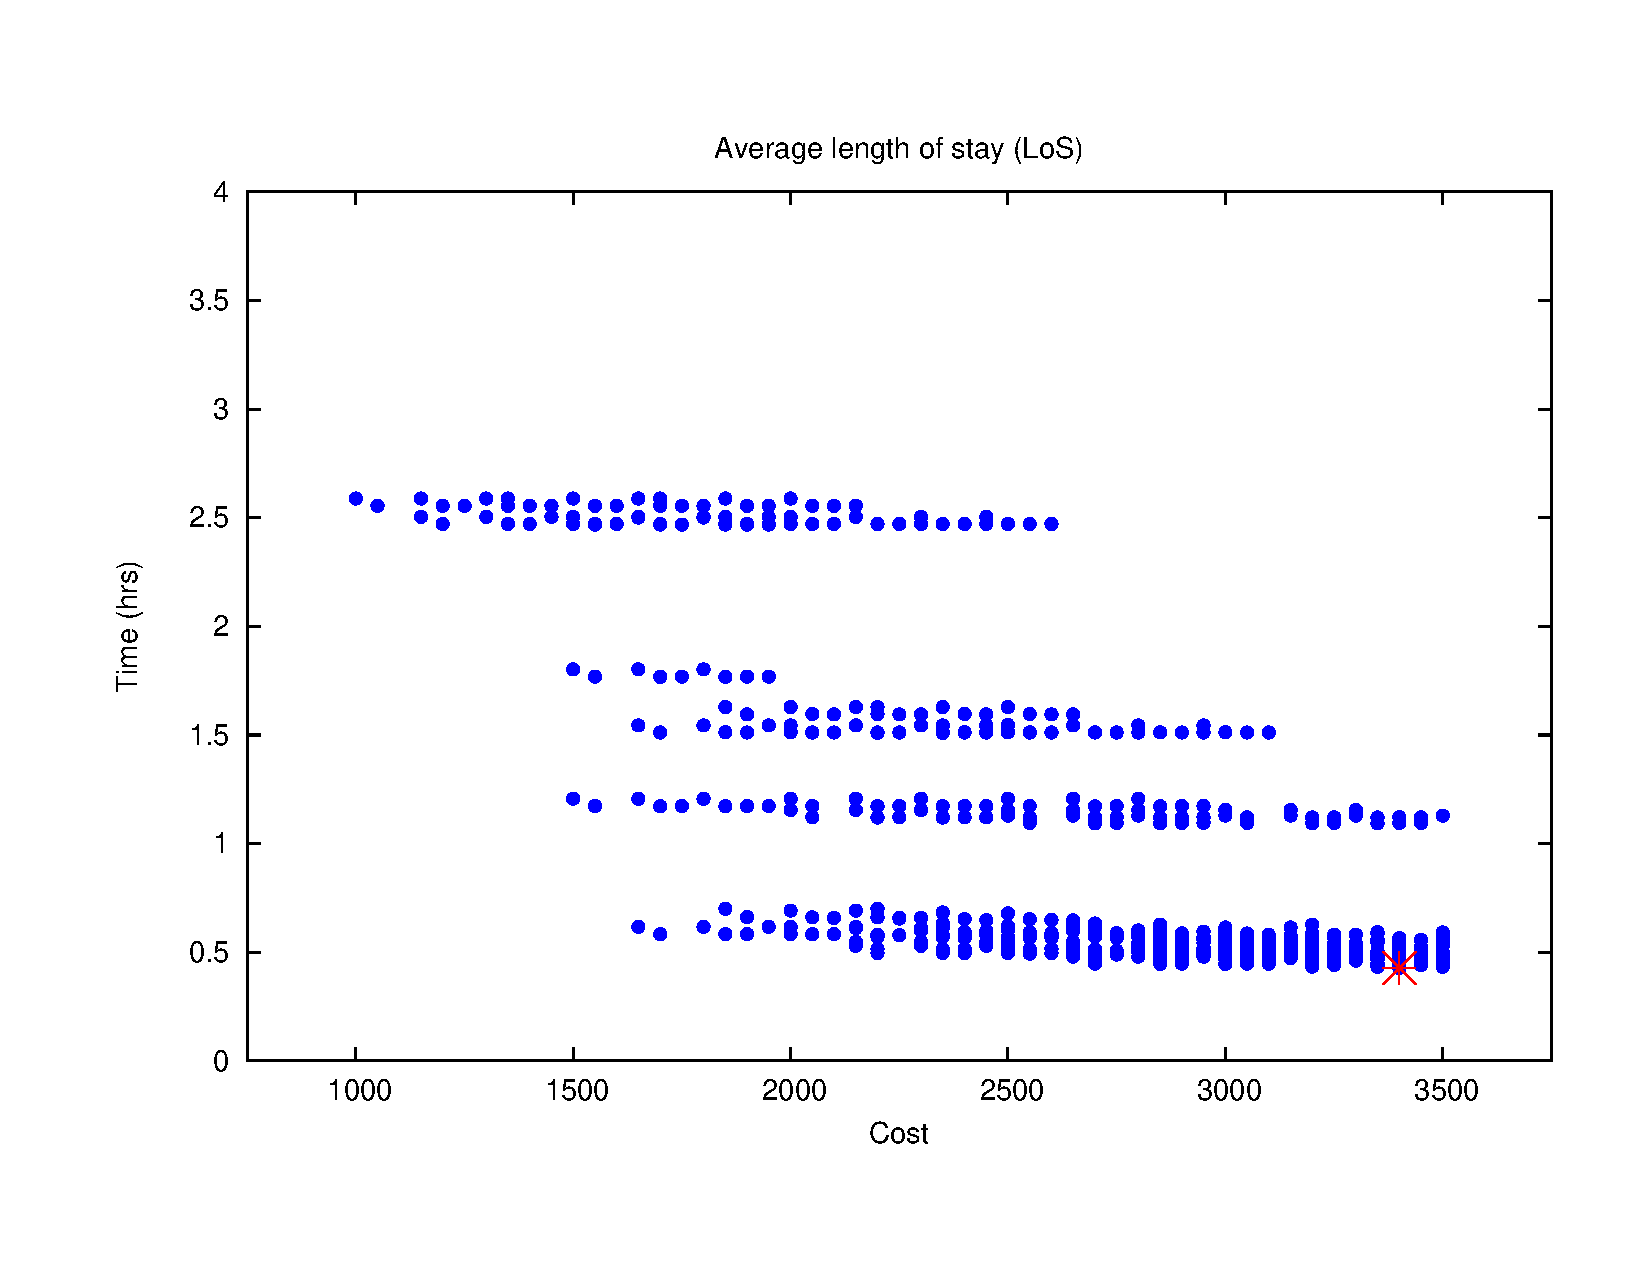
\includegraphics[width=75mm,height=60mm]{figs4/v0/pipe-sorted-LoS_0-25_min.pdf}                 		\label{subfloat:exp1_40}        
} 
\\ 	
	\subfloat[][Average patient LOS with P = 20\%]{                 		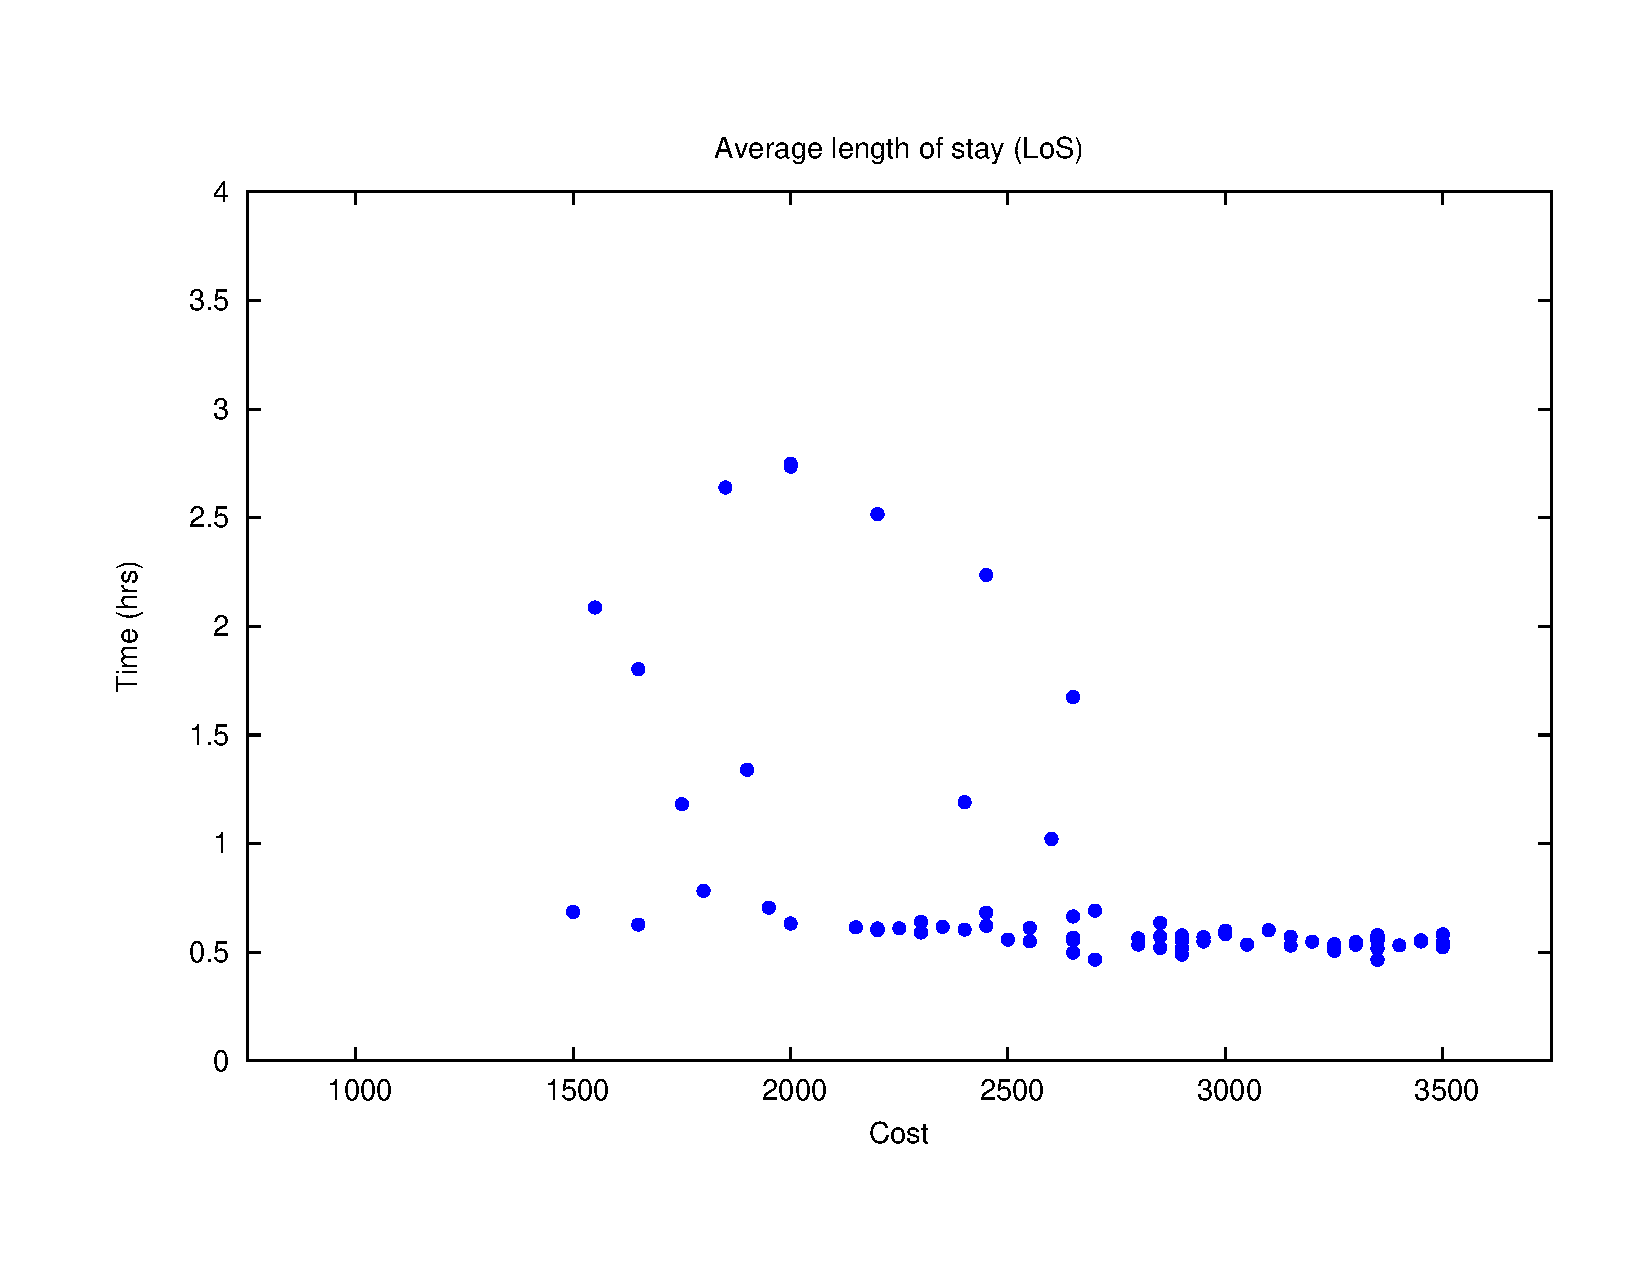
\includegraphics[width=75mm,height=60mm]{figs4/v0/MC/MC-6400-602-25-69-25-75confs-LoS-TRI.pdf} 
		\label{subfloat:exp1_20} 
	} 
& 
 \subfloat[][Average patient LOS with P = 40\%]{                 		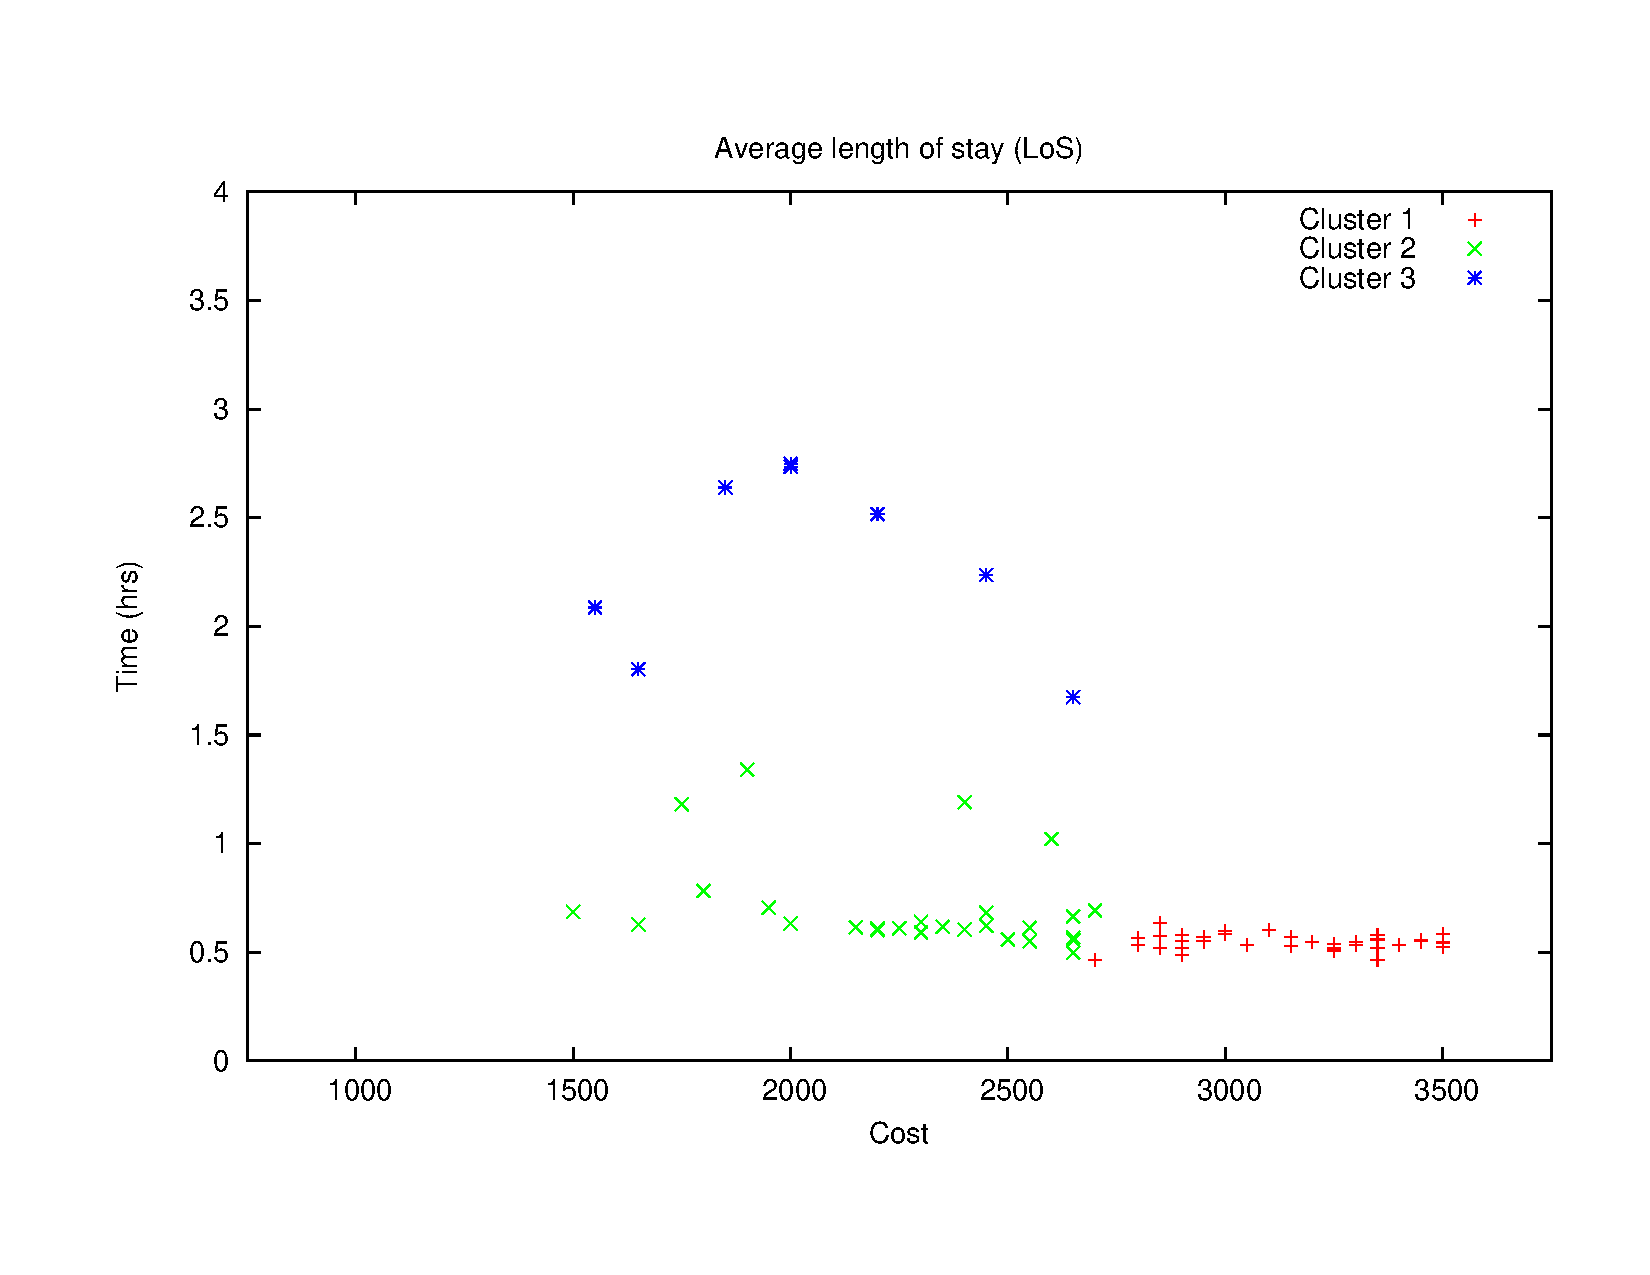
\includegraphics[width=75mm,height=60mm]{figs4/v0/MC/K-means-6400-602-25-69-25-75-Cluster1-36_Cluster2-27_Cluster3-8_TRI.pdf}                 		
		\label{subfloat:exp1_40}        
} 
\end{tabular}
\caption{Average patient LOS. Red and green points are the minimum.} 
\label{fig:exp1_20_40} 
\end{figure} 
\end{comment}
\begin{comment}
\begin{figure}[H]
\noindent \begin{centering}
\begin{minipage}[t][1\totalheight][s]{0.49\columnwidth}%
\noindent \begin{center}
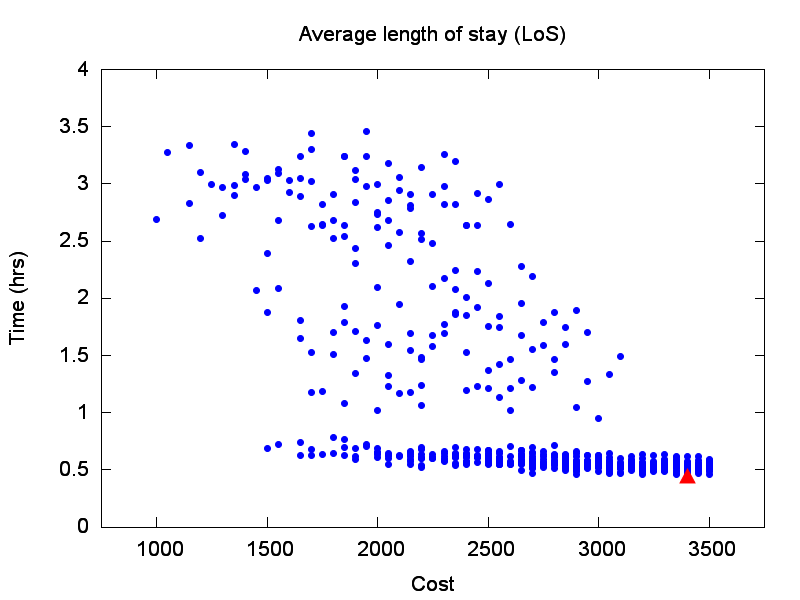
\includegraphics[width=1\columnwidth]{figs4/v0/6400-602-25-exh-LoS-min.png}
\par\end{center}

\vspace*{-1cm}

\noindent \begin{center}
\caption{Average LoS obtained by the ES method. The red triangle was the minimum.
\label{subfig:es4}}

\par\end{center}%
\end{minipage}\hfill{}%
\begin{minipage}[t][1\totalheight][s]{0.49\columnwidth}%
\noindent \begin{center}
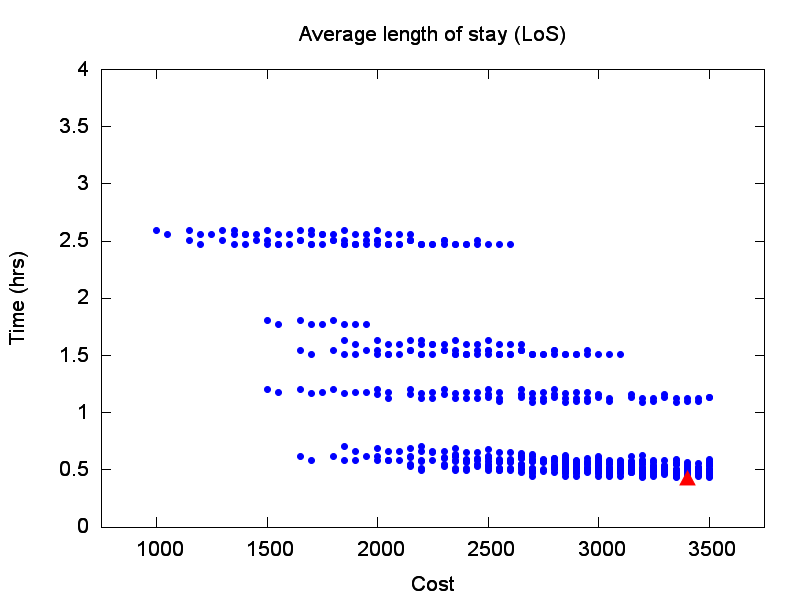
\includegraphics[width=1\columnwidth]{figs4/v0/6400-602-25-pipe-LoS-min.png}
\par\end{center}

\vspace*{-1cm}

\noindent \begin{center}
\caption{Average LoS obtained by the PA. The red triangle is the minimum. \label{subfig:pipe4}}

\par\end{center}%
\end{minipage}
\par\end{centering}

\noindent \begin{centering}
%\centering\vspace{0cm}
\vspace*{-1.2cm}
\par\end{centering}

\begin{minipage}[t][1\totalheight][s]{0.49\columnwidth}%
\noindent \begin{center}
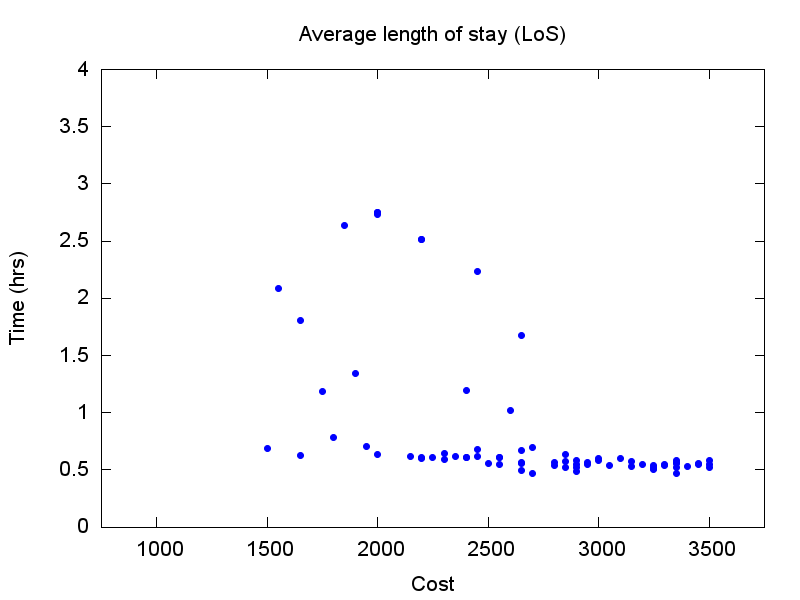
\includegraphics[width=1\columnwidth]{figs4/v0/MC/MC-6400-602-25-69-25-75confs-LoS.png}\vspace*{-0.8cm}
\par\end{center}

\caption{Average LoS of 75 configurations obtained by the MC method. \label{subfig:mc4}}
%
\end{minipage}\hfill{}%
\begin{minipage}[t][1\totalheight][s]{0.49\columnwidth}%
\noindent \begin{center}
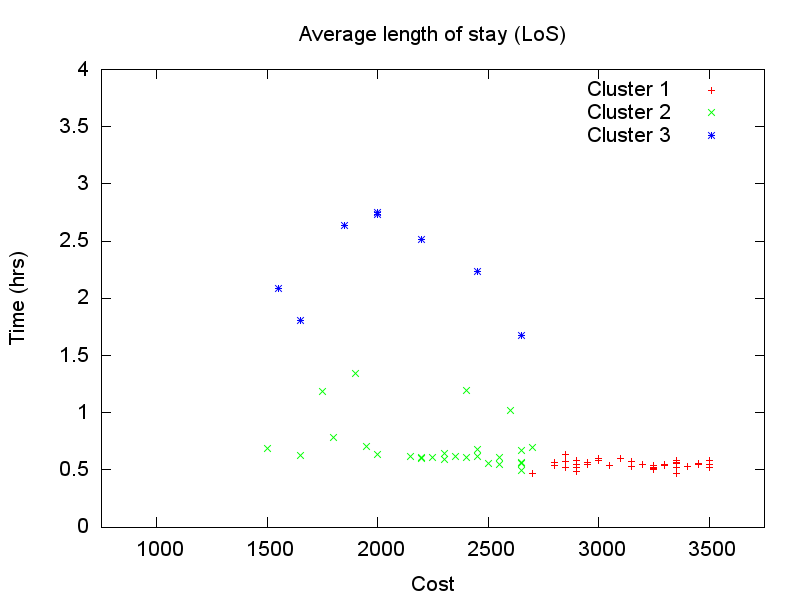
\includegraphics[width=1\columnwidth]{figs4/v0/MC/K-means-6400-602-25-69-25-75-Cluster1-36_Cluster2-27_Cluster3-8.png}\vspace*{-0.8cm}
\par\end{center}

\caption{The K-means method identified three clusters of average LoS. The red
one delimited the region where the minimum was.\label{subfig:km4}}
%
\end{minipage}

\vspace*{0.4cm}{\bf Figures} show the average LoS index of the first workload scenario (4 patients/hour) using the ES, the PA, and the MC+K-means methods.
\end{figure}
\end{comment}
\begin{comment}
\begin{figure}[H]
\hfill{}\subfloat[\label{subfloat:pipe4} Scattered 3D graph of doctors, nurses, and
admission personnel.]{

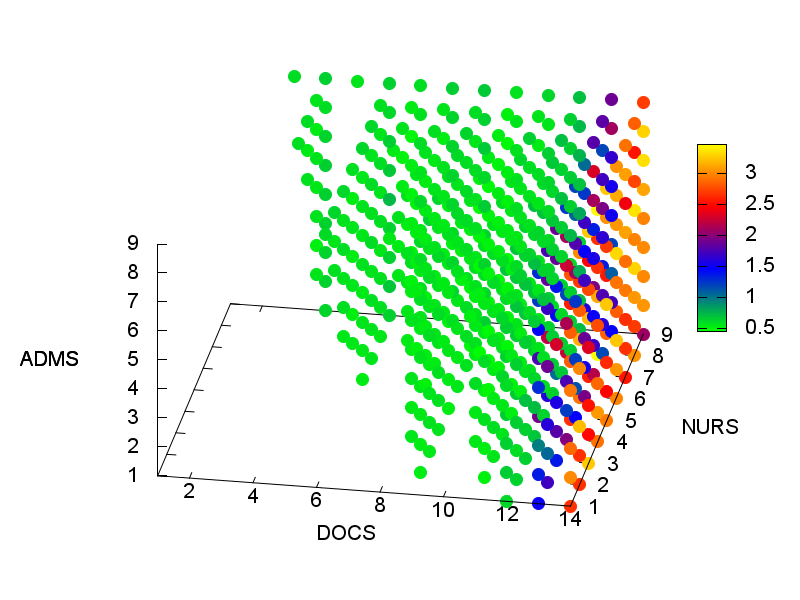
\includegraphics[width=0.48\columnwidth]{figs4/6400-602-25-3D-scatter-LoS.png}}\hfill{}\subfloat[\label{subfloat:contour4} Contour graph where doctors and nurses
can be seen.]{

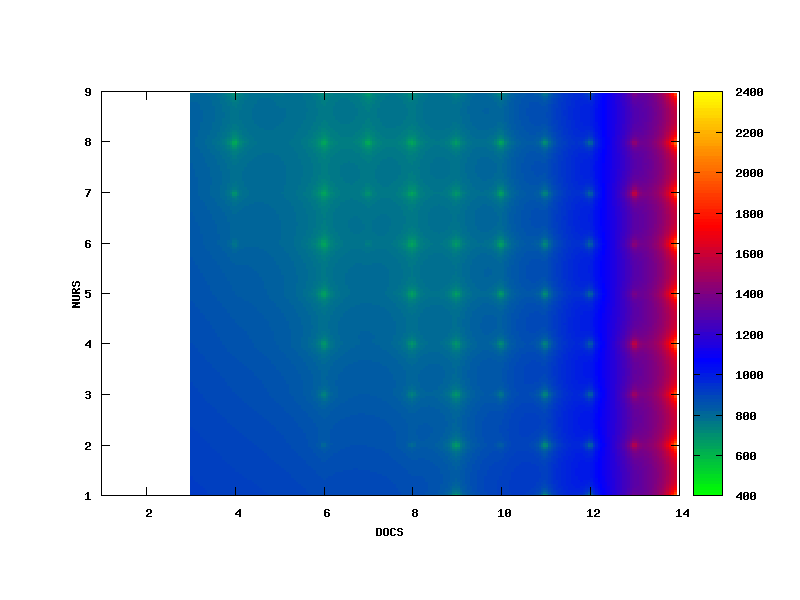
\includegraphics[width=0.48\columnwidth]{figs4/6400-602-25-sort-pipe_p5_y_p4-contour.png}}\hfill{}

\caption{\label{fig:Two-vision} Graphs show the average LoS index of the first
workload scenario (4 patients/hour) using the first column of \ref{subtab:As-pipe},
\ref{subtab:Ns-pipe}, and \ref{subtab:Ds-pipe}, where they were
ordered by the pipeline approach (PA) \ref{eq:Pipeline formula}.
The colour bar is expresed in tics ( $hours\:=\frac{tics}{1000}$
).}
\end{figure}
\end{comment}
\begin{comment}
\begin{figure}[H]
\noindent \begin{centering}
\begin{minipage}[t][1\totalheight][s]{1\columnwidth}%
 %
\noindent \begin{center}
\centering\foreignlanguage{british}{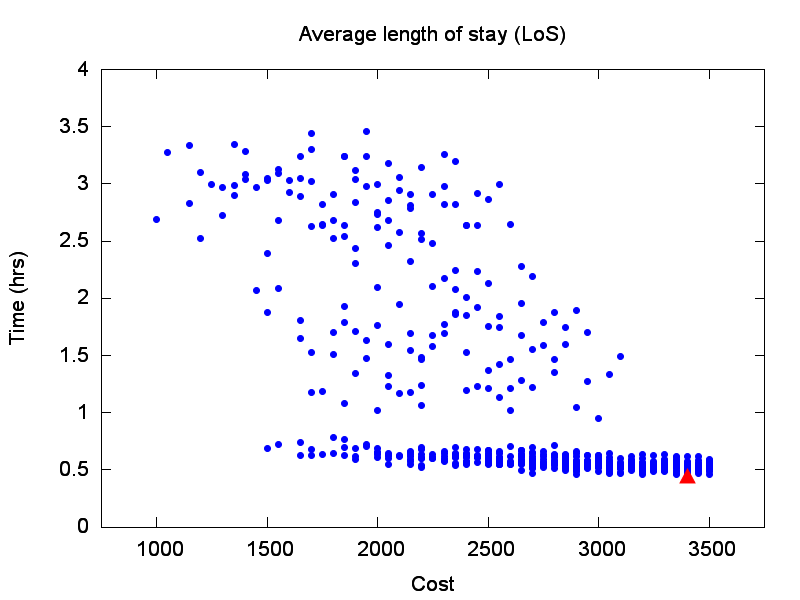
\includegraphics[scale=0.4]{figs4/v0/6400-602-25-exh-LoS-min.png}}
\par\end{center}

  %
\vspace*{-1cm}

\noindent \begin{center}
\caption{Average LoS obtained by the ES method, the red triangle is the minimum. }

\par\end{center}%
\end{minipage}
\par\end{centering}

\noindent \begin{centering}
%\centering\vspace{0cm}
\vspace*{-1.2cm}
\par\end{centering}

\noindent \begin{centering}
\begin{minipage}[t][1\totalheight][s]{1\columnwidth}%
\noindent \begin{center}
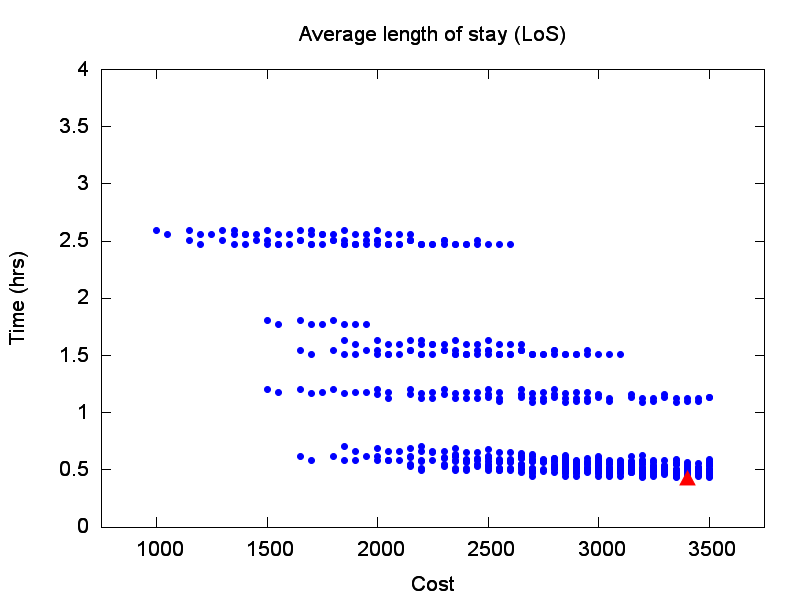
\includegraphics[scale=0.4]{figs4/v0/6400-602-25-pipe-LoS-min.png}\vspace*{-0.8cm}
\par\end{center}

\caption{Average LoS obtained by the PA, the red triangle is the minimum. }
%
\end{minipage}
\par\end{centering}

\noindent %\vspace*{0.4cm}%{\bf Figures} show the average LoS index of the first workload scenario (4 patients/hour) using the ES, the PA, and the MC+K-means methods.
\end{figure}
\end{comment}


\begin{table}[H]
\caption{Optimum staff configurations that got the average minimum LoS for
this workload scenario (up to 4 patients hourly), where S is Senior
and J is Junior. This optimum sanitary staff configuration is shown
in red triangle in \ref{subfig:es4-1} and in black triangle in \ref{fig:3D-scattered-graph-25}.}


\centering{}%
\begin{tabular}{cccccc>{\centering}p{2.8cm}}
\hline 
Method & � & LoS (hrs) & D & N & A & Run time (hrs)

4 Pthreads\tabularnewline
\hline 
ES & 3,400  & 0.44 & 2S  & 2S & 2S & 0.89\tabularnewline
PA & 3,400 & 0.43 & 2S & 2S & 2S & 0.53\tabularnewline
MC+K-means & 3,400  & 0.44 & 2S  & 2S & 2S & 0.76\tabularnewline
\hline 
\end{tabular}\label{tab:4p-a} 
\end{table}


\begin{comment}
From Figures \ref{fig:exp1_20} and \ref{tab:4p-a}, there is a staff
configuration that got the minimum time. Also, in such Figures \ref{fig:exp1_20}
can appreciate that there are many other staff configurations that
are quite close to the optimum, but with less cost.
\end{comment}



\subsubsection{Second Workload Scenario}

The results of this scenario, up to 9 patients/hour, are shown from
\ref{subfig:es8-1} to \ref{subfig:km8-1}. The ES result is shown
in \ref{subfig:es8-1}, where the red triangle was the minimum. 
\begin{figure}[H]
\noindent \begin{centering}
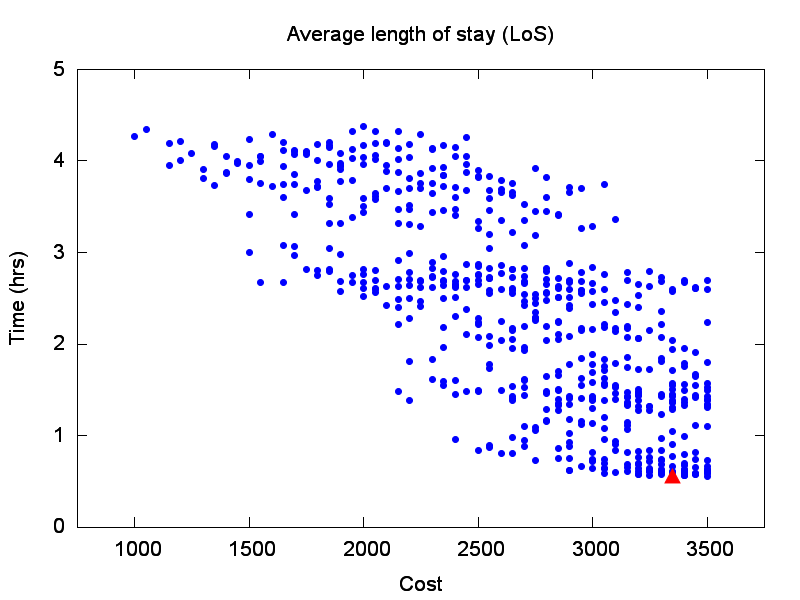
\includegraphics[width=0.95\columnwidth,height=0.25\paperheight]{figs4/v0/6400-602-50-exh-LoS-min}
\par\end{centering}

\caption{Average LoS obtained by the ES. The red triangle was the minimum.
\label{subfig:es8-1}}
\end{figure}


The PA result is shown in \ref{subfig:pipe8-1}, where seven regions
can be clearly seen and the red triangle is the minimum.
\begin{figure}[H]
\noindent \begin{centering}
\includegraphics[width=0.95\columnwidth,height=0.25\paperheight]{figs4/v0/pipe-sorted-LoS_0\lyxdot 50_min}
\par\end{centering}

\caption{Average LoS obtained by the PA. The red triangle was the minimum.
\label{subfig:pipe8-1}}
\end{figure}
 The most important is the bottom region, in which the average minimum
LoS was around 1 hour. There were 180 configurations (from a total
of 602 in the feasible region) in this region, which is the one where
the minimum was.

The MC plus the K-means methods results are shown in \ref{subfig:mc8-1}
to \ref{subfig:km8-1}, respectively. The MC method found 125 configurations.
\begin{figure}[H]
\noindent \centering{}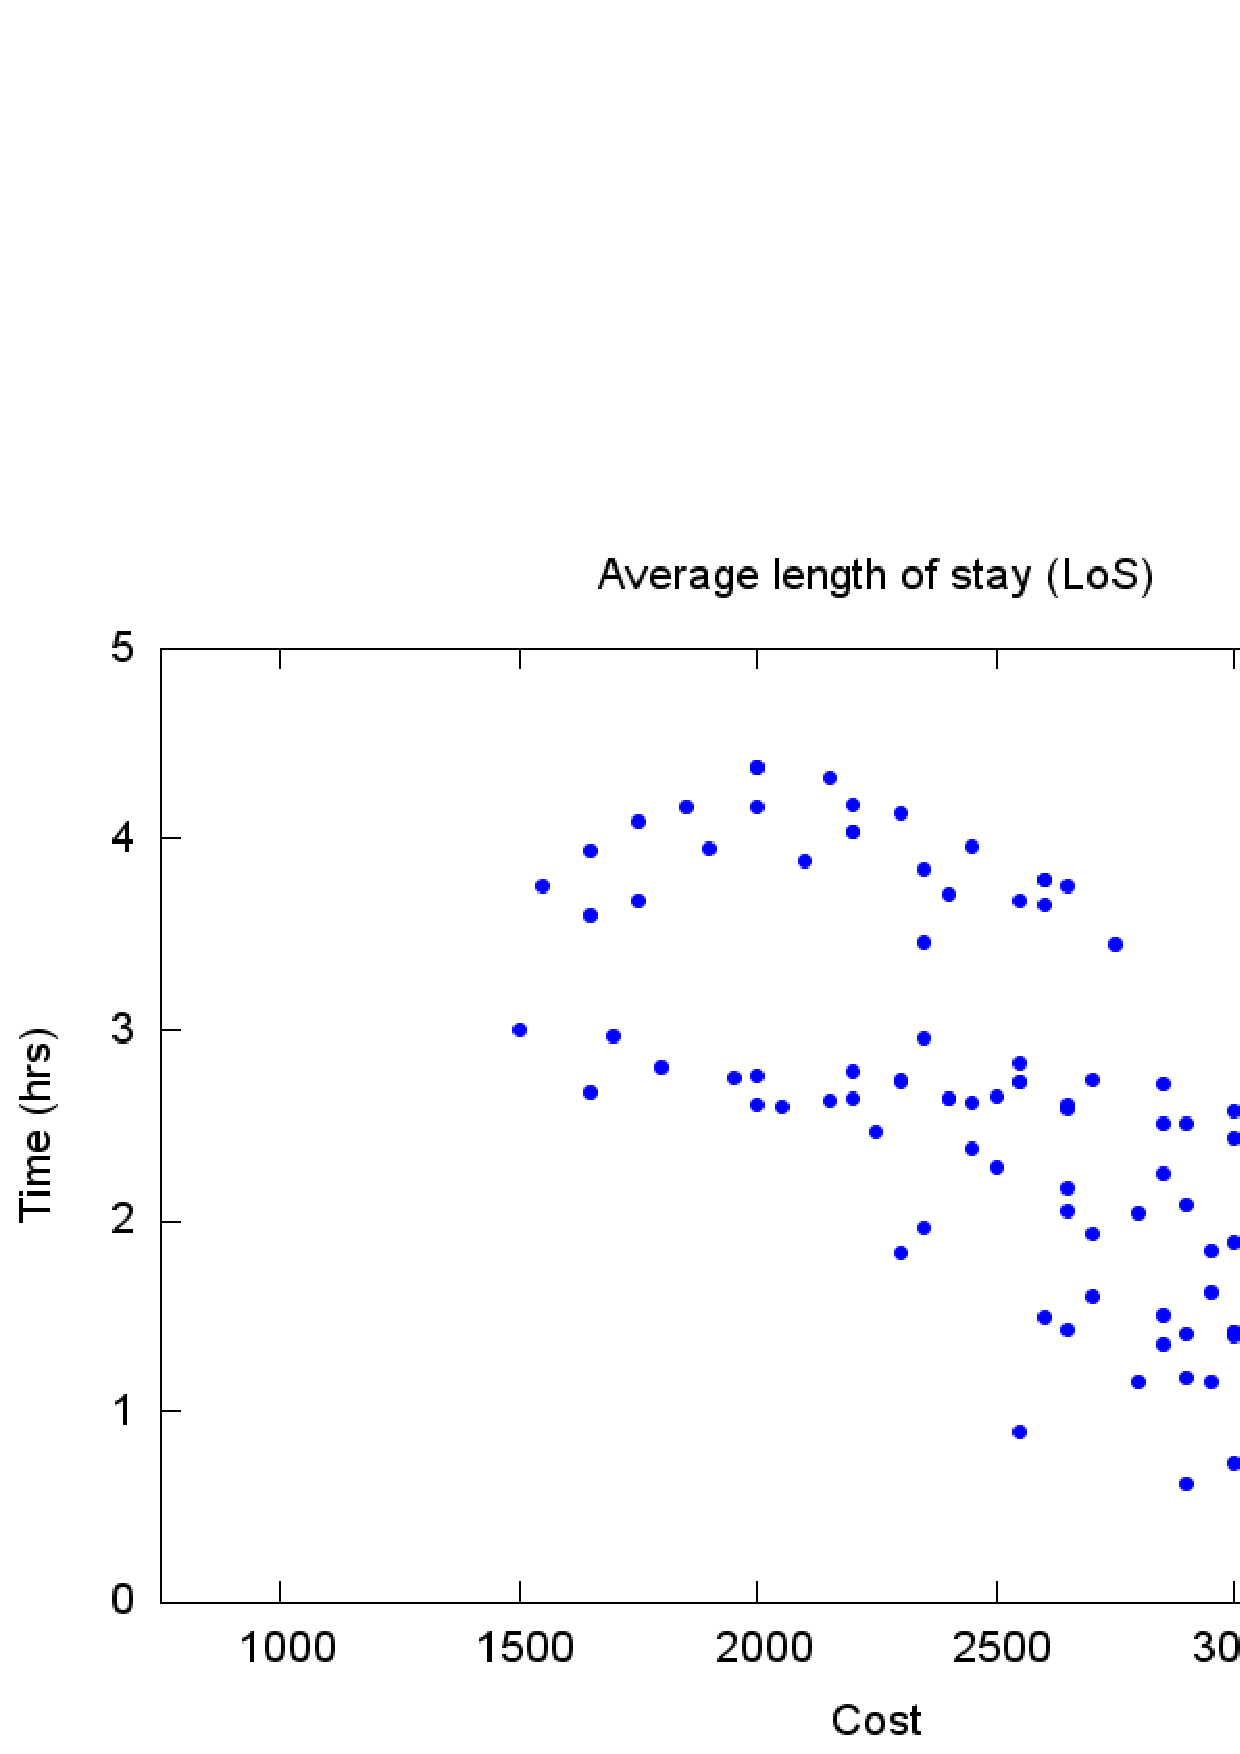
\includegraphics[width=0.95\columnwidth,height=0.25\paperheight]{figs4/v0/MC/MC-6400-602-50-69-25-125confs-LoS}\caption{Average LoS of 125 configurations obtained by the MC method. \label{subfig:mc8-1}}
\end{figure}
However, it was difficult to get any conclusion about such region;
therefore, the complementary K-means method was performed. The K-means
method identified two different clusters, shown in \ref{subfig:km8-1}.
The most important was the green cluster (at the bottom right), which
delimited the region where the optimum was.
\begin{figure}[H]
\noindent \centering{}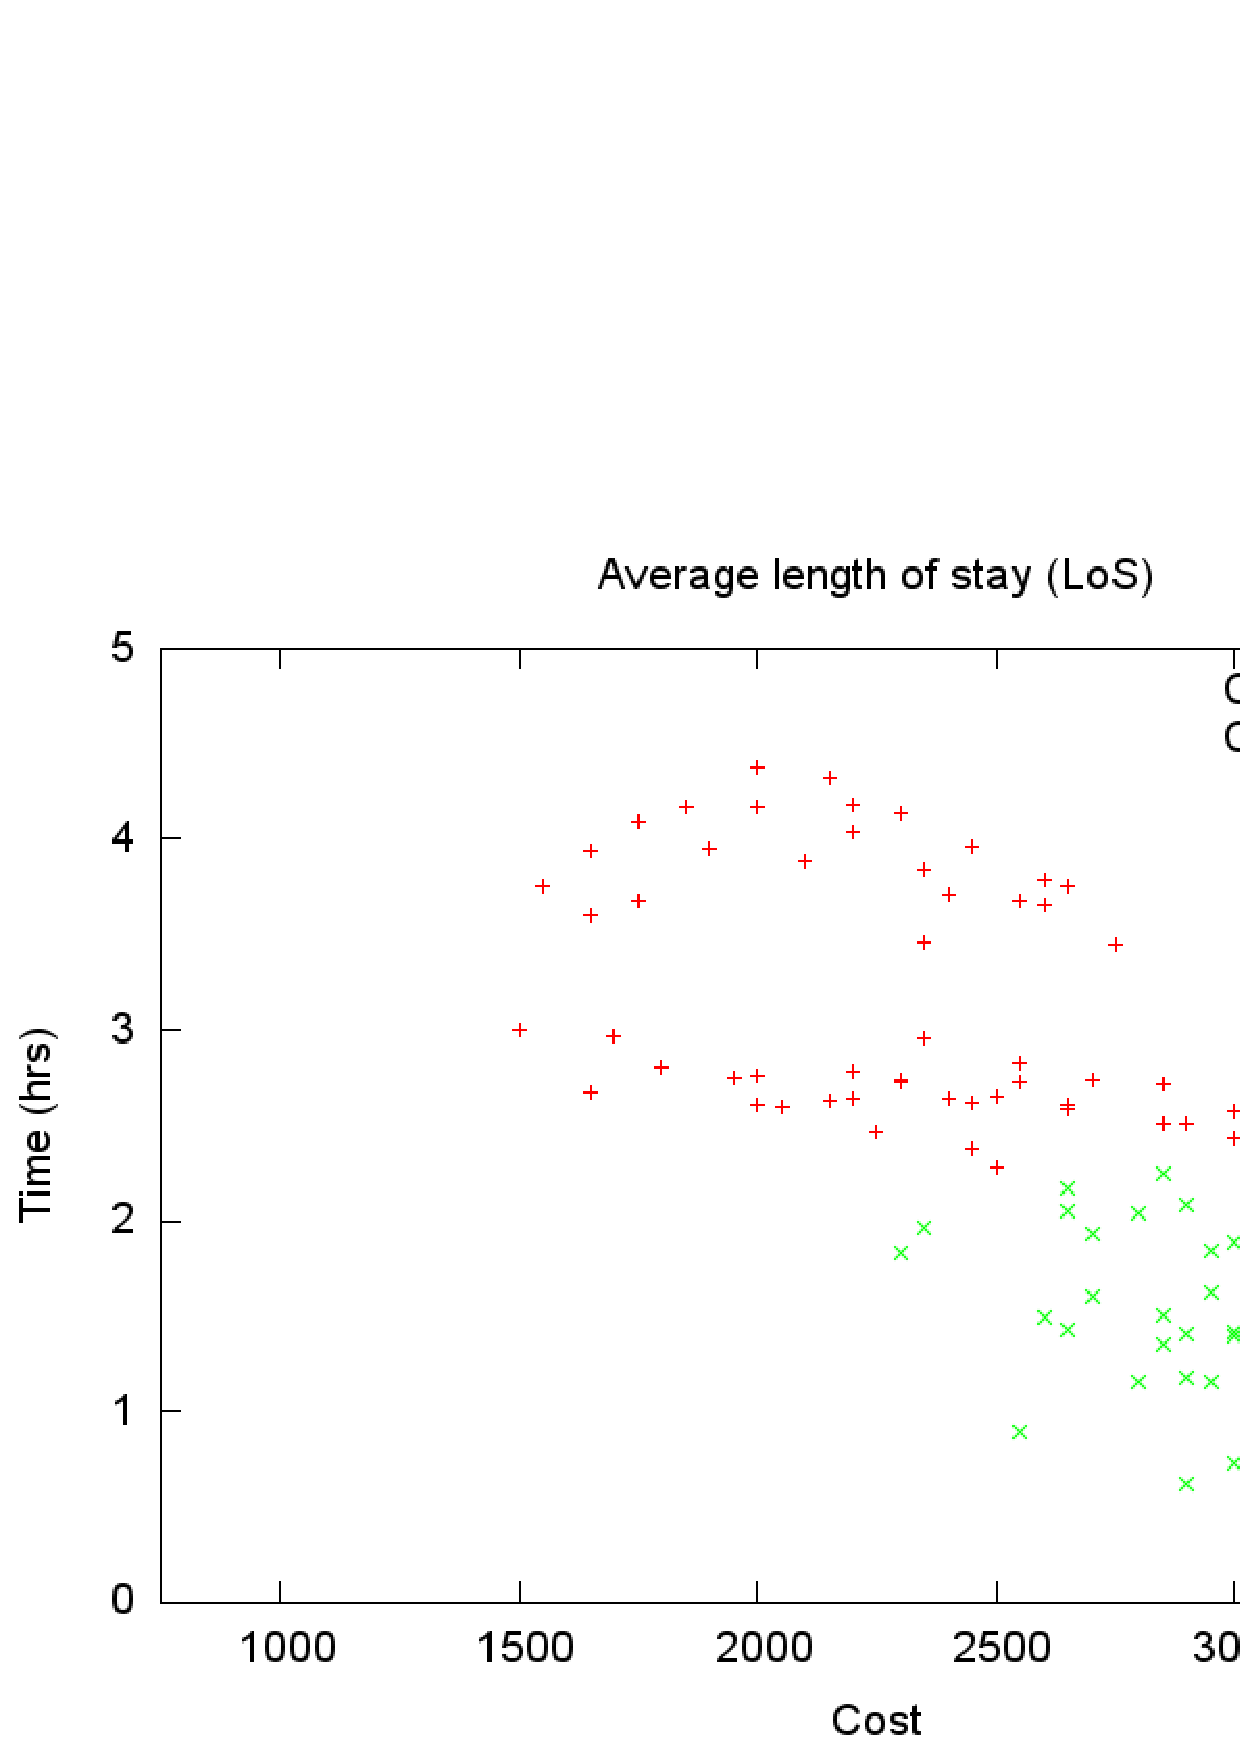
\includegraphics[width=0.95\columnwidth,height=0.25\paperheight]{figs4/v0/MC/K-means-6400-602-50-69-25-125-Cluster1-58_Cluster2-58}\caption{The K-means method identified two clusters of average LoS. The green
one delimited the region where the minimum was.\label{subfig:km8-1}}
\end{figure}


The \ref{fig:3D-scattered-graph-50} shows another way to visualise
the connectivity characteristic of the reduced regions found by the
proposed methodology. The axes of such graph are the equivalent operational
patient-service time \foreignlanguage{american}{(t{*})} of a ``single
one'' sanitary professional of each sanitary staff configuration
(the first column of \ref{subtab:As-pipe} to \ref{subtab:Ds-pipe},
where they were ordered by the PA \ref{eq:Pipeline formula}). In
such figure, the points of interest were the green points, which lie
in the region of interest, where the minimum was, which can be seen
in black triangle. It can be seen that it was not necessary to search
in the whole feasible region, but only in the green connected region.
\begin{figure}[H]
\noindent \begin{centering}
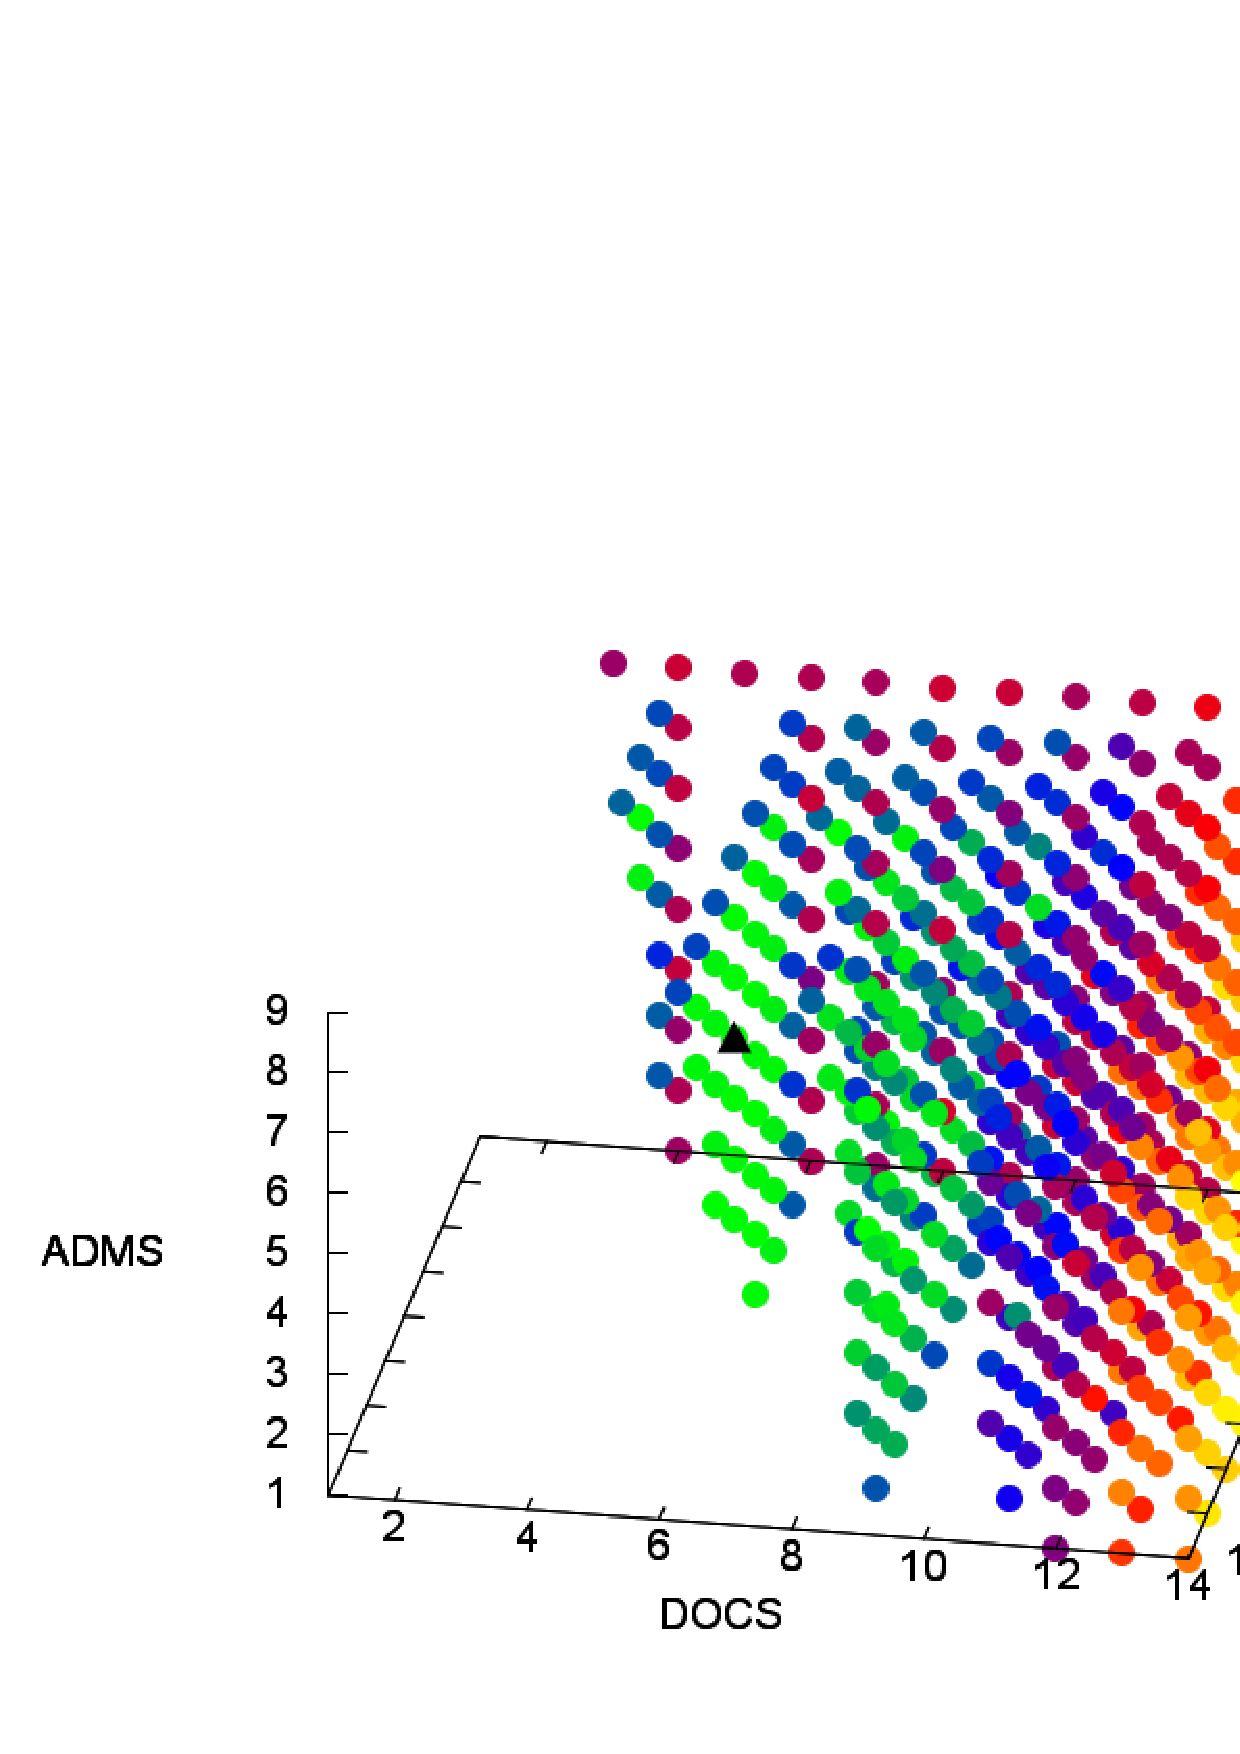
\includegraphics[width=0.95\columnwidth,height=0.2\paperheight]{figs4/v0/6400-602-50-3D-scatter-LoS2}
\par\end{centering}

\caption{3D scattered graph shows the average LoS index of the third workload
scenario (9 patients/hour). The average LoS index is expressed in
colour in hours.\label{fig:3D-scattered-graph-50}}
\end{figure}


Finally, after separately applied both the PA and the MC plus the
K-means methods, the \textquotedblleft{}reduced exhaustive search\textquotedblright{}
was separately performed in each reduced region identified. The optimum
found per each method: the ES, the PA, and the MC plus the K-means
methods are presented in \ref{tab:8p-a}, where the sanitary staff
configuration (doctors, nurses, and admission personnel), their associated
average minimum LoS, and cost configuration are shown. The three optima
 independently found were the same. 

\begin{comment}
Each staff configuration that got the minimum is presented in \ref{tab:4p-a},
\ref{tab:8p-a}, \ref{tab:12p-a}, and \ref{tab:16p-a}.
\end{comment}
\begin{comment}
\begin{figure}[h]
\hfill{}\subfloat[\label{subfloat:pipe8}Scattered 3D graph of doctors, nurses, and
admission personnel.]{

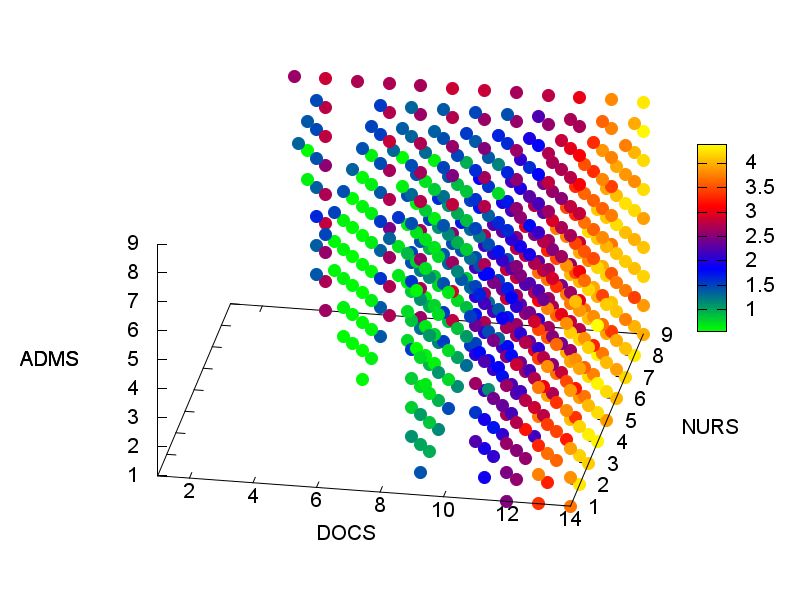
\includegraphics[width=0.48\columnwidth]{figs4/6400-602-50-3D-scatter-LoS.png}}\hfill{}\subfloat[\label{subfloat:contour8} Contour graph where doctors and nurses
can be seen.]{

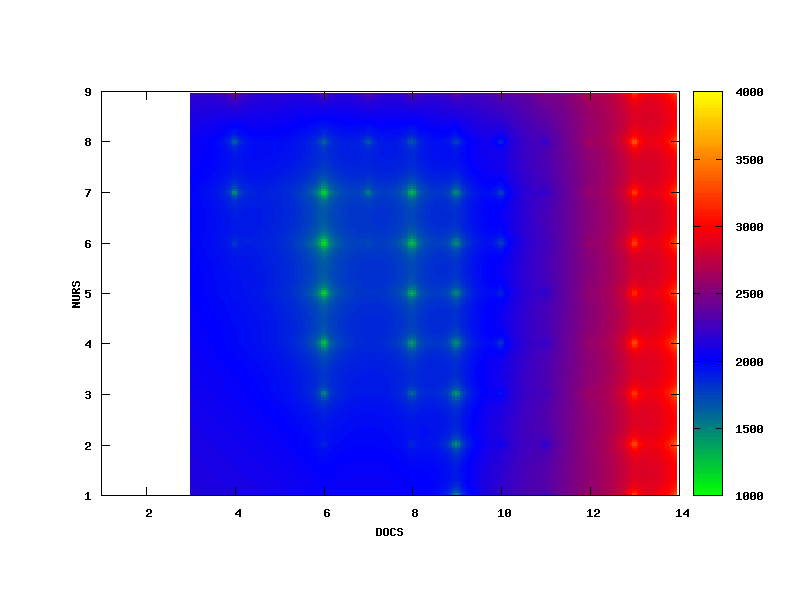
\includegraphics[width=0.48\columnwidth]{figs4/6400-602-50-sort-pipe_p5_y_p4-contour.png}}\hfill{}

\caption{\label{fig:Two-vision2} Graphs show the average LoS index of the
second workload scenario (9 patients/hour) using the first column
of \ref{subtab:As-pipe}, \ref{subtab:Ns-pipe}, and \ref{subtab:Ds-pipe},
where they were ordered by the pipeline approach (PA) \ref{eq:Pipeline formula}.
The colour bar is expresed in tics ( $hours\:=\frac{tics}{1000}$
). }
\end{figure}
\end{comment}
\vspace*{-.2cm}

\begin{table}[H]
\caption{Optimum staff configurations that got the average minimum LoS for
this workload scenario (up to 9 patients hourly), where S is Senior
and J is Junior. This optimum sanitary staff configuration is shown
in red triangle in \ref{subfig:es8-1} and in black triangle in \ref{fig:3D-scattered-graph-50}.}


\centering{}%
\begin{tabular}{cccccc>{\centering}p{2.8cm}}
\hline 
Method & � & LoS (hrs) & D & N & A & Run time (hrs)

4 Pthreads\tabularnewline
\hline 
ES & 3,350  & 0.55 & 4J & 2S & 1S,1J & 1.57\tabularnewline
PA & 3,350  & 0.55 & 4J & 2S & 1S,1J & 0.39\tabularnewline
MC+K-means & 3,350  & 0.55 & 4J & 2S & 1S,1J & 1.01\tabularnewline
\hline 
\end{tabular}\label{tab:8p-a} 
\end{table}


\clearpage{}


\subsubsection{Third Workload Scenario}

The results of this scenario, up to 13 patients/hour, are shown from
\ref{subfig:es13-1} to \ref{subfig:km13-1}. The ES result is shown
in \ref{subfig:es13-1}, where the red triangle was the minimum.
\begin{figure}[H]
\noindent \begin{centering}
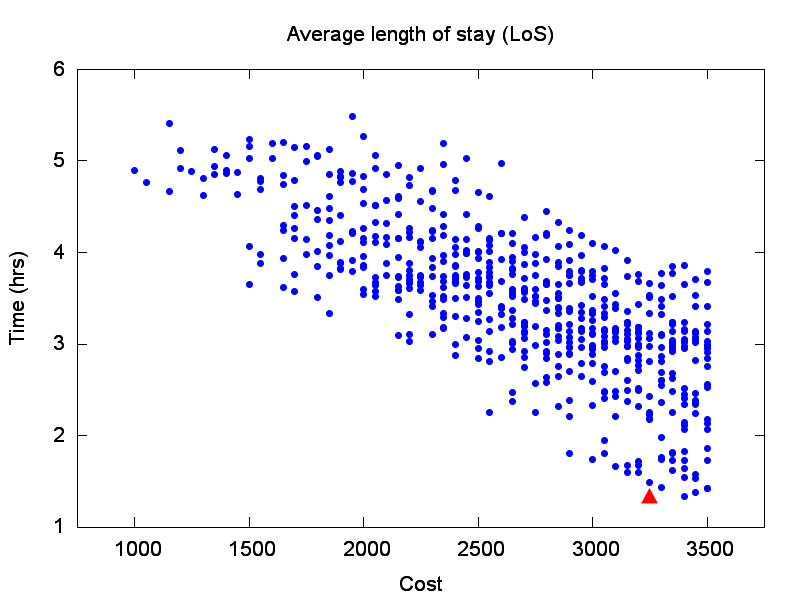
\includegraphics[width=0.95\columnwidth,height=0.25\paperheight]{figs4/v0/6400-602-75-exh-LoS-min}
\par\end{centering}

\caption{Average LoS obtained by the ES. The red triangle was the minimum.
\label{subfig:es13-1}}
\end{figure}


The PA result is shown in \ref{subfig:pipe13-1}, where many regions
can be clearly seen and the red triangle is the minimum. 
\begin{figure}[H]
\noindent \begin{centering}
\includegraphics[width=0.95\columnwidth,height=0.25\paperheight]{figs4/v0/pipe-sorted-LoS_0\lyxdot 75_min}
\par\end{centering}

\caption{Average LoS obtained by the PA. The red triangle was the minimum.
\label{subfig:pipe13-1}}
\end{figure}
 The most important is the bottom region, in which the average minimum
LoS was less than 2 hours. There were 21 configurations (from a total
of 602 in the feasible region) in this region, which is the one where
the minimum was.

The MC plus the K-means methods results are shown in \ref{subfig:mc13-1}
to \ref{subfig:km13-1}, respectively. The MC method found 125 configurations.
\begin{figure}[H]
\noindent \centering{}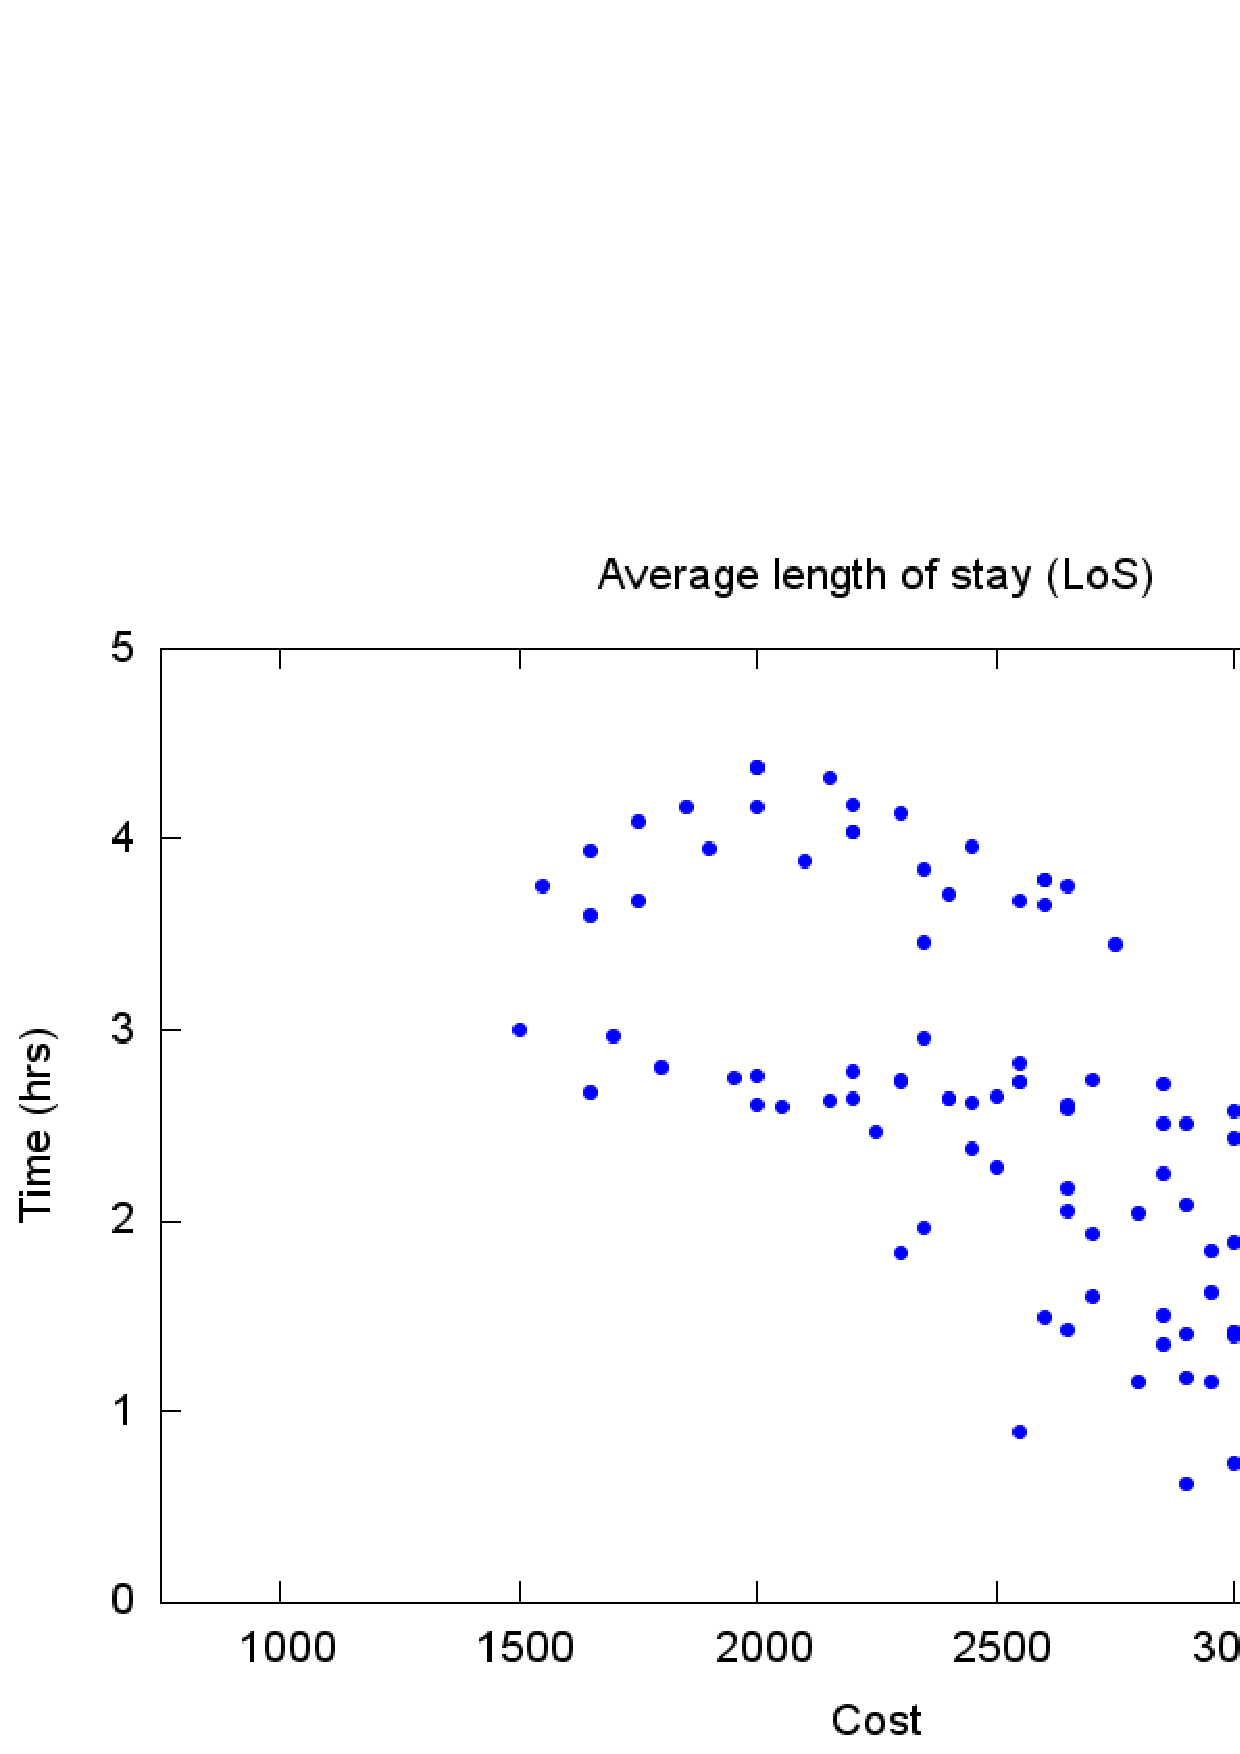
\includegraphics[width=0.95\columnwidth,height=0.25\paperheight]{figs4/v0/MC/MC-6400-602-50-69-25-125confs-LoS}\caption{Average LoS of 125 configurations obtained by the MC method. \label{subfig:mc13-1}}
\end{figure}
 However, it was difficult to get any conclusion about such region;
therefore, the complementary K-means method was performed. The K-means
method identified two different clusters, shown in \ref{subfig:km13-1}.
The most important was the green cluster (at the bottom right), which
delimited the region where the optimum was.
\begin{figure}[H]
\noindent \centering{}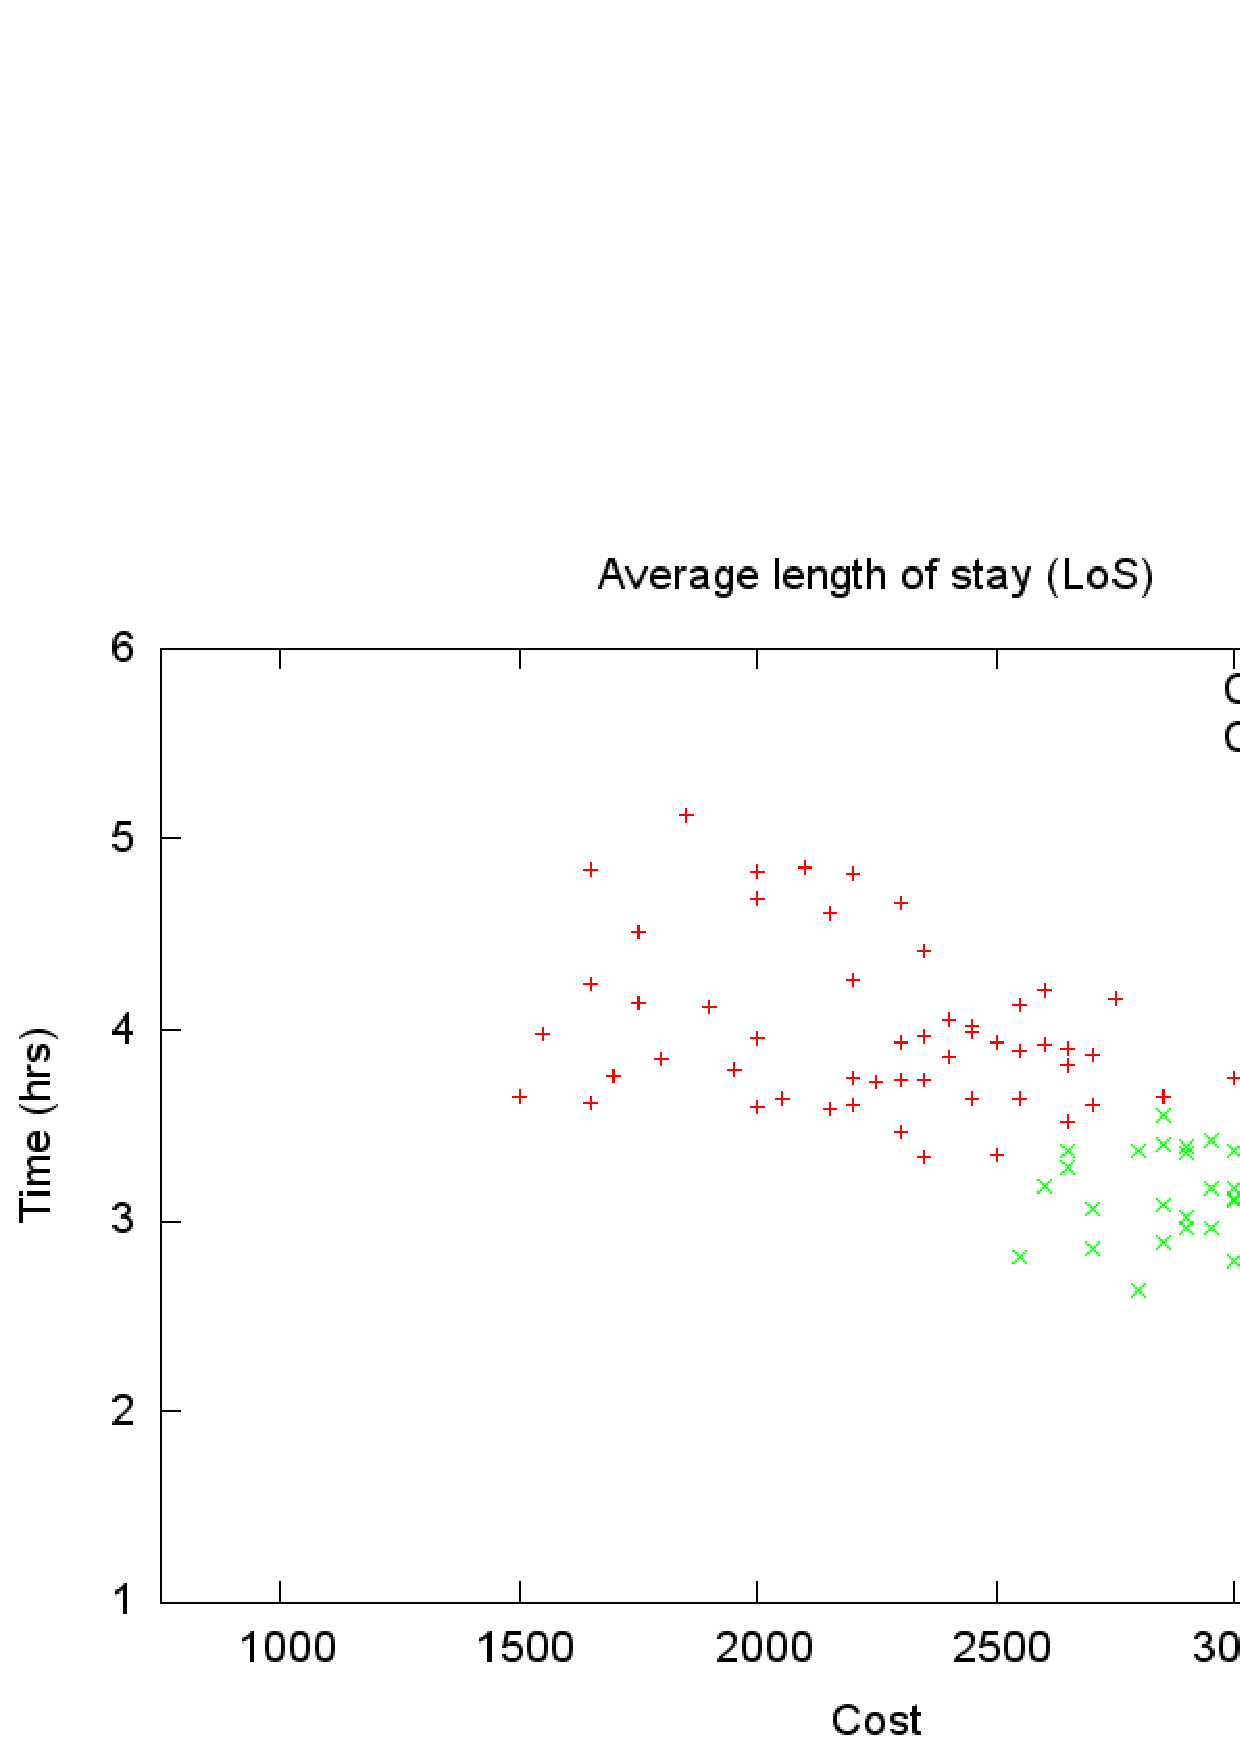
\includegraphics[width=0.95\columnwidth,height=0.25\paperheight]{figs4/v0/MC/K-means-6400-602-75-69-25-125-Cluster1-54_Cluster2-63}\caption{The K-means method identified two clusters of average LoS. The green
one delimited the region where the minimum was.\label{subfig:km13-1}}
\end{figure}


The \ref{fig:3D-scattered-graph-75} shows another way to visualise
the connectivity characteristic of the reduced regions found by the
the proposed methodology. The axes of such graph are the equivalent
operational patient-service time \foreignlanguage{american}{(t{*})}
of a ``single one'' sanitary professional of each sanitary staff
configuration (the first column of \ref{subtab:As-pipe} to \ref{subtab:Ds-pipe},
where they were ordered by the PA \ref{eq:Pipeline formula}). In
such figure, the points of interest were the green points, which lie
in the region of interest, where the minimum was, which can be seen
in black triangle. It can be seen that it was not necessary to search
in the whole feasible region, but only in the green connected region.
\begin{figure}[h]
\noindent \centering{}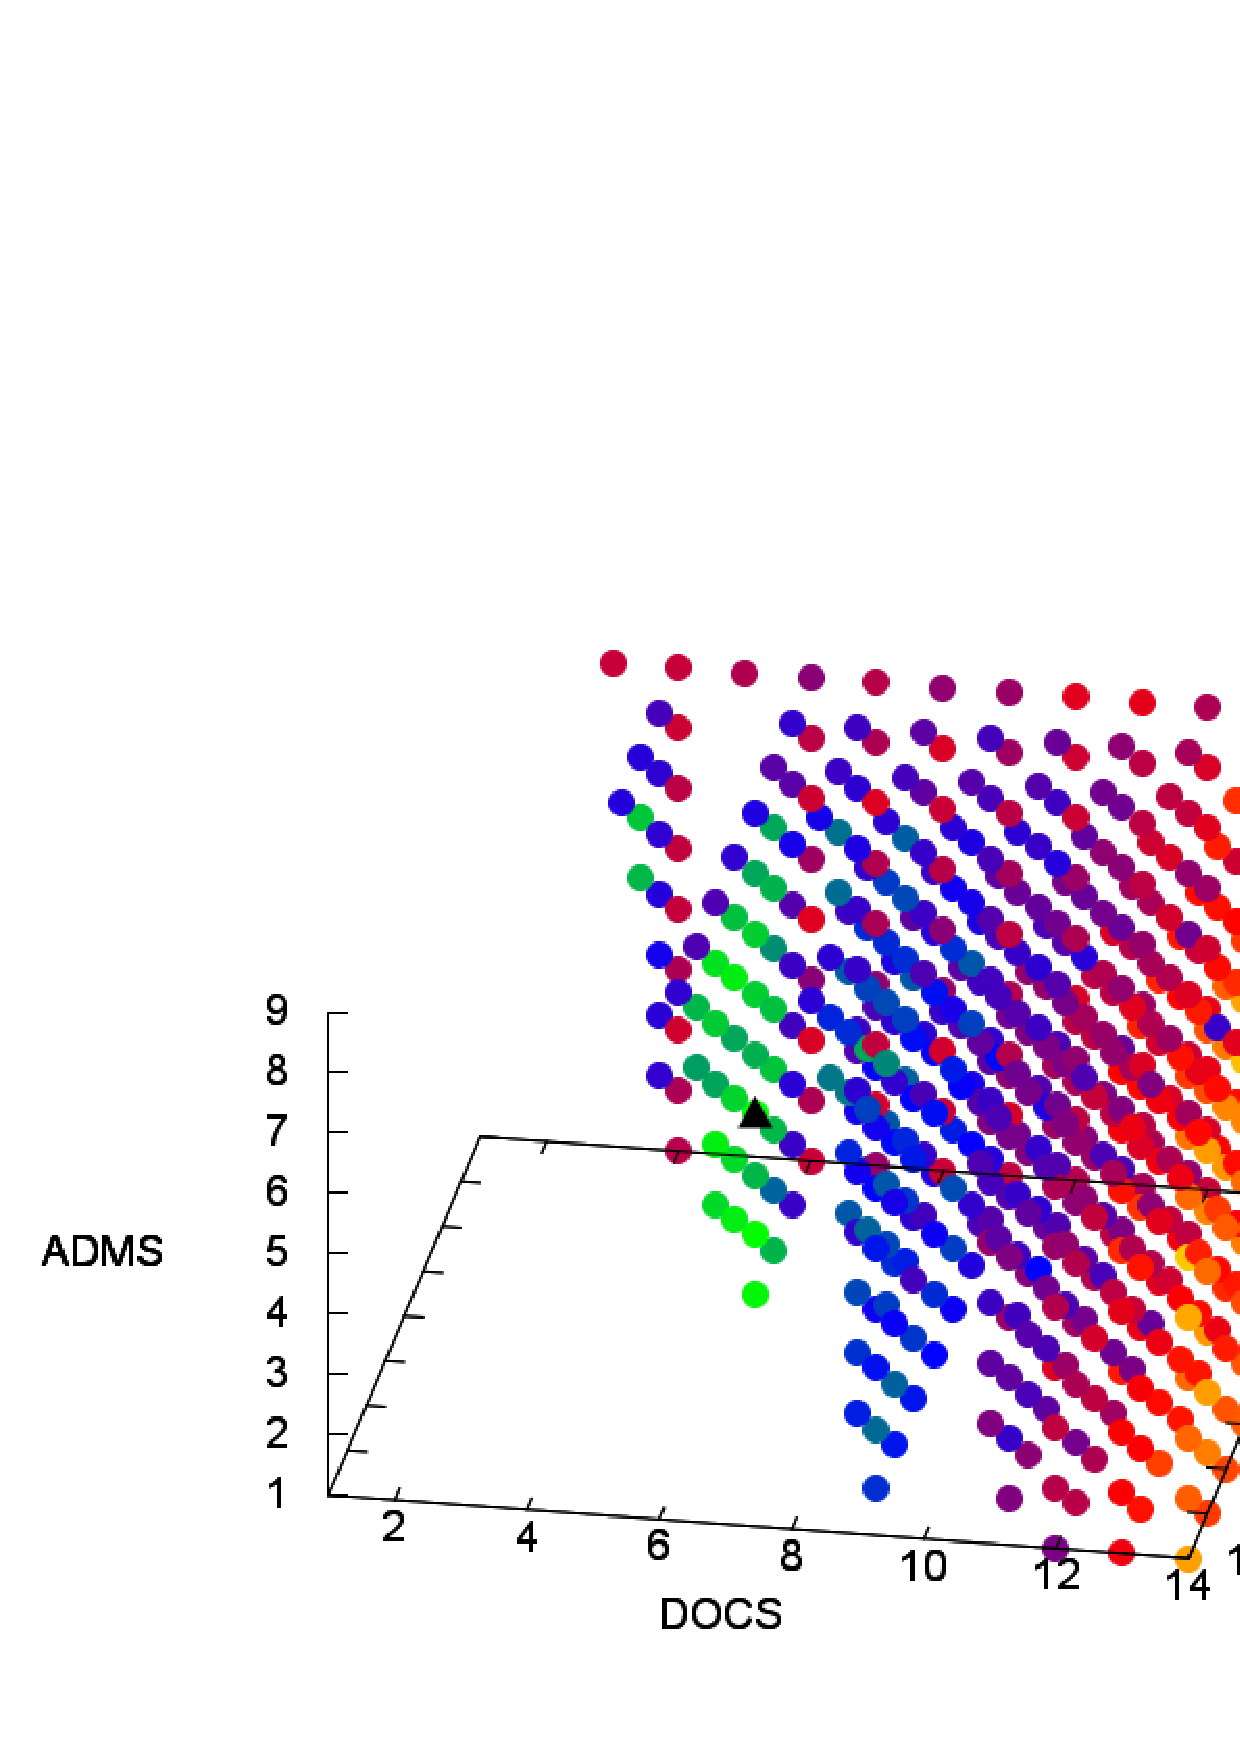
\includegraphics[width=0.88\columnwidth,height=0.2\paperheight]{figs4/v0/6400-602-75-3D-scatter-LoS2}\caption{3D scattered graph shows the average LoS index of the third workload
scenario (13 patients/hour). The average LoS index is expressed in
colour in hours. \label{fig:3D-scattered-graph-75}}
\end{figure}


Finally, after separately applied both the PA and the MC plus the
K-means methods, the \textquotedblleft{}reduced exhaustive search\textquotedblright{}
was separately performed in each reduced region identified. The optimum
found per each method: the ES, the PA, and the MC plus the K-means
methods are presented in \ref{tab:12p-a}, where the sanitary staff
configuration (doctors, nurses, and admission personnel), their associated
average minimum LoS, and cost configuration are shown. The three optima
independently found were the same. 

\begin{comment}
Each staff configuration that got the minimum is presented in \ref{tab:4p-a},
\ref{tab:8p-a}, \ref{tab:12p-a}, and \ref{tab:16p-a}.
\end{comment}
\vspace*{-.2cm}%
\begin{comment}
\begin{figure}[h]
\noindent \begin{centering}
\begin{minipage}[t][1\totalheight][s]{0.48\linewidth}%
\noindent \begin{center}
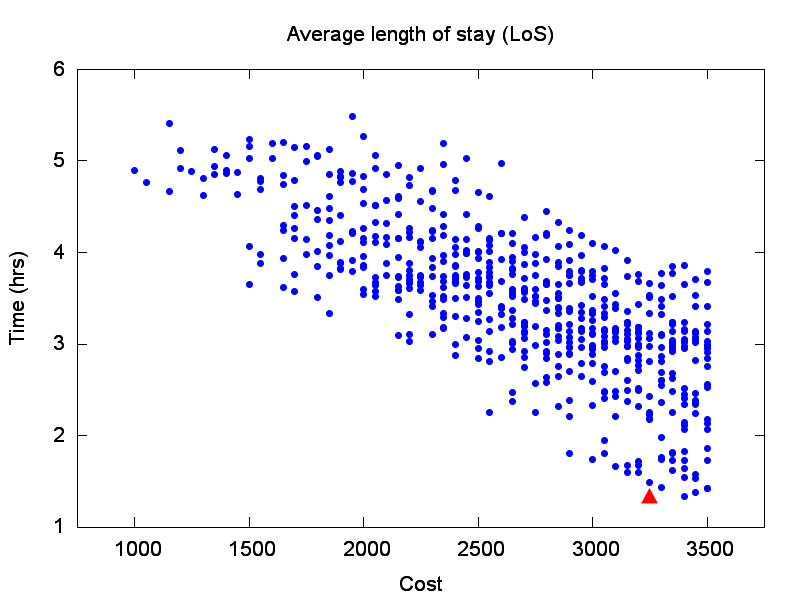
\includegraphics[width=1\columnwidth]{figs4/v0/6400-602-75-exh-LoS-min.png}
\par\end{center}

\vspace*{-1cm}

\noindent \begin{center}
\caption{Average LoS obtained by the ES method. The red triangle was the minimum.
\label{subfig:es12}}

\par\end{center}%
\end{minipage}\hfill{}%
\begin{minipage}[t][1\totalheight][s]{0.48\linewidth}%
\noindent \begin{center}
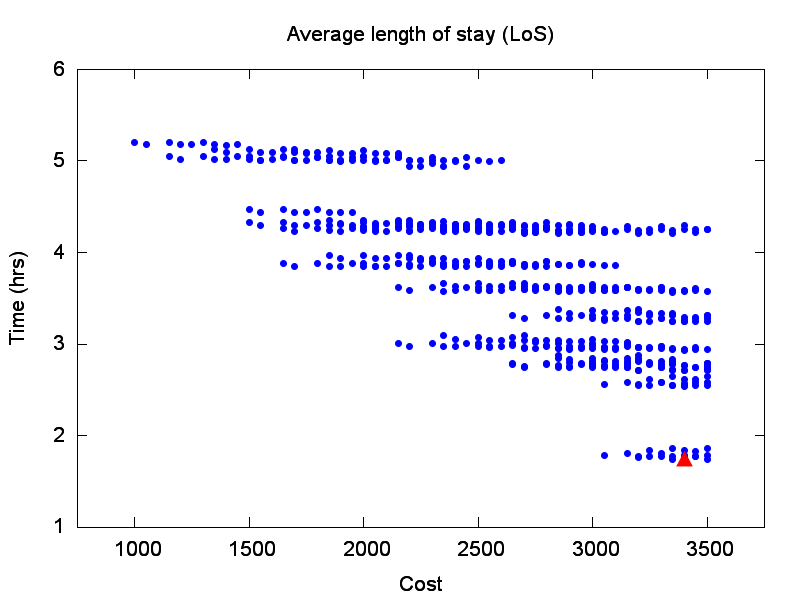
\includegraphics[width=1\columnwidth]{figs4/v0/pipe-sorted-LoS_0.75_min.png}
\par\end{center}

\vspace*{-1cm}

\noindent \begin{center}
\caption{Average LoS obtained by the PA. The red triangle was the minimum.\label{subfig:pipe12}}

\par\end{center}%
\end{minipage}
\par\end{centering}

\noindent \begin{centering}
%\centering\vspace{0cm}
\vspace*{-1.2cm}
\par\end{centering}

\begin{minipage}[t][1\totalheight][s]{0.48\textwidth}%
\noindent \begin{center}
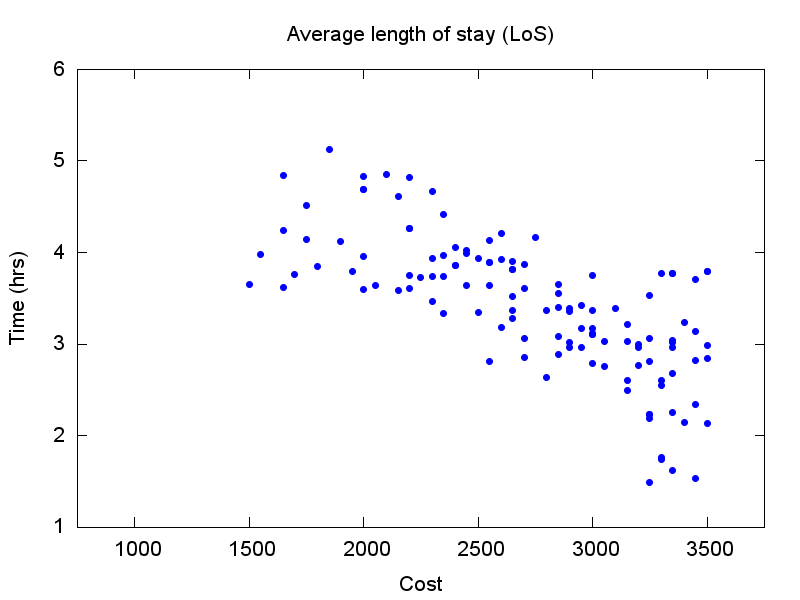
\includegraphics[width=1\columnwidth]{figs4/v0/MC/MC-6400-602-75-69-25-125confs-LoS.png}
\par\end{center}

\vspace*{-0.8cm}

\caption{Average LoS of 125 configurations obtained by the MC method.\label{subfig:mc12-1}}
%
\end{minipage}\hfill{}%
\begin{minipage}[t][1\totalheight][s]{0.48\textwidth}%
\noindent \begin{center}
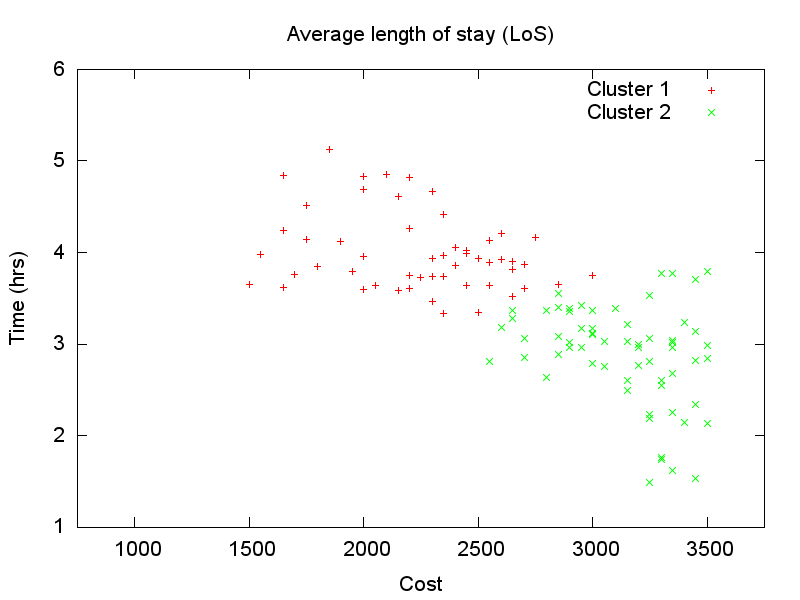
\includegraphics[width=1\columnwidth]{figs4/v0/MC/K-means-6400-602-75-69-25-125-Cluster1-54_Cluster2-63.png}
\par\end{center}

\vspace*{-0.8cm}

\caption{The K-means method identified two clusters of average LoS. The green
one delimited the region where the minimum was.\label{subfig:km12-1}}
%
\end{minipage}

\vspace*{0.4cm}{\bf Figures} show the average LoS of the third workload scenario (13 patients/hour) using the ES, the PA, and the MC+K-means methods.
\end{figure}
\end{comment}
\begin{comment}
\begin{figure}[h]
\hfill{}\subfloat[\label{subfloat:pipe12} Scattered 3D graph of doctors, nurses, and
admission personnel.]{

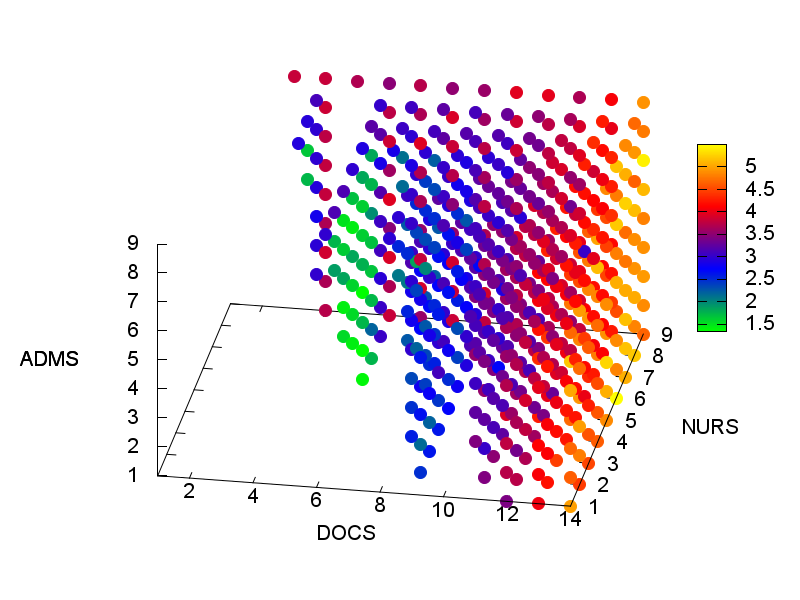
\includegraphics[width=0.48\columnwidth]{figs4/6400-602-75-3D-scatter-LoS.png}}\hfill{}\subfloat[\label{subfloat:contour12} Contour graph where doctors and nurses
can be seen.]{

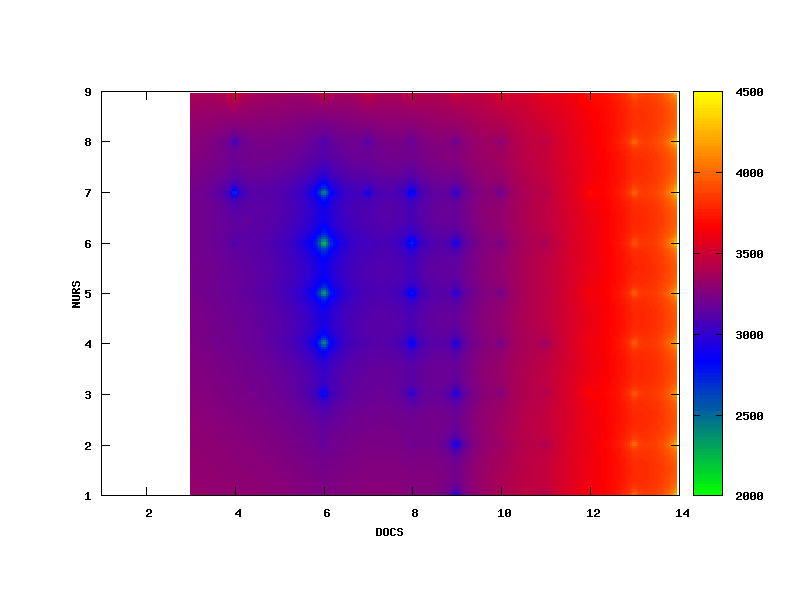
\includegraphics[width=0.48\columnwidth]{figs4/6400-602-75-sort-pipe_p5_y_p4-contour.png}}\hfill{}

\caption{\label{fig:Two-vision3} Graphs show the average LoS index of the
third workload scenario (13 patients/hour) using the first column
of \ref{subtab:As-pipe}, \ref{subtab:Ns-pipe}, and \ref{subtab:Ds-pipe},
where they were ordered by the pipeline approach (PA) \ref{eq:Pipeline formula}.
The colour bar is expresed in tics ( $hours\:=\frac{tics}{1000}$
). }
\end{figure}
\end{comment}


\begin{table}[h]
\caption{Optimum staff configurations that got the average minimum LoS for
this workload scenario (up to 13 patients hourly), where S is Senior
and J is Junior. This optimum sanitary staff configuration is shown
in red triangle in \ref{subfig:es13-1} and in black triangle in \ref{fig:3D-scattered-graph-75}.}


\begin{centering}
\begin{tabular}{cccccc>{\centering}p{2.8cm}}
\hline 
Method & � & LoS (hrs) & D & N & A & Run time (hrs)

4 Pthreads\tabularnewline
\hline 
ES & 3,250 & 1.33 & 4J & 1S,1J & 2S & 2.45\tabularnewline
PA & 3,250 & 1.33 & 4J & 1S,1J & 2S & 0.16\tabularnewline
MC+K-means & 3,250 & 1.33 & 4J & 1S,1J & 2S & 1.49\tabularnewline
\hline 
\end{tabular}
\par\end{centering}

\label{tab:12p-a} 
\end{table}


\clearpage{}


\subsubsection{Fourth Workload Scenario}

The results of this scenario, up to 17 patients/hour, are shown from
\ref{subfig:es17-1} to \ref{subfig:km17-1}. The ES result is shown
in \ref{subfig:es17-1}, where the red triangle is the minimum. 
\begin{figure}[H]
\noindent \begin{centering}
\includegraphics[width=0.95\columnwidth,height=0.25\paperheight]{figs4/v0/6400-602-100-exh-LoS-min}
\par\end{centering}

\caption{Average LoS obtained by the ES. The red triangle was the minimum.
\label{subfig:es17-1}}
\end{figure}


The PA result is shown in \ref{subfig:pipe17-1}, where many regions
can be clearly seen and the red triangle is the minimum.
\begin{figure}[H]
\noindent \begin{centering}
\includegraphics[width=0.95\columnwidth,height=0.25\paperheight]{figs4/v0/pipe-sorted-LoS_1\lyxdot 0_min}
\par\end{centering}

\caption{Average LoS obtained by the PA. The red triangle was the minimum.
\label{subfig:pipe17-1}}
\end{figure}
 The most important is the bottom region, in which the average minimum
LoS was around than 3 hours. There were 21 configurations (from a
total of 602 in the feasible region) in this region, which is the
one where the maximum was.

The MC plus the K-means methods results are shown in \ref{subfig:mc17-1}
to \ref{subfig:km17-1}, respectively. The MC method found 125 configurations.
\begin{figure}[H]
\noindent \centering{}\includegraphics[width=0.95\columnwidth,height=0.25\paperheight]{figs4/v0/MC/MC-6400-602-100-69-25-125confs-LoS}\caption{Average LoS of 125 configurations obtained by the MC method. \label{subfig:mc17-1}}
\end{figure}
 However, it was difficult to get any conclusion about such region;
therefore, the complementary K-means method was performed. The K-means
method identified two different clusters, shown in \ref{subfig:km17-1}.
The most important was the green cluster (at the bottom right), which
delimited the region where the optimum was.
\begin{figure}[H]
\noindent \centering{}\includegraphics[width=0.95\columnwidth,height=0.25\paperheight]{figs4/v0/MC/K-means-6400-602-100-69-25-125-Cluster1-49_Cluster2-68}\caption{The K-means method identified two clusters of average LoS. The green
one delimited the region where the minimum was.\label{subfig:km17-1}}
\end{figure}


The \ref{fig:3D-scattered-graph-100} shows another way to visualise
the connectivity characteristic of the reduced regions found by the
proposed methodology. The axes of such graph are the equivalent operational
patient-service time \foreignlanguage{american}{(t{*})} of a ``single
one'' sanitary professional of each sanitary staff configuration
(the first column of \ref{subtab:As-pipe} to \ref{subtab:Ds-pipe},
where they were ordered by the PA \ref{eq:Pipeline formula}). In
such figure, the points of interest were the green points, which lie
in the region of interest, where the minimum was, which can be seen
in black triangle. It can be seen that it was not necessary to search
in the whole feasible region, but only in the green connected region.
\begin{figure}[h]
\noindent \centering{}\includegraphics[width=0.88\columnwidth,height=0.2\paperheight]{figs4/v0/6400-602-100-3D-scatter-LoS2}\caption{3D scattered graph shows the average LoS index of the third workload
scenario (17 patients/hour). The average LoS index is expressed in
colour in hours. \label{fig:3D-scattered-graph-100}}
\end{figure}


Finally, after separately applied both the PA and the MC plus the
K-means methods, the \textquotedblleft{}reduced exhaustive search\textquotedblright{}
was separately performed in each reduced region identified.The optimum
found per each method: the ES, the PA, and the MC plus the K-means
methods are presented in \ref{tab:16p-a}, where the sanitary staff
configuration (doctors, nurses, and admission personnel), their associated
average minimum LoS, and cost configuration are shown. The three optima
independently found were the same. 

\begin{comment}
Each staff configuration that got the minimum is presented in \ref{tab:4p-a},
\ref{tab:8p-a}, \ref{tab:12p-a}, and \ref{tab:16p-a}.
\end{comment}
\vspace*{-.2cm}%
\begin{comment}
\begin{figure}[h]
\noindent \begin{centering}
\begin{minipage}[t][1\totalheight][s]{0.48\linewidth}%
\noindent \begin{center}
\includegraphics[width=1\columnwidth]{figs4/v0/6400-602-100-exh-LoS-min.png}
\par\end{center}

\vspace*{-1cm}

\noindent \begin{center}
\caption{Average LoS obtained by the ES method. The red triangle was the minimum.\label{subfig:es16}}

\par\end{center}%
\end{minipage}\hfill{}%
\begin{minipage}[t][1\totalheight][s]{0.48\linewidth}%
\noindent \begin{center}
\includegraphics[width=1\columnwidth]{figs4/v0/pipe-sorted-LoS_1.0_min.png}
\par\end{center}

\vspace*{-1cm}

\noindent \begin{center}
\caption{Average LoS obtained by the PA. The red triangle was the maximum.\label{subfig:pipe16}}

\par\end{center}%
\end{minipage}
\par\end{centering}

\noindent \begin{centering}
%\centering\vspace{0cm}
\vspace*{-1.2cm}
\par\end{centering}

\begin{minipage}[t][1\totalheight][s]{0.48\textwidth}%
\noindent \begin{center}
\includegraphics[width=1\columnwidth]{figs4/v0/MC/MC-6400-602-100-69-25-125confs-LoS.png}
\par\end{center}

\vspace*{-0.8cm}

\caption{Average LoS of 125 configurations obtained by the MC method. \label{subfig:mc16-1}}
%
\end{minipage}\hfill{}%
\begin{minipage}[t][1\totalheight][s]{0.48\textwidth}%
\noindent \begin{center}
\includegraphics[width=1\columnwidth]{figs4/v0/MC/K-means-6400-602-100-69-25-125-Cluster1-49_Cluster2-68.png}
\par\end{center}

\vspace*{-0.8cm}

\caption{The K-means method identified two clusters of average number of attended
patients. The green one delimited the region where the minimum was.\label{subfig:km16-1}}
%
\end{minipage}

\vspace*{0.4cm}{\bf Figures} show the average LoS of the fourth workload scenario (17 patients/hour) using the ES, the PA, and the MC+K-means methods.
\end{figure}
\end{comment}
\begin{comment}
\begin{figure}[h]
\hfill{}\subfloat[\label{subfloat:pipe16} Scattered 3D graph of doctors, nurses, and
admission personnel.]{

\includegraphics[width=0.48\columnwidth]{figs4/6400-602-100-3D-scatter-LoS.png}}\hfill{}\subfloat[\label{subfloat:contour16} Contour graph where doctors and nurses
can be seen.]{

\includegraphics[width=0.48\columnwidth]{figs4/6400-602-100-sort-pipe_p5_y_p4-contour.png}}\hfill{}

\caption{\label{fig:Two-vision4} Graphs show the average LoS index of the
fourth workload scenario (17 patients/hour) using the first column
of \ref{subtab:As-pipe}, \ref{subtab:Ns-pipe}, and \ref{subtab:Ds-pipe},
where they were ordered by the pipeline approach (PA) \ref{eq:Pipeline formula}.
The colour bar is expresed in tics ( $hours\:=\frac{tics}{1000}$
). }
\end{figure}
\end{comment}
%\hspace{6cm}
%\vspace{-.5cm}


\begin{table}[h]
\caption{Optimum staff configurations that got the average minimum LoS for
this workload scenario (up to 17 patients hourly), where S is Senior
and J is Junior. This optimum sanitary staff configuration is shown
in red triangle in \ref{subfig:es17-1} and in black triangle in \ref{fig:3D-scattered-graph-100}.}


\begin{centering}
\begin{tabular}{cccccc>{\centering}p{2.8cm}}
\hline 
Method & � & LoS (hrs) & D & N & A & Run time (hrs)

4 Pthreads\tabularnewline
\hline 
ES & 3,450  & 2.3  & 4J & 3J & 2S & 3.42\tabularnewline
PA & 3,450 & 2.3 & 4J & 3J & 2S & 0.15\tabularnewline
MC+K-means & 3,450  & 2.3  & 4J & 3J & 2S & 2.0\tabularnewline
\hline 
\end{tabular}
\par\end{centering}

\label{tab:16p-a} 
\end{table}


\begin{comment}
In the other cases, where the patient arrival increases there are
only few staff configurations around the minimum, or clearly only
one. But not only the patient arrival increases, but also the minimum
average patient stay time, as expected, but also the standard deviation,
patients at waiting rooms, both WR0 and WR1 at times t1, t2, t3, and
t4, and finally the amount of unattended patients increases too. In
\ref{tab:20_40_60_80_I1} all these results are shown. In Figure \ref{fig:exp1_WR}
the amount of patients in WR are shown, WR0 plus WR1, at four different
moments, t1=6,000, t2=12,000, t3=18,000, t4=24,000, during the simulation
for all the seven cases reported. It is noticed when the patient arrival
is high, 17 per hour, patients at waiting rooms increased.

%\hspace{6cm}
%\vspace{-.5cm}


\begin{table}[h]
\caption{Results for the best average minimum for each of the four presented
scenarios.}


{\small{\addtolength{\tabcolsep}{-5pt} }}{\small \par}

\begin{centering}
\resizebox{5.5in}{!}{{\small{}}%
\begin{tabular}{|c|c|c|c|c|c|c|c|}
\hline 
\multicolumn{1}{|c|}{{\small{P}}} & \multicolumn{1}{c|}{{\small{T1 }}} & \multicolumn{1}{c|}{{\small{ $\sigma$ }}} & \multicolumn{1}{c|}{{\small{Euros }}} & \multicolumn{1}{c|}{{\small{\# attended }}} & \multicolumn{1}{c|}{{\small{\# unattended }}} & {\small{WR0 }} & {\small{WR1 }}\tabularnewline
\cline{7-8} 
\multicolumn{1}{|c|}{} & \multicolumn{1}{c|}{} & \multicolumn{1}{c|}{} & \multicolumn{1}{c|}{} & \multicolumn{1}{c|}{{\small{patients}}} & \multicolumn{1}{c|}{{\small{patients}}} & {\small{t1, t2, t3, t4 }} & {\small{t1, t2, t3, t4 }}\tabularnewline
\hline 
{\small{4 }} & {\small{428 }} & {\small{48 (11\%) }} & {\small{2,850 }} & {\small{83 }} & {\small{1 }} & {\small{0,0,0,0 }} & {\small{0,0,0,0 }}\tabularnewline
\hline 
9 & {\small{514 }} & {\small{81.5 (15.9\%) }} & {\small{3,150 }} & {\small{182 }} & {\small{4 }} & {\small{0,0,0,1 }} & {\small{0,0,0,0 }}\tabularnewline
\hline 
{\small{13 }} & {\small{790 }} & {\small{174.5 (22.1\%) }} & {\small{3,400 }} & {\small{290 }} & {\small{8 }} & {\small{1,1,0,1 }} & {\small{3,2,4,1 }}\tabularnewline
\hline 
{\small{17 }} & {\small{3266 }} & {\small{1670.4 (51.2\%) }} & {\small{3,350 }} & {\small{294 }} & {\small{100 }} & {\small{8,19,32,43 }} & {\small{12,25,37,51 }}\tabularnewline
\hline 
\end{tabular}{\small{}}}
\par\end{centering}{\small \par}

{\small{\label{tab:20_40_60_80_I1}}}
\end{table}
\end{comment}
\clearpage{}


\subsection{Throughput Index}

The second objective set was to maximise number of attended patients
per day (Throughput) in the ED, with cost configuration constraint
less or equal to 3,500 �. This index is expressed mathematically in
\ref{eq:Throughput index}:\vspace*{-0.125cm}
\begin{equation}
\begin{aligned} & {\text{Maximise patients attended}} &  & f(D,N,A)\\
 & \text{subject to} &  & D_{cost}+N_{cost}+A_{cost}\in Cost\leq3,500\:\text{�}
\end{aligned}
\label{eq:Throughput index}
\end{equation}


It is worth noting that each of the plotted points were obtained running
the ED simulator as many times as points are. Each plotted point corresponds
to each of the 602 staff configurations (out of 1,134) that satisfy
the cost restriction.


\subsubsection{First Workload Scenario}

The results of this scenario, up to 4 patients/hour, are shown from
\ref{subfig:es4-2} to \ref{subfig:km4-2}. \ref{subfig:es4-2} shows
ES results. The red triangles were the maxima.
\begin{figure}[H]
\centering{}\vspace*{-0.2cm}\includegraphics[width=0.9\columnwidth,height=0.19\paperheight]{figs4/v0\lyxdot 2/6400-602-25-exh-throughput-max}\caption{Average number of attended patients obtained by the ES method. The
red triangles were the maxima. \label{subfig:es4-2}}
\end{figure}
 \vspace*{-0.2cm}

\begin{figure}[H]
\centering{}\vspace*{-0.2cm}\includegraphics[width=0.9\columnwidth,height=0.19\paperheight]{figs4/v0\lyxdot 2/pipe-sorted-Throughput_0\lyxdot 25_max}\caption{Average number of attended patients obtained by the PA. The red triangles
were the maxima. \label{subfig:pipe4-2}}
\end{figure}
 The PA result is shown in \ref{subfig:pipe4-2}, where three regions
can be clearly seen and the red triangles were the maxima. The most
important is the top region, in which the average maximum Throughput
was more than 80 attended patients. There were 440 configurations
(from a total of 602 in the feasible region) in this region, which
was the one where the maxima were.

The MC plus the K-means methods results are shown in \ref{subfig:mc4-2}
to \ref{subfig:km4-2}, respectively. The MC method found 50 configurations.
\begin{figure}[H]
\centering{}\vspace*{-0.2cm}\includegraphics[width=0.9\columnwidth,height=0.22\paperheight]{figs4/v0\lyxdot 2/MC/MC-6400-602-25-69-25-50confs-Throughput}\caption{Average number of attended patients of 50 configurations obtained
by the MC method.\label{subfig:mc4-2}}
\end{figure}
However, it was difficult to get any conclusion about such region;
therefore, the complementary K-means method was performed. The K-means
method identified two different clusters, shown in \ref{subfig:km4-2}.
The most important was the green cluster, which delimited the region
where the optima were.
\begin{figure}[H]
\begin{centering}
\vspace*{-0.2cm}\includegraphics[width=0.9\columnwidth,height=0.22\paperheight]{figs4/v0\lyxdot 2/MC/K-means-6400-602-25-69-25-50-Cluster1-23_Cluster2-25}
\par\end{centering}

\caption{The K-means method identified two clusters of average number of attended
patients. The green one delimited the region where the maxima were.\label{subfig:km4-2}}
\end{figure}


\begin{comment}
The graphics \ref{subfloat:pipe4} and \ref{subfloat:contour4} shown
another way to visualise the connectivity characteristic of the reduced
regions found by the AP, and the MC plus the K-means methods. In such
connected reduced regions the ``reduced exhaustive search'' is applied.
The axes of such graphs are the first column of \ref{subtab:As-pipe},
\ref{subtab:Ns-pipe}, and \ref{subtab:Ds-pipe}, where they were
ordered by the pipeline approach (PA) \ref{eq:Pipeline formula}.
\end{comment}


Finally, after separately applied both the PA and the MC plus the
K-means methods, the \textquotedblleft{}reduced exhaustive search\textquotedblright{}
was separately performed in each reduced region identified. The optimum
found per each method: the ES, the PA, and the MC plus the K-means
methods are presented in \ref{tab:4p-b}, where the sanitary staff
configuration (doctors, nurses, and admission personnel), their associated
average maximum Throughput, and cost configuration are shown. The
three optima independently found were the same. 
\begin{table}[H]
\caption{Optimum staff configurations that got the average maximum Throughput
for this workload scenario (up to 4 patients hourly), where S is Senior
and J is Junior. These optimum sanitary staff configurations are shown
in red triangle in \ref{subfig:es4-2}.}


\begin{centering}
\begin{tabular}{cc>{\centering}p{2cm}ccc>{\centering}p{2.8cm}}
\hline 
Method & � & \#attended patients & D & N & A & Run time (hrs)

4 Pthreads\tabularnewline
\hline 
ES & 3,050 & 86 & 2S & 1S,1J & 1S & 0.91\tabularnewline
PA & 3,050 & 86 & 2S & 1S,1J & 1S & 0.63\tabularnewline
MC+K-means & 3,050 & 86 & 2S & 1S,1J & 1S & 0.73\tabularnewline
\hline 
\end{tabular}
\par\end{centering}

\label{tab:4p-b} 
\end{table}


\begin{comment}
The results are shown in the Figure \ref{fig:exp2_80}, where the
blue points are the staff configuration that satisfy the restriction,
while the red point is the minimum. Its configuration is presented
in Table \ref{2o_I_80_20}. It order to get the same time or less,
the superior limit for staff members was increased to: $doctors<9$;
$nurses<7$, and $admissions<5$. This index can be seen as looking
for a staff configuration that guarantee, at least, the same quality
for high patient arrival, 17 per hour, as the same that was gotten
for low patient arrival, 4 per hour.
\end{comment}
\begin{comment}
\begin{figure}[h]
\noindent \begin{centering}
\begin{minipage}[t][1\totalheight][s]{0.48\columnwidth}%
\noindent \begin{center}
\includegraphics[width=1\columnwidth]{figs4/v0.2/6400-602-25-exh-throughput-max.png}
\par\end{center}

\vspace*{-1cm}

\noindent \begin{center}
\caption{Average number of attended patients obtained by the ES method. The
red triangles were the maximum. }

\par\end{center}%
\end{minipage}\hfill{}%
\begin{minipage}[t][1\totalheight][s]{0.48\columnwidth}%
\noindent \begin{center}
\includegraphics[width=1\columnwidth]{figs4/v0.2/pipe-sorted-Throughput_0.25_max.png}
\par\end{center}

\vspace*{-1cm}

\noindent \begin{center}
\caption{Average number of attended patients obtained by the PA. The red triangles
were the maximum. }

\par\end{center}%
\end{minipage}
\par\end{centering}

\noindent \begin{centering}
%\centering\vspace{0cm}
\vspace*{-1.2cm}
\par\end{centering}

\begin{minipage}[t][1\totalheight][s]{0.48\columnwidth}%
\noindent \begin{center}
\includegraphics[width=1\columnwidth]{figs4/v0.2/MC/MC-6400-602-25-69-25-50confs-Throughput-TRI.pdf}
\par\end{center}

\vspace*{-0.8cm}

\caption{Average number of attended patients of 50 configurations obtained
by the MC method. }
%
\end{minipage}\hfill{}%
\begin{minipage}[t][1\totalheight][s]{0.48\columnwidth}%
\noindent \begin{center}
\includegraphics[width=1\columnwidth]{figs4/v0.2/MC/K-means-6400-602-25-69-25-50-Cluster1-23_Cluster2-25_TRI.pdf}
\par\end{center}

\vspace*{-0.8cm}

\caption{The K-means method identified two clusters of average number of attended
patients. The green one delimited the region where the maximum were.}
%
\end{minipage}

\vspace*{0.4cm}{\bf Figures} show the average Throughput of the first workload scenario (4 patients/hour) using the ES, the PA, and the MC+K-means methods.
\end{figure}
\end{comment}


\begin{comment}
From Figures \ref{fig:exp1_20} and \ref{tab:4p-b}, there is a staff
configuration that got the minimum time. Also, in such Figures \ref{fig:exp1_20}
can appreciate that there are many other staff configurations that
are quite close to the optimum, but with less cost.
\end{comment}



\subsubsection{Second Workload Scenario}

The results of this scenario, up to 9 patients/hour, are shown from
\ref{subfig:es8-2} to \ref{subfig:km8-2}. The ES result is shown
in \ref{subfig:es8-2}, where the red triangle was the maximum. 
\begin{figure}[H]
\centering{}\includegraphics[width=0.95\columnwidth,height=0.25\paperheight]{figs4/v0\lyxdot 2/6400-602-50-exh-throughput-max}\caption{Average number of attended patients obtained by the ES method. The
red triangle was the maximum.\label{subfig:es8-2}}
\end{figure}


The PA result is shown in \ref{subfig:pipe8-2}, where many regions
can be seen and the red triangle was the maximum. 
\begin{figure}[H]
\centering{}\includegraphics[width=0.95\columnwidth,height=0.25\paperheight]{figs4/v0\lyxdot 2/pipe-sorted-Throughput_0\lyxdot 50_max}\caption{Average number of attended patients obtained by the PA. The red triangles
were the maximum.\label{subfig:pipe8-2}}
\end{figure}
 The most important is the top region, in which the average maximum
Throughput was more than 150 attended patients. There were 180 configurations
(from a total of 602 in the feasible region) in this region, which
was the one where the maximum was.

The MC plus the K-means methods results are shown in \ref{subfig:mc8-2}
to \ref{subfig:km8-2}, respectively. The MC method found 125 configurations.
\begin{figure}[H]
\centering{}\includegraphics[width=0.95\columnwidth,height=0.25\paperheight]{figs4/v0\lyxdot 2/MC/MC-6400-602-50-69-25-125confs-Throughput}\caption{Average number of attended patients of 125 configurations obtained
by the MC method. \label{subfig:mc8-2}}
\end{figure}
 However, it was difficult to get any conclusion about such region;
therefore, the complementary K-means method was performed. The K-means
method identified two different clusters, shown in \ref{subfig:km8-2}.
The most important was the green cluster, which delimited the region
where the optimum was.
\begin{figure}[H]
\begin{centering}
\includegraphics[width=0.95\columnwidth,height=0.25\paperheight]{figs4/v0\lyxdot 2/MC/K-means-6400-602-50-69-25-125-Cluster1-56_Cluster2-60}
\par\end{centering}

\caption{The K-means method identified two clusters of average number of attended
patients. The green one delimited the region where the maximum was.\label{subfig:km8-2}}
\end{figure}


\begin{comment}
The graphics \ref{subfloat:pipe4} and \ref{subfloat:contour4} shown
another way to visualise the connectivity characteristic of the reduced
regions found by the AP, and the MC plus the K-means methods. In such
connected reduced regions the ``reduced exhaustive search'' is applied.
The axes of such graphs are the first column of \ref{subtab:As-pipe},
\ref{subtab:Ns-pipe}, and \ref{subtab:Ds-pipe}, where they were
ordered by the pipeline approach (PA) \ref{eq:Pipeline formula}.
\end{comment}


Finally, after separately applied both the PA and the MC plus the
K-means methods, the \textquotedblleft{}reduced exhaustive search\textquotedblright{}
was separately performed in each reduced region identified. The optimum
found per each method: the ES, the PA, and the MC plus the K-means
methods are presented in \ref{tab:8p-b}, where the sanitary staff
configuration (doctors, nurses, and admission personnel), their associated
average maximum Throughput, and cost configuration are shown. The
three optima independently found were the same.

\begin{comment}
\begin{figure}[h]
\noindent \begin{centering}
\begin{minipage}[t][1\totalheight][s]{0.48\columnwidth}%
\noindent \begin{center}
\includegraphics[width=1\columnwidth]{figs4/v0.2/6400-602-50-exh-throughput-max.png}
\par\end{center}

\vspace*{-1cm}

\noindent \begin{center}
\caption{}

\par\end{center}%
\end{minipage}\hfill{}%
\begin{minipage}[t][1\totalheight][s]{0.48\columnwidth}%
\noindent \begin{center}
\includegraphics[width=1\columnwidth]{figs4/v0.2/pipe-sorted-Throughput_0.50_max.png}
\par\end{center}

\vspace*{-1cm}

\noindent \begin{center}
\caption{}

\par\end{center}%
\end{minipage}
\par\end{centering}

\noindent \begin{centering}
%\centering\vspace{0cm}
\vspace*{-1.2cm}
\par\end{centering}

\begin{minipage}[t][1\totalheight][s]{0.48\columnwidth}%
\noindent \begin{center}
\includegraphics[width=1\columnwidth]{figs4/v0.2/MC/MC-6400-602-50-69-25-125confs-Throughput.png}
\par\end{center}

\vspace*{-0.8cm}

\caption{}
%
\end{minipage}\hfill{}%
\begin{minipage}[t][1\totalheight][s]{0.48\columnwidth}%
\noindent \begin{center}
\includegraphics[width=1\columnwidth]{figs4/v0.2/MC/K-means-6400-602-50-69-25-125-Cluster1-56_Cluster2-60.png}
\par\end{center}

\vspace*{-0.8cm}

\caption{}
%
\end{minipage}

\vspace*{0.4cm}{\bf Figures} show the average Throughput of the second workload scenario (9 patients/hour) using the ES, the PA, and the MC+K-means methods.
\end{figure}
\end{comment}


\begin{table}[H]
\caption{Optimum staff configurations that got the average maximum Throughput
for this workload scenario (up to 9 patients hourly), where S is Senior
and J is Junior. These optimum sanitary staff configurations are shown
in red triangle in \ref{subfig:es8-2}.}


\begin{centering}
\begin{tabular}{cc>{\centering}p{2cm}ccc>{\centering}p{2.8cm}}
\hline 
Method & � & \#attended patients & D & N & A & Run time (hrs)

4 Pthreads\tabularnewline
\hline 
ES & 3,350 & 163 & 1S,2J & 2S & 1S,1J & 1.59\tabularnewline
PA & 3,350 & 163 & 1S,2J & 2S & 1S,1J & 0.39\tabularnewline
MC+K-means & 3,350 & 163 & 1S,2J & 2S & 1S,1J & 1.08\tabularnewline
\hline 
\end{tabular}
\par\end{centering}

\label{tab:8p-b} 
\end{table}



\subsubsection{Third Workload Scenario}

The results of this scenario, up to 13 patients/hour, are shown from
\ref{subfig:es12-2} to \ref{subfig:km12-2}. The ES result is shown
in \ref{subfig:es12-2}, where the red triangle was the maximum. 

The PA result is shown in \ref{subfig:pipe12-2}, many regions can
be seen and the red triangle was the maximum. The most important is
the top region, in which the average maximum Throughput was more than
200 attended patients. There were 21 configurations (from a total
of 602 in the feasible region) in this region, which is the one where
the maximum was.

\begin{figure}[H]
\centering{}\includegraphics[width=0.95\columnwidth,height=0.25\paperheight]{figs4/v0\lyxdot 2/6400-602-75-exh-throughput-max}\caption{Average number of attended patients obtained by the ES method. The
red triangle was the maximum. \label{subfig:es12-2}}
\end{figure}
 
\begin{figure}[H]
\centering{}\includegraphics[width=0.95\columnwidth,height=0.25\paperheight]{figs4/v0\lyxdot 2/pipe-sorted-Throughput_0\lyxdot 75_max}\caption{Average number of attended patients obtained by the PA. The red triangles
were the maximum.\label{subfig:pipe12-2}}
\end{figure}


The MC plus the K-means methods results are shown in \ref{subfig:mc12-2}
to \ref{subfig:km12-2}, respectively. The MC method found 275 configurations.
\begin{figure}[H]
\centering{}\includegraphics[width=0.95\columnwidth,height=0.25\paperheight]{figs4/v0\lyxdot 2/MC/MC-6400-602-75-69-25-275confs-Throughput}\caption{Average number of attended patients of 275 configurations obtained
by the MC method. \label{subfig:mc12-2}}
\end{figure}
 However, it was difficult to get any conclusion about such region;
therefore, the complementary K-means method was performed. The K-means
method identified two different clusters, shown in \ref{subfig:km12-2},
the most important was the green cluster, which delimited the region
where the optimum was.
\begin{figure}[H]
\begin{centering}
\includegraphics[width=0.95\columnwidth,height=0.25\paperheight]{figs4/v0\lyxdot 2/MC/K-means-6400-602-75-69-25-275-Cluster1-91_Cluster2-123}
\par\end{centering}

\caption{The K-means method identified two clusters of average number of attended
patients. The green one delimited the region where the maximum was.\label{subfig:km12-2}}
\end{figure}


\begin{comment}
The graphics \ref{subfloat:pipe4} and \ref{subfloat:contour4} shown
another way to visualise the connectivity characteristic of the reduced
regions found by the AP, and the MC plus the K-means methods. In such
connected reduced regions the ``reduced exhaustive search'' is applied.
The axes of such graphs are the first column of \ref{subtab:As-pipe},
\ref{subtab:Ns-pipe}, and \ref{subtab:Ds-pipe}, where they were
ordered by the pipeline approach (PA) \ref{eq:Pipeline formula}.
\end{comment}


Finally, after separately applied both the PA and the MC plus the
K-means methods, the \textquotedblleft{}reduced exhaustive search\textquotedblright{}
was separately performed in each reduced region identified. The optimum
found per each method: the ES, the PA, and the MC plus the K-means
methods are presented in \ref{tab:12p-b}, where the sanitary staff
configuration (doctors, nurses, and admission personnel), and their
associated average maximum Throughput, and cost configuration are
shown. The three optima independently found were the same.

\begin{comment}
\begin{figure}[h]
\noindent \begin{centering}
\begin{minipage}[t][1\totalheight][s]{0.48\columnwidth}%
\noindent \begin{center}
\includegraphics[width=1\columnwidth]{figs4/v0.2/6400-602-75-exh-throughput-max.png}
\par\end{center}

\vspace*{-1cm}

\noindent \begin{center}
\caption{}

\par\end{center}%
\end{minipage}\hfill{}%
\begin{minipage}[t][1\totalheight][s]{0.48\columnwidth}%
\noindent \begin{center}
\includegraphics[width=1\columnwidth]{figs4/v0.2/pipe-sorted-Throughput_0.75_max.png}
\par\end{center}

\vspace*{-1cm}

\noindent \begin{center}
\caption{}

\par\end{center}%
\end{minipage}
\par\end{centering}

\noindent \begin{centering}
%\centering\vspace{0cm}
\vspace*{-1.2cm}
\par\end{centering}

\begin{minipage}[t][1\totalheight][s]{0.48\columnwidth}%
\noindent \begin{center}
\includegraphics[width=1\columnwidth]{figs4/v0.2/MC/MC-6400-602-75-69-25-275confs-Throughput.png}
\par\end{center}

\vspace*{-0.8cm}

\caption{}
%
\end{minipage}\hfill{}%
\begin{minipage}[t][1\totalheight][s]{0.48\columnwidth}%
\noindent \begin{center}
\includegraphics[width=1\columnwidth]{figs4/v0.2/MC/K-means-6400-602-75-69-25-275-Cluster1-91_Cluster2-123.png}
\par\end{center}

\vspace*{-0.8cm}

\caption{}
%
\end{minipage}

\vspace*{0.4cm}{\bf Figures} show the average Throughput of the third workload scenario (13 patients/hour) using the ES, the PA, and the MC+K-means methods.
\end{figure}
\end{comment}


\begin{table}[H]
\caption{Optimum staff configurations that got the average maximum Throughput
for this workload scenario (up to 13 patients hourly), where S is
Senior and J is Junior. This optimum sanitary staff configuration
is shown in red triangle in \ref{subfig:es12-2}.}


\begin{centering}
\begin{tabular}{cc>{\centering}p{2cm}ccc>{\centering}p{2.8cm}}
\hline 
Method & � & \#attended patients & D & N & A & Run time (hrs)

4 Pthreads\tabularnewline
\hline 
ES & 3,200 & 205 & 4J & 2S & 1S & 2.46\tabularnewline
PA & 3,200 & 205 & 4J & 2S & 1S & 0.13\tabularnewline
MC+K-means & 3,200 & 205 & 4J & 2S & 1S & 1.51\tabularnewline
\hline 
\end{tabular}
\par\end{centering}

\label{tab:12p-b}
\end{table}



\subsubsection{Fourth Workload Scenario}

The results of this scenario, up to 17 patients/hour, are shown from
\ref{subfig:es16-2} to \ref{subfig:km16-2}. The ES result is shown
in \ref{subfig:es16-2}, where the red triangle was the maximum. 
\begin{figure}[H]
\centering{}\includegraphics[width=0.95\columnwidth,height=0.25\paperheight]{figs4/v0\lyxdot 2/6400-602-100-exh-throughput-max}\caption{Average number of attended patients obtained by the ES method. The
red triangle was the maximum.\label{subfig:es16-2}}
\end{figure}


The PA result is shown in \ref{subfig:pipe16-2}, many regions can
be seen and the red triangle was the maximum. The most important is
the top region, in which the average maximum Throughput was more than
200 attended patients. There were 21 configurations (from a total
of 602 in the feasible region) in this region, which is the one where
the maximum was.
\begin{figure}[H]
\centering{}\includegraphics[width=0.95\columnwidth,height=0.25\paperheight]{figs4/v0\lyxdot 2/pipe-sorted-Throughput_1\lyxdot 0_max}\caption{Average number of attended patients obtained by the PA. The red triangles
were the maximum.\label{subfig:pipe16-2}}
\end{figure}


The MC plus the K-means methods results are shown in \ref{subfig:mc16-2}
to \ref{subfig:km16-2}, respectively. The MC method found 125 configurations.
\begin{figure}[H]
\centering{}\includegraphics[width=0.95\columnwidth,height=0.25\paperheight]{figs4/v0\lyxdot 2/MC/MC-6400-602-100-69-25-125confs-Throughput}\caption{Average number of attended patients of 125 configurations obtained
by the MC method. \label{subfig:mc16-2}}
\end{figure}
However, it was difficult to get any conclusion about such region;
therefore, the complementary K-means method was performed. The K-means
method identified two different clusters, shown in \ref{subfig:km16-2},
the most important was the green cluster, which delimited the region
where the optimum was.
\begin{figure}[H]
\begin{centering}
\includegraphics[width=0.95\columnwidth,height=0.25\paperheight]{figs4/v0\lyxdot 2/MC/K-means-6400-602-100-69-25-125-Cluster1-56_Cluster2-60}
\par\end{centering}

\caption{The K-means method identified two clusters of average number of attended
patients. The green one delimited the region where the maximum was.\label{subfig:km16-2}}
\end{figure}


\begin{comment}
The graphics \ref{subfloat:pipe4} and \ref{subfloat:contour4} shown
another way to visualise the connectivity characteristic of the reduced
regions found by the AP, and the MC plus the K-means methods. In such
connected reduced regions the ``reduced exhaustive search'' is applied.
The axes of such graphs are the first column of \ref{subtab:As-pipe},
\ref{subtab:Ns-pipe}, and \ref{subtab:Ds-pipe}, where they were
ordered by the pipeline approach (PA) \ref{eq:Pipeline formula}.
\end{comment}


Finally, after separately applied both the PA and the MC plus the
K-means methods, the \textquotedblleft{}reduced exhaustive search\textquotedblright{}
was separately performed in each reduced region identified. The optimum
found per each method: the ES, the PA, and the MC plus the K-means
methods are presented in \ref{tab:16p-b}, where the sanitary staff
configuration (doctors, nurses, and admission personnel), their associated
average maximum Throughput, and cost configuration are shown. The
three optima independently found were the same.

\begin{comment}
\begin{figure}[h]
\noindent \begin{centering}
\begin{minipage}[t][1\totalheight][s]{0.48\linewidth}%
\noindent \begin{center}
\includegraphics[width=1\columnwidth]{figs4/v0.2/6400-602-100-exh-throughput-max.png}
\par\end{center}

\vspace*{-1cm}

\noindent \begin{center}
\caption{}

\par\end{center}%
\end{minipage}\hfill{}%
\begin{minipage}[t][1\totalheight][s]{0.48\linewidth}%
\noindent \begin{center}
\includegraphics[width=1\columnwidth]{figs4/v0.2/pipe-sorted-Throughput_1.0_max.png}
\par\end{center}

\vspace*{-1cm}

\noindent \begin{center}
\caption{}

\par\end{center}%
\end{minipage}
\par\end{centering}

\noindent \begin{centering}
%\centering\vspace{0cm}
\vspace*{-1.2cm}
\par\end{centering}

\begin{minipage}[t][1\totalheight][s]{0.48\textwidth}%
\noindent \begin{center}
\includegraphics[width=1\columnwidth]{figs4/v0.2/MC/MC-6400-602-100-69-25-125confs-Throughput.png}
\par\end{center}

\vspace*{-0.8cm}

\caption{}
%
\end{minipage}\hfill{}%
\begin{minipage}[t][1\totalheight][s]{0.48\textwidth}%
\noindent \begin{center}
\includegraphics[width=1\columnwidth]{figs4/v0.2/MC/K-means-6400-602-100-69-25-125-Cluster1-56_Cluster2-60.png}
\par\end{center}

\vspace*{-0.8cm}

\caption{}
%
\end{minipage}

\vspace*{0.4cm}{\bf Figures} show the average Throughput of the fourth workload scenario (17 patients/hour) using the ES, the PA, and the MC+K-means methods.
\end{figure}
\end{comment}


\begin{table}[h]
\caption{Optimum staff configurations that got the average maximum Throughput
for this workload scenario (up to 17 patients hourly), where S is
Senior and J is Junior. This optimum sanitary staff configuration
is shown in red triangle in \ref{subfig:es16-2}.}


\begin{centering}
\begin{tabular}{cc>{\centering}p{2cm}ccc>{\centering}p{2.8cm}}
\hline 
Method & � & \#attended patients & D & N & A & Run time (hrs)

4 Pthreads\tabularnewline
\hline 
ES & 3,400 & 221 & 4J & 3J & 1S,1J & 3.43\tabularnewline
PA & 3,400 & 221 & 4J & 3J & 1S,1J & 0.10\tabularnewline
MC+K-means & 3,400 & 221 & 4J & 3J & 1S,1J & 2.06\tabularnewline
\hline 
\end{tabular}
\par\end{centering}

\label{tab:16p-b} 
\end{table}



\subsection{CLoS Index}

The third objective set was to minimise a compound index: $Cost\times LoS$,
(CLoS), without any restriction, except the minimum and maximum number
of admission personnel, nurses, and doctors stated in \ref{subtab:As}
to \ref{subtab:Ds}. This index is expressed mathematically in \ref{eq:CLoS index}:

\begin{equation}
\begin{aligned} & {\text{Minimise }CLoS} &  & f(D,N,A)\end{aligned}
\label{eq:CLoS index}
\end{equation}


As a consequence of not having any constraint, 1,134 ($14D*9N*9A$)
staff configurations, that represent the whole search space, were
tested for each of the four workload scenarios of incoming patients
stated in \ref{tab:scenarios}. Each of the plotted points were obtained
running the ED simulator as many times those points are, 1,134.


\subsubsection{First Workload Scenario}

The results of this scenario, up to 4 patients/hour, are shown from
\ref{subfig:es4-3} to \ref{subfig:km4-3}. The 3D scattered graphics
shown the average minimum CLoS index by its colour. 
\begin{figure}[H]
\centering{}\includegraphics[width=1\columnwidth,height=0.2\paperheight]{figs4/v0\lyxdot 3/6400-602-25-Cost_times_LoS-exh-min}\caption{Average CLoS obtained by the ES method. The black triangle was the
minimum. CLoS units are in thousands. \label{subfig:es4-3}}
\end{figure}
The green colour represents the value in the vicinity of the optimum,
the lighter green colours were the most relevant. The ES result is
shown in \ref{subfig:es4-3}, where the black triangle was the minimum. 

\begin{figure}[H]
\centering{}\includegraphics[width=1\columnwidth,height=0.2\paperheight]{figs4/v0\lyxdot 3/pipe-sorted-0\lyxdot 25-Cost_times_LoS_min}\caption{Average CLoS obtained by the PA. The black triangle was the minimum.
CLoS units are in thousands.\label{subfig:pipe4-3}}
\end{figure}
The PA result is shown in \ref{subfig:pipe4-3}, where the black triangle
was the minimum. Several regions can be seen. The most important was
where the black triangle was. There were 316 configurations (from
a total of 1,134) in this region, which is the one where the minimum
was.

The MC plus the K-means methods results are shown in \ref{subfig:mc4-3}
to \ref{subfig:km4-3}, respectively. The MC method found 75 configurations.
\begin{figure}[H]
\centering{}\includegraphics[width=1\columnwidth,height=0.2\paperheight]{figs4/v0\lyxdot 3/MC/MC-25-69-25-75-Cost_times_LoS}\caption{Average CLoS of 75 configurations obtained by the MC method. CLoS
units are in thousands. \label{subfig:mc4-3}}
\end{figure}
However, it was difficult to get any conclusion about such region;
therefore, the complementary K-means method was performed. The K-means
method identified two different clusters, shown in \ref{subfig:km4-3},
the most important was the red cluster, which delimited the region
where the optimum was. %
\begin{comment}
The graphics \ref{subfloat:pipe4} and \ref{subfloat:contour4} shown
another way to visualise the connectivity characteristic of the reduced
regions found by the AP, and the MC plus the K-means methods. In such
connected reduced regions the ``reduced exhaustive search'' is applied.
The axes of such graphs are the first column of \ref{subtab:As-pipe},
\ref{subtab:Ns-pipe}, and \ref{subtab:Ds-pipe}, where they were
ordered by the pipeline approach (PA) \ref{eq:Pipeline formula}.
\end{comment}
\begin{figure}[H]
\begin{centering}
\includegraphics[width=1\columnwidth,height=0.2\paperheight]{figs4/v0\lyxdot 3/MC/K-means-1134-25-69-25-75-Cluster1-67_Cluster2-7}
\par\end{centering}

\caption{The K-means method identified two clusters of average CLoS. The red
one delimited the region where the minimum was. \label{subfig:km4-3}}
\end{figure}


Finally, after separately applied both the PA and the MC plus the
K-means methods, the \textquotedblleft{}reduced exhaustive search\textquotedblright{}
was separately performed in each reduced region identified. The optimum
found per each method: the ES, the PA, and the MC plus the K-means
methods are presented in \ref{tab:4p-c}, where the sanitary staff
configuration (doctors, nurses, and admission personnel), their associated
average minimum CLoS, and cost configuration are shown. The three
optima independently found were the same. %
\begin{comment}
\begin{figure}[h]
\noindent \begin{centering}
\begin{minipage}[t]{0.45\linewidth}%
\noindent \begin{center}
\includegraphics[width=1\columnwidth]{figs4/v0.3/6400-602-25-Cost_times_LoS-exh-min.png}
\par\end{center}

\noindent \begin{center}
\caption{}

\par\end{center}%
\end{minipage}\hfill{}%
\begin{minipage}[t]{0.45\linewidth}%
\noindent \begin{center}
\includegraphics[width=1\columnwidth]{figs4/v0.3/pipe-sorted-0.25-Cost_times_LoS_min.png}
\par\end{center}

\noindent \begin{center}
\caption{}

\par\end{center}%
\end{minipage}
\par\end{centering}

\noindent \begin{centering}
\vfill{}

\par\end{centering}

\begin{minipage}[t]{0.45\textwidth}%
\noindent \begin{center}
\includegraphics[width=1\columnwidth]{figs4/v0.3/MC/MC-25-69-25-75-Cost_times_LoS.png}
\par\end{center}

\caption{}
%
\end{minipage}\hfill{}%
\begin{minipage}[t]{0.45\textwidth}%
\noindent \begin{center}
\includegraphics[width=1\columnwidth]{figs4/v0.3/MC/K-means-1134-25-69-25-75-Cluster1-67_Cluster2-7.png}
\par\end{center}

\caption{}
%
\end{minipage}
\end{figure}
\end{comment}
{} 

\begin{table}[H]
\caption{Optimum staff configurations that got the average minimum CLoS for
this workload scenario (up to 4 patients hourly), where S is Senior
and J is Junior. This optimum sanitary staff configuration is shown
in black triangle in \ref{subfig:es4-3}.}


\begin{centering}
\begin{tabular}{cccccc>{\centering}p{2.8cm}}
\hline 
Method & � & CLoS & D & N & A & Run time (hrs)

32 Pthreads\tabularnewline
\hline 
ES & 1,500  & $1.03{}^{6}$ & 2J & 1J & 1J & 0.46\tabularnewline
PA & 1,500 & $1.03{}^{6}$ & 2J & 1J & 1J & 0.13\tabularnewline
MC+K-means & 1,500 & $1.03{}^{6}$ & 2J & 1J & 1J & 0.35\tabularnewline
\hline 
\end{tabular}
\par\end{centering}

\label{tab:4p-c} 
\end{table}



\subsubsection{Second Workload Scenario}

The results of this scenario, up to 9 patients/hour, are shown from
\ref{subfig:es8-3} to \ref{subfig:km8-3}. The 3D scattered graphics
shown the average minimum CLoS index by its colour. The green colour
represents the value in the vicinity of the optimum. The ES result
is shown in \ref{subfig:es8-3}, where the black triangle was the
minimum. 
\begin{figure}[H]
\centering{}\includegraphics[width=1\columnwidth,height=0.19\paperheight]{figs4/v0\lyxdot 3/6400-602-50-Cost_times_LoS-exh-min}\caption{Average CLoS obtained by the ES method. The black triangle was the
minimum. CLoS units are in thousands.\label{subfig:es8-3}}
\end{figure}


The PA result is shown in \ref{subfig:pipe8-3}, where the black triangle
was the minimum. Several regions can be seen. The most important was
where the black triangle was. There were 429 configurations (from
a total of 1,134) in this region, which is the one where the minimum
was.

The MC plus the K-means methods results are shown in \ref{subfig:mc8-3}
to \ref{subfig:km8-3}, respectively. The MC method found 275 configurations.
However, it was difficult to get any conclusion about such region;
therefore, the complementary K-means method was performed.
\begin{figure}[H]
\centering{}\includegraphics[width=1\columnwidth,height=0.19\paperheight]{figs4/v0\lyxdot 3/pipe-sorted-0\lyxdot 50-Cost_times_LoS_min}\caption{Average CLoS obtained by the PA. The black triangle was the minimum.
CLoS units are in thousands. \label{subfig:pipe8-3} }
\end{figure}
The K-means method identified three different clusters, shown in \ref{subfig:km8-3}.
\begin{figure}[H]
\centering{}\includegraphics[width=1\columnwidth,height=0.19\paperheight]{figs4/v0\lyxdot 3/MC/MC-50-69-25-275-Cost_times_LoS}\caption{CLoS of 275 configurations obtained by the MC method. CLoS units are
in thousands. \label{subfig:mc8-3}}
\end{figure}
\begin{figure}[H]
\begin{centering}
\includegraphics[width=1\columnwidth,height=0.19\paperheight]{figs4/v0\lyxdot 3/MC/K-means-1134-50-69-25-275-Cluster1-116_Cluster2-38-Cluster3-94}
\par\end{centering}

\caption{The K-means method identified three clusters of average CLoS. The
red one delimited the region where the minimum was. \label{subfig:km8-3}}
\end{figure}
 The most important cluster was the red one, which delimited the region
where the optimum was. 

\begin{comment}
The graphics \ref{subfloat:pipe4} and \ref{subfloat:contour4} shown
another way to visualise the connectivity characteristic of the reduced
regions found by the AP, and the MC plus the K-means methods. In such
connected reduced regions the ``reduced exhaustive search'' is applied.
The axes of such graphs are the first column of \ref{subtab:As-pipe},
\ref{subtab:Ns-pipe}, and \ref{subtab:Ds-pipe}, where they were
ordered by the pipeline approach (PA) \ref{eq:Pipeline formula}.
\end{comment}


Finally, after separately applied both the PA and the MC plus the
K-means methods, the \textquotedblleft{}reduced exhaustive search\textquotedblright{}
was separately performed in each reduced region identified. The optimum
found per each method: the ES, the PA, and the MC plus the K-means
methods are presented in \ref{tab:8p-c}, where the sanitary staff
configuration (doctors, nurses, and admission personnel), their associated
average minimum CLoS, and cost configuration are shown. The three
optima independently found were the same.

\begin{comment}
\begin{figure}[h]
\noindent \begin{centering}
\begin{minipage}[t]{0.45\linewidth}%
\noindent \begin{center}
\includegraphics[width=1\columnwidth]{figs4/v0.3/6400-602-50-Cost_times_LoS-exh-min.png}
\par\end{center}

\noindent \begin{center}
\caption{}

\par\end{center}%
\end{minipage}\hfill{}%
\begin{minipage}[t]{0.45\linewidth}%
\noindent \begin{center}
\includegraphics[width=1\columnwidth]{figs4/v0.3/pipe-sorted-0.50-Cost_times_LoS_min.png}
\par\end{center}

\noindent \begin{center}
\caption{}

\par\end{center}%
\end{minipage}
\par\end{centering}

\noindent \begin{centering}
\vfill{}

\par\end{centering}

\begin{minipage}[t]{0.45\textwidth}%
\noindent \begin{center}
\includegraphics[width=1\columnwidth]{figs4/v0.3/MC/MC-50-69-25-275-Cost_times_LoS.png}
\par\end{center}

\caption{}
%
\end{minipage}\hfill{}%
\begin{minipage}[t]{0.45\textwidth}%
\noindent \begin{center}
\includegraphics[width=1\columnwidth]{figs4/v0.3/MC/K-means-1134-50-69-25-275-Cluster1-116_Cluster2-38-Cluster3-94.png}
\par\end{center}

\caption{}
%
\end{minipage}
\end{figure}
\end{comment}


\begin{table}[H]
\caption{Optimum staff configurations that got the average minimum CLoS for
this workload scenario (up to 9 patients hourly), where S is Senior
and J is Junior. This optimum sanitary staff configuration is shown
in black triangle in \ref{subfig:es8-3}.}


\begin{centering}
\begin{tabular}{cccccc>{\centering}p{2.8cm}}
\hline 
Method & � & CLoS & D & N & A & Run time (hrs)

32 Pthreads\tabularnewline
\hline 
ES & 3,050 & $1.78{}^{6}$ & 4J & 1S,1J & 1J  & 0.72\tabularnewline
PA & 3,050 & $1.78{}^{6}$ & 4J & 1S,1J & 1J  & 0.27\tabularnewline
MC+K-means & 3,050 & $1.78{}^{6}$ & 4J & 1S,1J & 1J  & 0.5\tabularnewline
\hline 
\end{tabular}
\par\end{centering}

\label{tab:8p-c}
\end{table}



\subsubsection{Third Workload Scenario}

The results of this scenario, up to 13 patients/hour, are shown from
\ref{subfig:es12-3} to \ref{subfig:km12-3}. The 3D scattered graphics
shown the average minimum CLoS index by its colour. The green colour
represents the value in the vicinity of the optimum. The ES result
is shown in \ref{subfig:es12-3}, where the black triangle was the
minimum. 
\begin{figure}[H]
\centering{}\includegraphics[width=1\columnwidth,height=0.19\paperheight]{figs4/v0\lyxdot 3/6400-602-75-Cost_times_LoS-exh-min}\caption{Average CLoS obtained by the ES method. The black triangle was the
minimum. CLoS units are in thousands.\label{subfig:es12-3}}
\end{figure}


The PA result is shown in \ref{subfig:pipe12-3}, where the black
triangle was the minimum. The most important region was where the
black triangle was, which was the minimum. There were 397 configurations
(from a total of 1,134) in this region. 
\begin{figure}[H]
\centering{}\includegraphics[width=1\columnwidth,height=0.19\paperheight]{figs4/v0\lyxdot 3/pipe-sorted-0\lyxdot 75-Cost_times_LoS_min}\caption{Average CLoS obtained by the PA. The black triangle was the minimum.
CLoS units are in thousands. \label{subfig:pipe12-3} }
\end{figure}


The MC plus the K-means methods results are shown in \ref{subfig:mc12-3}
to \ref{subfig:km12-3}, respectively.
\begin{figure}[H]
\centering{}\includegraphics[width=1\columnwidth,height=0.19\paperheight]{figs4/v0\lyxdot 3/MC/MC-75-69-25-25-Cost_times_LoS}\caption{Average CLoS of 25 configurations obtained by the MC method. CLoS
units are in thousands. \label{subfig:mc12-3}}
\end{figure}
The MC method found 25 configurations. However, it was difficult to
get any conclusion about such region; therefore, the complementary
K-means method was performed. The K-means method identified two different
clusters, shown in \ref{subfig:km12-3}. The most important was the
green cluster, which delimited the region where the optimum was.%
\begin{comment}
The graphics \ref{subfloat:pipe4} and \ref{subfloat:contour4} shown
another way to visualise the connectivity characteristic of the reduced
regions found by the AP, and the MC plus the K-means methods. In such
connected reduced regions the ``reduced exhaustive search'' is applied.
The axes of such graphs are the first column of \ref{subtab:As-pipe},
\ref{subtab:Ns-pipe}, and \ref{subtab:Ds-pipe}, where they were
ordered by the pipeline approach (PA) \ref{eq:Pipeline formula}.
\end{comment}


Finally, after separately applied both the PA and the MC plus the
K-means methods, the \textquotedblleft{}reduced exhaustive search\textquotedblright{}
was separately performed in each reduced region identified. The optimum
found per each method: the ES, the PA, and the MC plus the K-means
methods are presented in \ref{tab:12p-c}, where the sanitary staff
configuration (doctors, nurses, and admission personnel), their associated
average minimum CLoS, and cost configuration are shown. The three
optima independently found were the same
\begin{figure}[H]
\begin{centering}
\includegraphics[width=1\columnwidth,height=0.19\paperheight]{figs4/v0\lyxdot 3/MC/K-means-1134-75-69-25-25-Cluster1-18_Cluster2-6}
\par\end{centering}

\caption{The K-means method identified two clusters of average CLoS. The green
one delimited the region where the minimum was. \label{subfig:km12-3}}
\end{figure}


\begin{comment}
\begin{figure}[h]
\noindent \begin{centering}
\begin{minipage}[t]{0.45\linewidth}%
\noindent \begin{center}
\includegraphics[width=1\columnwidth]{figs4/v0.3/6400-602-75-Cost_times_LoS-exh-min.png}
\par\end{center}

\noindent \begin{center}
\caption{}

\par\end{center}%
\end{minipage}\hfill{}%
\begin{minipage}[t]{0.45\linewidth}%
\noindent \begin{center}
\includegraphics[width=1\columnwidth]{figs4/v0.3/pipe-sorted-0.75-Cost_times_LoS_min.png}
\par\end{center}

\noindent \begin{center}
\caption{Cost times LoS obtained by the PA. The black triangle was the minimum.}

\par\end{center}%
\end{minipage}
\par\end{centering}

\noindent \begin{centering}
\vfill{}

\par\end{centering}

\begin{minipage}[t]{0.45\textwidth}%
\noindent \begin{center}
\includegraphics[width=1\columnwidth]{figs4/v0.3/MC/MC-75-69-25-25-Cost_times_LoS.png}
\par\end{center}

\caption{Cost times LoS of 75 configurations obtained by the MC method.}
%
\end{minipage}\hfill{}%
\begin{minipage}[t]{0.45\textwidth}%
\noindent \begin{center}
\includegraphics[width=1\columnwidth]{figs4/v0.3/MC/K-means-1134-75-69-25-25-Cluster1-18_Cluster2-6.png}
\par\end{center}

\caption{The K-means method identified two clusters of average Cost times LoS.
The green one delimited the region where the minimum was }
%
\end{minipage}
\end{figure}
\end{comment}


\begin{table}[H]
\caption{Optimum staff configurations that got the average minimum CLoS for
this workload scenario (up to 13 patients hourly), where S is Senior
and J is Junior. This optimum sanitary staff configuration is shown
in black triangle in \ref{subfig:es12-3}.}


\begin{centering}
\begin{tabular}{cccccc>{\centering}p{2.8cm}}
\hline 
Method & � & CLoS & D & N & A & Run time (hrs)

32 Pthreads\tabularnewline
\hline 
ES & 5,400 & $2.72{}^{6}$ & 4S & 2S & 2S  & 0.95\tabularnewline
PA & 5,400 & $2.72{}^{6}$ & 4S & 2S & 2S  & 0.33\tabularnewline
MC+K-means & 5,400 & $2.72{}^{6}$ & 4S & 2S & 2S  & 0.64\tabularnewline
\hline 
\end{tabular}
\par\end{centering}

\label{tab:12p-c}
\end{table}



\subsubsection{Fourth Workload Scenario}

The results of this scenario, up to 17 patients/hour, are shown from
\ref{subfig:es16-3} to \ref{subfig:km16-3}. The 3D scattered graphics
shown the average minimum CLoS index by its colour. 
\begin{figure}[H]
\centering{}\includegraphics[width=1\columnwidth,height=0.19\paperheight]{figs4/v0\lyxdot 3/6400-602-100-Cost_times_LoS-exh-min}\caption{Average CLoS obtained by the ES method. The black triangle was the
minimum. CLoS units are in thousands.\label{subfig:es16-3}}
\end{figure}
The green colour represents the value in the vicinity of the optimum.
The ES result is shown in \ref{subfig:es16-3}, where the black triangle
was the minimum. 

The PA result is shown in \ref{subfig:pipe16-3}, where the black
triangle was the minimum. Several regions can be seen. The most important
was where the black triangle was. There were 538 configurations (from
a total of 1,134) in this region, which is the one where the minimum
was.
\begin{figure}[H]
\centering{}\includegraphics[width=1\columnwidth,height=0.19\paperheight]{figs4/v0\lyxdot 3/pipe-sorted-0\lyxdot 75-Cost_times_LoS_min}\caption{Average CLoS obtained by the PA. The black triangle was the minimum.
CLoS units are in thousands. \label{subfig:pipe16-3}}
\end{figure}


The MC plus the K-means methods results are shown in \ref{subfig:es16-3}
to \ref{subfig:km16-3}, respectively. The MC method found 375 configurations.
\begin{figure}[H]
\centering{}\includegraphics[width=1\columnwidth,height=0.19\paperheight]{figs4/v0\lyxdot 3/MC/MC-100-69-25-25-Cost_times_LoS}\caption{Average CLoS of 375 configurations obtained by the MC method. CLoS
units are in thousands.\label{subfig:mc16-3}}
\end{figure}
 However, it was difficult to get any conclusion about such region;
therefore, the complementary K-means method was performed. The K-means
method identified three different clusters, shown in \ref{subfig:km16-3},
the most important was the green cluster, which delimited the region
where the optimum was.

\begin{comment}
The graphics \ref{subfloat:pipe4} and \ref{subfloat:contour4} shown
another way to visualise the connectivity characteristic of the reduced
regions found by the AP, and the MC plus the K-means methods. In such
connected reduced regions the ``reduced exhaustive search'' is applied.
The axes of such graphs are the first column of \ref{subtab:As-pipe},
\ref{subtab:Ns-pipe}, and \ref{subtab:Ds-pipe}, where they were
ordered by the pipeline approach (PA) \ref{eq:Pipeline formula}.
\end{comment}


Finally, after separately applied both the PA and the MC plus the
K-means methods, the \textquotedblleft{}reduced exhaustive search\textquotedblright{}
was separately performed in each reduced region identified. The optimum
found per each method: the ES, the PA, and the MC plus the K-means
methods are presented in \ref{tab:16p-c}, where the sanitary staff
configuration (doctors, nurses, and admission personnel), their associated
average minimum CLoS, and cost configuration are shown. The three
optima independently found were the same
\begin{figure}[H]
\begin{centering}
\includegraphics[width=1\columnwidth,height=0.19\paperheight]{figs4/v0\lyxdot 3/MC/K-means-1134-100-69-25-375-Cluster1-149_Cluster2-140_Cluster3-41}
\par\end{centering}

\caption{The K-means method identified three clusters of average CLoS. The
green one delimited the region where the minimum was \label{subfig:km16-3}}
\end{figure}


\begin{comment}
\begin{figure}[h]
\noindent \begin{centering}
\begin{minipage}[t]{0.45\linewidth}%
\noindent \begin{center}
\includegraphics[width=1\columnwidth]{figs4/v0.3/6400-602-100-Cost_times_LoS-exh-min.png}
\par\end{center}

\noindent \begin{center}
\caption{Cost times LoS obtained by the ES method. The black triangle was the
minimum.}

\par\end{center}%
\end{minipage}\hfill{}%
\begin{minipage}[t]{0.45\linewidth}%
\noindent \begin{center}
\includegraphics[width=1\columnwidth]{figs4/v0.3/pipe-sorted-1.0-Cost_times_LoS_min.png}
\par\end{center}

\noindent \begin{center}
\caption{Cost times LoS obtained by the PA. The black triangle was the minimum.}

\par\end{center}%
\end{minipage}
\par\end{centering}

\noindent \begin{centering}
\vfill{}

\par\end{centering}

\begin{minipage}[t]{0.45\textwidth}%
\noindent \begin{center}
\includegraphics[width=1\columnwidth]{figs4/v0.3/MC/MC-100-69-25-25-Cost_times_LoS.png}
\par\end{center}

\caption{Cost times LoS of 375 configurations obtained by the MC method.}
%
\end{minipage}\hfill{}%
\begin{minipage}[t]{0.45\textwidth}%
\noindent \begin{center}
\includegraphics[width=1\columnwidth]{figs4/v0.3/MC/K-means-1134-100-69-25-375-Cluster1-149_Cluster2-140_Cluster3-41.png}
\par\end{center}

\caption{}
%
\end{minipage}
\end{figure}
\end{comment}


\begin{table}[H]
\caption{Optimum staff configurations that got the average minimum CLoS for
this workload scenario (up to 17 patients hourly), where S is Senior
and J is Junior. It is shown in black triangle in \ref{subfig:es16-3}.}


\centering{}\label{tab:16p-c}%
\begin{tabular}{cccccc>{\centering}p{2.8cm}}
\hline 
Method & � & CLoS & D & N & A & Run time (hrs)

32 Pthreads\tabularnewline
\hline 
ES & 1,000 & $5.59^{6}$ & 1S & 1S & 1S  & 0.97\tabularnewline
PA & 1,000 & $5.59^{6}$ & 1S & 1S & 1S  & 0.45\tabularnewline
MC+K-means & 1,000 & $5.59^{6}$ & 1S & 1S & 1S  & 0.72\tabularnewline
\hline 
\end{tabular}
\end{table}


\section{Discussion}

The most relevant conclusions of this chapter are the following:
\begin{enumerate}
\item The two-phase optimisation via simulation of healthcare Emergency
Departments proposed was applied to analyse the administrative strategies
leading to optimum decisions about the physical and human resources
of an ED. In particular, the impact on the economics and the productivity
of Sabadell Hospital ED of different sanitary staff configuration
(v.gr., doctors, triage nurses, admission personnel, emergency nurses,
and x-ray technicians) were analysed.\\

\item The evaluation of the proposal included the \textit{simulation models};
the \textit{decision variables} and\textit{ workloads} used as inputs
of the simulation models; as well as the \textit{metrics} used to
asses the benefits of the proposal. This metrics were defined in term
of three indexes: patient length of stay (LoS) in the ED; number of
attended patients per day (Throughput); and a compound index, the
product of the cost of a given sanitary staff configuration times
patient length of stay (CLoS).\\

\item From interviews with the managers at the EDs of Sabadell hospital
(which provides healthcare services to an average of 160,000 patients/year),
it was found that a basic sanitary of its ED staff is composed by:
9 possible combinations of admission personnel (junior/senior); 9
possible combinations of triage nurses (junior/senior); 5 possible
combinations of emergency nurses (junior/senior); 5 possible combinations
of x-ray technicians (junior/senior); and 14 possible combinations
of doctors (junior/senior) in which a set of examined cases for each
type of staff were analysed as a discrete combinatorial problem.\\

\item In order to analyse the performance of the ED, the real average four
hundred incoming patients that daily arrive to the ED of Sabadell
hospital was divided into four different workload scenarios, up to:
4, 9, 13, and 17 incoming patients hourly, i.e., up to 96, 216, 312,
and 408, respectively for 24hrs.\\

\item All simulations of the ED optimization cases analysed in this work
were carried out in a Linux cluster of the CAOS Department of the
UAB, which has 608 computing cores and 2.2TB of RAM, that is composed
of: 9 nodes of a dual-4 core Intel Xeon E5430, 2.6GHz, 16GB RAM; 1
node of 2xdual-6 core Intel Xeon E5645, 2.4GHz, 24GB RAM; and 8 nodes
of 4x16-cores AMD Opteron ``Interlagos'', 1.66GHz, 256 GB RAM, all
in a switched 1GigE network.\\

\item The evaluation of the proposed methodology aimed to confirm the correct
operation of both the pipeline approach (PA) and the MC plus the K-means
methods, described in \ref{chap3:Math}. To this end, we have first
performed the exhaustive search (ES) to use as baseline method. The
second step of this evaluation consisted on applying the coarse grained
phase, using either the PA, the MC plus K-means methods, or both.
Finally, the fine grained phase was applied in the promising regions
found in the previous step.\\

\item To evaluate the methodology proposed, first the case study A was performed
using the agent-based ED simulator version 1.1. Then the case study
B was performed using the agent-based ED simulator version 1.2. In
both cases, the three metrics and the four different workloads stated
above were tested, and the period simulated was 24 hrs., i.e., one
day of functioning of the ED, in all the experiments.\\

\item After separately applying for cases A and B either the pipeline approach,
PA or the Monte Carlo, MC, plus the K-means methods, or both the \textquotedblleft{}reduced
exhaustive search\textquotedblright{}, the optimum found per each
method for their associated average LoS, average Throughput, and average
CLoS were the same.\\

\item Using the pipeline approach, PA, as the coarse grained phase of the
proposed methodology and then the \textquotedblleft{}reduced exhaustive
search\textquotedblright{} in the promising regions previously found,
our proposal obtained an improvement up to 95.6\% in the computing
time, whereas using the Monte Carlo, MC, plus the K-means methods
and then the \textquotedblleft{}reduced exhaustive search\textquotedblright{}
in the promising regions previously found, our proposal obtained an
improvement up to 72\% in the computing time, both compared with the
exhaustive search used.
\item The optimum solution not always is the best option; it is important
to take into account the sort of optimum when the solutions are going
to be applied into real problems or decision support systems.
\end{enumerate}




%------------------------------------------------------------------------- 
\section{Conclusions}
\label{sec:conclu}

This paper presents a concrete example that uses a promising approach of an agent-based model to simulate Healthcare Emergency 
Departments (ED), whose complexity and dynamic nature make them difficult to characterize.  The model uses Moore state machines 
based agents which act and communicate within a defined layout. In order to verify and validate the model an initial simulation has 
been made. 
An index defined as the minimum patient length of stay (LoS) was set to evaluate the operation of the agent-based Emergency 
Department simulator. The search of the optimum LoS was done through an exhaustive search technique, which implies a large 
searching time. The obtained results are encouraging, since they not only showed that as expected, the larger number and 
experienced ED staff, the less average patient LoS is estimated, but also showed interesting results when its standard deviation is 
analyzed. Simulation allows to understand and analyze better the problem. However, even with the pretty small problem size studied 
the number of combinations are large, as well as the execution time. Moreover, the computational resources that this problem will 
demand in order to perform statistical sensitivity analysis are huge. Therefore, a better optimization technique or approach, rather than exhaustive search technique, must be used. This approach is using a computationally simplified model of the ED as MC and Pipeline schemes in order to identify the region where the optimum is, and do a reduced exhaustive search, in this limited region. The results using such approaches are not only promising, but also computationally not as intense as the computing using exhaustive search technique. 


%------------------------------------------------------------------------- 
\section*{Acknowledgments}
This research has been supported by the MICINN Spain, under contract TIN2007-64974 and the MINECO (MICINN) Spain, under contract TIN2011-24384.
 
\bibliographystyle{unsrt}
% AUTHOR: Include your bib file here
\bibliography{minimalBib}

\end{document}
